%\renewcommand{\thefootnote}{\arabic{footnote}}
\chapter{TINJAUAN PUSTAKA}
\label{BAB2:tinjauan}

\section{Transformator Daya}

Transformator daya merupakan salah satu peralatan tenaga listrik yang berfungsi dalam mentrasmisikan daya listrik dengan cara menaikkan dan menurunkan tegangan  listrik \cite{sutaryono2015analisa}. Hal ini bertujuan dalam mengurangi rugi-rugi daya yang dikarenakan adanya impedansi yang timbul akibat jarak transmisi yang panjang dapat dikurangi dengan menaikkan tegangan. Transformator daya ditempatkan pada sisi pembangkitan untuk menaikkan tegangan dan pada sisi penerimaan untuk menurunkan tegangan. Merujuk pada standar PLN 61 : 1997 pengelompokan transformator daya yakni berdasarkan tegangan operasinya yang melebihi 20 kV \cite{sutaryono2015analisa}. Karena beroperasi pada daya dan tegangan tinggi maka diperlukan sistem pengaman pada transformator daya sehingga dapat bekerja dengan aman dan terhindar dari adanya gangguan sistem tenaga listrik. Sistem pengaman pada transformator daya ialah dengan menggunakan bahan dielektrik cair yakni minyak transformator serta berupa dielektrik pada berupa kertas. Selain dalam menahan tegangan yang tinggi adanya minyak transformator juga berfungsi dalam menghantarkan panas dari dalam akibat rugi-rugi daya ke udara bebas sehingga panas berlebih dapat dicegah \cite{krause2012power}.



%\begin{equation}
%  L(x,W)= \frac{1}{N}\sum\limits_{i=0}^{N} l(x_i,W)   
%  \label{func:loss}
%\end{equation}

\section{Indeks Kesehatan Trafo}
Dalam sistem jaringan tenaga listrik pada umumnya transformator daya yang digunakan saat beroperasi yang memiliki kondisi yang baik agar terhindar dari gangguan. Kondisi sebuah transformator secara keseluruhan dapat dievaluasi dengan sebuah metode yakni indeks kesehatan transformator \cite{nurcahyanto2019analysis}. Metode ini merupakan hasil kombinasi data hasil inspeksi lapangan, selama beroperasi maupun hasil pengujian transformator daya di laboratorium atau lapangan \cite{ortiz2016health}. Pengujian pada transformator daya dibagi atas pengujian elektrik, pengujian kimia, dan pengujian fisik. Metode-metode yang sering digunakan pada transformator daya diantaranya adalah \textit{Dissolve Gas Analysis} (DGA), kualitas minyak transformator, furan, faktor daya, pemantauan \textit{tap changer}, riwayat pembebanan serta data pemeliharaan \cite{jahromi2009approach}.

\subsection{\textit{Dissolve Gas Analysis} (DGA)}
DGA merupakan salah satu metode yang digunakan dalam mendeteksi adanya gangguan pada transformator daya. Dalam kondisi normal dielektrik cair pada transformator daya tidak mengalami dekomposisi dengan cepat. Namun jika terjadi adanya gangguan termal atau elektrik dapat mempercepat laju dekomposisi pada dielektrik. Proses dekomposisi dapat menghasilkan gas kontaminan yang dapat mengubah sifat kondutivitas dari isolator yang dapat memicu adanya gangguan lanjutan. Secara umum terdapat beberapa jenis gas hasil dekomposisi yang dilakukan pengecekan diantaranya adalah hidrogen (H$_2$), metana (CH$_4$), asetilen (C$_2$H$_2$), etilen (C$_2$H$_4$), etana (C$_2$H$_6$), selain itu bahan dielektrik pada berupa kertas juga mengalami dekomposisi yang menghasilkan karbon monoksida (CO) dan karbon dioksida (CO$_2$) \cite{ahmed2013power}. Beberapa dari konsentrasi masing-masing gas yang telah diketahui kemudian dapat dianalisis dengan menggunakan segitiga Duval\cite{duval1989dissolved}. Hal dapat dilihat pada Gambar \ref{gambar:duval triangle} untuk menentukan jenis gangguan yang terjadi, yang terdiri dari:

\begin{itemize}
	\item[] a. Percikan energi tinggi (\textit{High-energy Arching})
	\item[] b. Percikan energi rendah (\textit{Low-energy Arching})
	\item[] c. Peluahan korona (\textit{Corona Discharges})
	\item[] d. Titik panas suhu rendah (\textit{Hot spots}, T $<$ 200$^{\circ}$C)
	\item[] e. Titik panas suhu sedang (\textit{Hot spots},200$^{\circ}$C $<$ T $<$ 400$^{\circ}$C)
	\item[] f. Titik panas suhu tinggi (\textit{Hot spots}, T $>$ 400$^{\circ}$C)
\end{itemize}

\begin{figure}[h]
	\begin{center}
    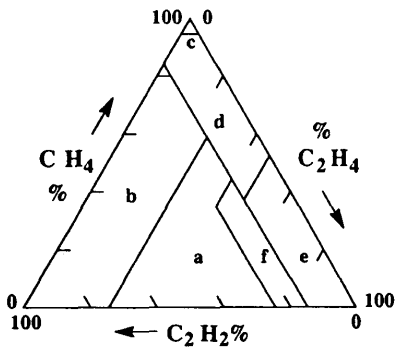
\includegraphics[width=0.5\textwidth]{BAB-2/figures/duval triangle.png}	
	    \caption{Segitiga Duval \cite{duval1989dissolved}}
	    \label{gambar:duval triangle}
	\end{center}
\end{figure}

\subsection{Kualitas Minyak Transformator}
Pada sebuah transformator daya peranan minyak adalah sebagai isolator cair, penghantar panas ke udara luar serta pelindung bagian dalam. Adapun fungsi sebagai isolator cair adalah untuk mencegah adanya loncatan listrik keluar karena pada umumnya transformator daya beroperasi pada tegangan tinggi. Kegunaan minyak transformator sebagai penghantar panas adalah untuk menjaga kestabilan suhu transformator karena adanya rugi-rugi daya yang berubah menjadi kalor. Sedangkan sebagai pelindung adalah untuk mencegah adanya reaksi kimia dari logam bagian dalam terhadap oksigen yang dapat menyebabkan adanya korosi \cite{pln2003panduan}.

Minyak transformator daya dapat beroperasi dengan baik jika belum melampaui batasan-batasan standar yang ditetapkan di antaranya tingkat keasaman serta kandungan airnya yang dapat diketahui melalui pengujian secara kimia \cite{ieee2007ieee}. Selain itu pengujian secara fisik dapat diperoleh \textit{interfacial tension} yang menjadi indikator banyaknya kontaminan polar tang terlarut dalam minyak \cite{sutaryono2015analisa}. Adapun pengujian elektrik dapat membantu mengetahui batas ambang tegangan yang dapat ditahan oleh bahan dielektrik transformator daya, hal ini dengan tegangan tembus (\textit{breakdown voltage}). Semakin tinggi nilai dari tegangan tembusnya maka semakin aman suatu transformator daya untuk dioperasikan. Tegangan tembus terjadi karena adanya elektron bebas pada bahan dielektrik, adanya elektron bebas pada bahan dielektrik disebabkan keberadaan kontaminan baik berupa gas, cair maupun padat pada sistem isolasi. Standar yang dijadikan rujukan untuk mengetahui kondisi minyak transformator adalah IEC 60422-2013 \cite{standard2013mineral}.

\begin{table}[h]
	\centering
	\caption{Standar Pengujian Minyak Tranformator}
	\label{tabel:standar minyak}
	\begin{tabular}{|c|c|c|c|c|c|} 
		\hline
		\multirow{2}{*}{\textbf{Parameter Uji}}                                                                 & \multirow{2}{*}{\textbf{Metode}}                   & \multicolumn{3}{c|}{\textbf{\textit{Score }(Si) batas IEC 60422:2013}} & \multirow{2}{*}{\begin{tabular}[c]{@{}c@{}}\textbf{Weight}\\~(Wi)\end{tabular}}  \\ 
		\cline{3-5}
		&                                                    & \textit{Good}(1) & \textit{Fair (2)} & Poor (3)                        &                                                                                  \\ 
		\hline
		\begin{tabular}[c]{@{}c@{}}\textbf{Tegangan Tembus}\\\textbf{(kV/2.5mm)}\end{tabular}                   & IEC 156                                            &  50              & 40 - 50           &  40                             & 3                                                                                \\ 
		\hline
		\begin{tabular}[c]{@{}c@{}}\textbf{Kandungan Air}\\\textbf{(mg/kg)}\end{tabular}                        & \begin{tabular}[c]{@{}c@{}}IEC\\60814\end{tabular} &  20              & 20 - 30           &  30                             & 4                                                                                \\ 
		\hline
		\begin{tabular}[c]{@{}c@{}}\textbf{Keasaman}\\\textbf{(mgKOH/g)}\end{tabular}                           & C2011K06                                           &  0.1             & 0.15 - 0.2        &  0.2                            & 1                                                                                \\ 
		\hline
		\begin{tabular}[c]{@{}c@{}}\textit{\textbf{Interfacial Tension}}\\\textit{\textbf{(mN/m)}}\end{tabular} & ISO 6295                                           &  28              & 22 - 28           &  22                             & 2                                                                                \\
		\hline
	\end{tabular}
\end{table}

\subsection{Pengujian Furan}
Seiring menurunnya umur dari minyak transformator daya akan membentuk suatu senyawa kimia yang dikenal dengan furan. Pembentukan furan juga disebabkan adanya suhu yang tinggi serta proses oksidasi senyawa asam. kerusakan akibat peningkatan konsentrasi di udara serta keberadaan oksigen dapat meningkatkan proses pembentukan furan. Keberadaan furan dapat menjadi acuan mengenai umur dari dielektrik padat yang berupa kertas. Standar pengujian furan disajikan pada Tabel \ref{tabel:standar furan} \cite{sutaryono2015analisa}.

\begin{table}[h]
	\centering
	\caption{Standar Pengujian Furan}
	\label{tabel:standar furan}
	\begin{tabular}{|c|c|c|c|} 
		\hline
		\textbf{No} & \begin{tabular}[c]{@{}c@{}}\textbf{2 FAL saat 55$^{\circ}$C }\\\textbf{(ppb)}\end{tabular} & \begin{tabular}[c]{@{}c@{}}\textbf{Estimasi }\\\textbf{~Umur Kertas (\%)}\end{tabular} & \textbf{Keterangan}                                          \\ 
		\hline
		1           & 58                                                                               & 100                                                                                    & \multirow{3}{*}{Penuaan Normal}                       \\ 
		\cline{1-3}
		2           & 130                                                                              & 90                                                                                     &                                                              \\ 
		\cline{1-3}
		3           & 292                                                                              & 79                                                                                     &                                                              \\ 
		\hline
		4           & 654                                                                              & 66                                                                                     & \multirow{4}{*}{Percepatan Penuaan}                   \\ 
		\cline{1-3}
		5           & 1464                                                                             & 50                                                                                     &                                                              \\ 
		\cline{1-3}
		6           & 1720                                                                             & 46                                                                                     &                                                              \\ 
		\cline{1-3}
		7           & 2021                                                                             & 42                                                                                     &                                                              \\ 
		\hline
		8           & 2374                                                                             & 38                                                                                     & \multirow{3}{*}{Daerah Peringatan : Penuaan Tidak Normal}  \\ 
		\cline{1-3}
		9           & 2789                                                                             & 33                                                                                     &                                                              \\ 
		\cline{1-3}
		10          & 3277                                                                             & 29                                                                                     &                                                              \\ 
		\hline
		11          & 3851                                                                             & 24                                                                                     & \multirow{2}{*}{Sangat Rentan Gangguan}             \\ 
		\cline{1-3}
		12          & 4524                                                                             & 19                                                                                     &                                                              \\ 
		\hline
		13          & 5315                                                                             & 13                                                                                     & \multirow{3}{*}{Akhir Pemakaian Kertas}                   \\ 
		\cline{1-3}
		14          & 6245                                                                             & 7                                                                                      &                                                              \\ 
		\cline{1-3}
		15          & 7337                                                                             & 0                                                                                      &                                                              \\
		\hline
	\end{tabular}
\end{table}



%Furan adalah senyawa organik yang terbentuk karena penurunan
%nilai minyak isolasi, panas berlebih, dan oksidasi asam. Kerusakan yang
%disebabkan oleh kelembaban ditambah dengan oksigen mempercepat
%penghancuran isolasi dan membentuk senyawa furan. Kandungan furan
%pada minyak sangat menentukan sisa usia dari kertas isolasi. Estimasi
%umur kertas isolasi berdasarkan jumlah konsentrasi furan yang ada di
%dalam minyak isolasi ditampilkan pada Tabel 2.3.




\section{\textit{Machine Learning}}
Machine learning merupakan salah satu metode yang digunakan dalam mempelajari pola serangkaian data dengan proses komputasi digital \cite{jordan2015machine}. Secara sederhana algoritma dirancang untuk digunakan dalam mempelajari suatu data kemudian dapat melakukan prediksi berdasarkan \textit{input} baru yang diberikan. Berdasarkan cara belajarnya terdapat pengelompokkan pada \textit{machine learning} yakni \textit{supervised learning} dan \textit{unsupervised learning} . Pada \textit{supervised learning} model dapat mempelajari data yang memiliki fitur yang dilengkapi dengan data target, sedangkan pada \textit{unsupervised learning} model belajar tanpa menggunakan adanya data target sehingga pada proses prediksi model akan memberikan keluaran berupa pengelompokan data \cite{alpaydin2020introduction}.

\textit{Machine Learning} telah mengalami banyak modifikasi untuk menyesuaikan jenis data yang diolah.  Arsitektur baru dari \textit{machine learning} yang banyak digunakan saat ini berupa algoritma yang meniru sistem kerja syaraf manusia yang dikenal dengan algoritma \textit{Artificial Neural Network} (ANN) \cite{braspenning1995artificial}. Dengan menggunakan ANN sistem memungkinkan dalam mengenali objek dalam sebuah gambar merupakan salah satu implementasinya. Adapun pada pengolahan data yang bersifat \textit{time series} atau berupa deret ANN dikembangkan agar dapat melakukan sebuah prediksi berdasarkan \textit{input} yang diterima sebelumnya sebagai dasar referensi prediksi ke depan. Model tersebut dikenal dengan \textit{Recurrent Neural Network} dimana setiap \textit{input} yang diterima sebelum dilakukan prediksi akan diproses secara berulang pada satu sel RNN sehingga model dapat mengingat informasi pentingnya \cite{medsker2001recurrent}.


\section{\textit{Long Short Term Memory (LSTM)}}
Pada pemodelan dengan menggunakan metode RNN secara umum memiliki kemampuan dalam membuat prediksi yang dipengaruhi oleh \textit{input} sebelumnya. Namun, terdapat kekurangan pada metode tersebut yakni tidak mampu mengatasi dengan  seri yang panjang, misalnya pada sebuah data \textit{time series}, RNN akan sulit mengkorelasikan antara data saat ini dengan data yang sangat lampau, akibatnya jika data yang diproses dalam rentang waktu yang lama maka RNN hanya mampu membuat prediksi yang hanya berkaitan pada waktu yang pendek. Kekurangan pada RNN dikarenakan adanya \textit{vanising gradient}, yakni menghapus data yang tidak berkaitan dengan data baru yang dimasukkan. Adanya kekurangan tersebut maka dibutuhkan suatu metode baru yang dapat mengingat data lampau saat menerima \textit{input} terbaru. LSTM merupakan salah satu turunan dari pemodelan matematis yang digunakan dalam mengenali pola serangkaian data. Sel LSTM dalam sebuah jaringan dapat dilihat pada \ref{gambar:sel LSTM}.
\begin{figure}[h]
	\begin{center}
		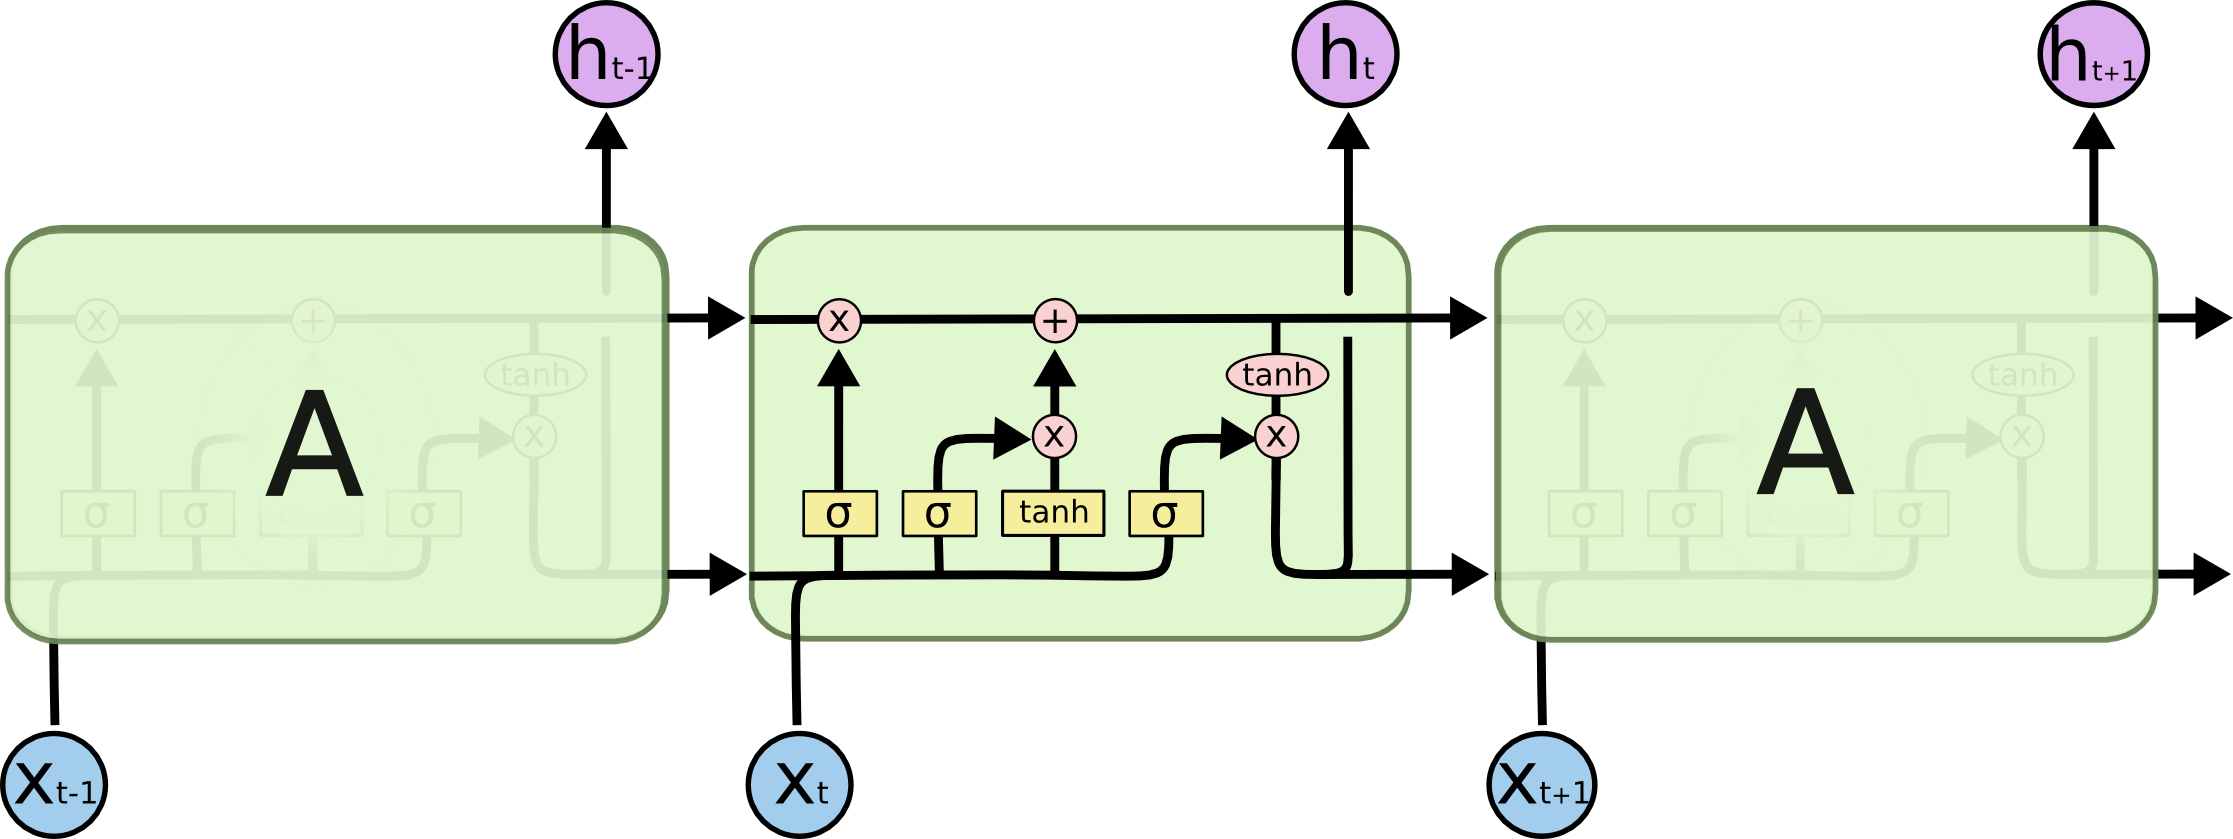
\includegraphics[width=0.7\textwidth]{BAB-2/figures/LSTM3-chain.png}	
		\caption{Sel LSTM \cite{olah2015understanding}}
		\label{gambar:sel LSTM}
	\end{center}
\end{figure}

Kelebihan yang dimiliki LSTM dibandingkan dengan RNN dikarenakan algoritma yang digunakan terdiri dari struktur yang kompleks. Secara umum terdapat 4 bagian pada arsitektur LSTM yakni \textit{forget gate}, \textit{input gate}, \textit{Cell gate}, dan \textit{Output gate}. 
\subsection{\textit{Forget Gate}}
%\begin{figure}[h]
%	\begin{center}
%		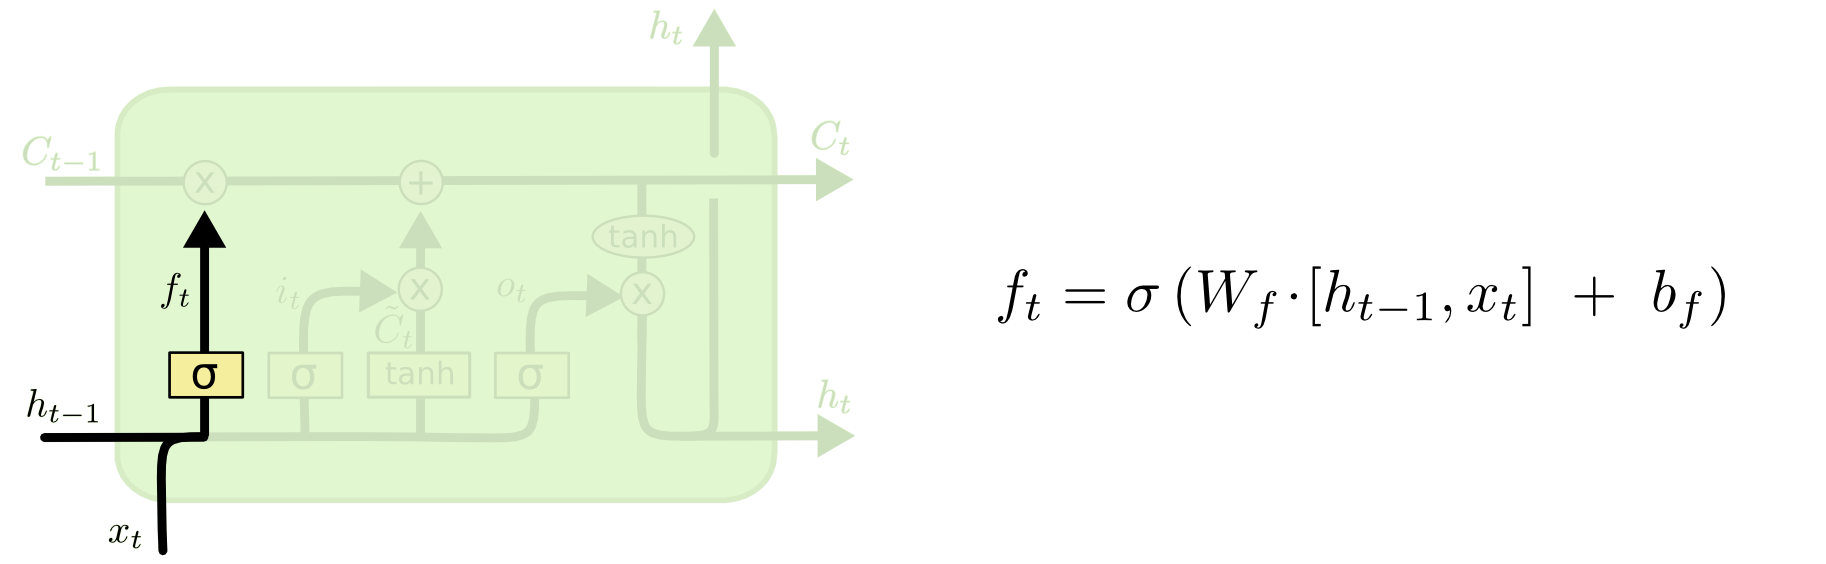
\includegraphics[width=0.7\textwidth]{BAB-2/figures/LSTM3-focus-f.png}	
%		\caption{Forget Gate \cite{olah2015understanding}}
%		\label{gambar:forget gate}
%	\end{center}
%\end{figure}


Pada \textit{Forget gate} merupakan bagian yang menentukan mengenai informasi pada keluaran sel sebelumnya untuk dipertahankan atau dihapus. Hal ini dilakukan dengan memasukkan keluaran sel sebelumnya yang digabungkan dengan masukan baru ke dalam fungsi aktivasi \textit{sigmoid}. Informasi akan dipertahankan untuk hasil dari \textit{sigmoid} dengan nilai 1 dan dihapus untuk keluaran yang bernilai 0. Secara matematis pada \textit{forget gate} digunakan persamaan sebagai berikut:
\begin{equation}
	\boldsymbol{f_t} = \sigma_g(\boldsymbol{W_{f}}.[\boldsymbol{h_{t-1}}, \boldsymbol{x_t}] + \boldsymbol{b_f})
	\label{func:forget}
\end{equation} 

\centerline{
	\begin{minipage}{\linewidth}
		\vspace{12 pt}
		\centering
		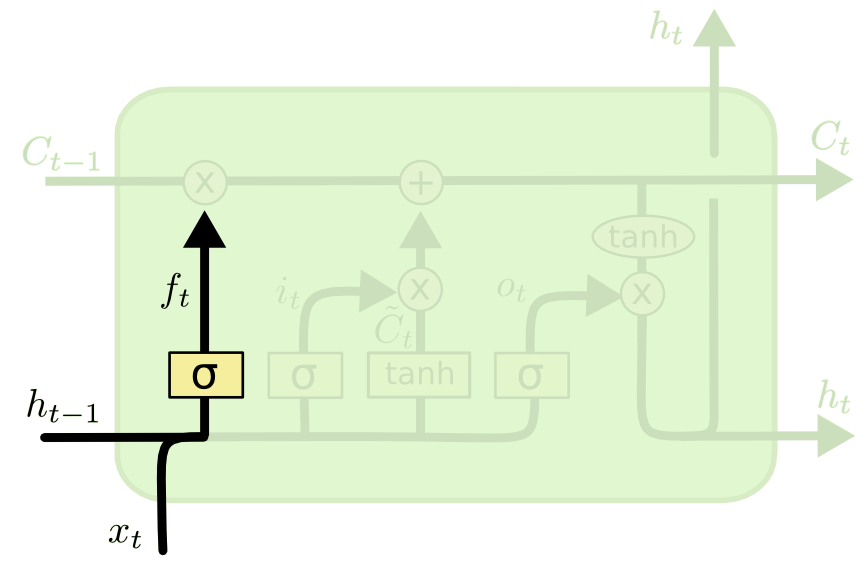
\includegraphics[width=0.4\textwidth]{BAB-2/figures/LSTM-forget.png}	
		\captionof{figure}{Forget Gate \cite{olah2015understanding}}
		\label{gambar:forget gate}
	\end{minipage}
}

Berdasarkan persamaan~(\ref{func:forget}) dapat diketahui pada persamaan tersebut terdapat bentuk $[\boldsymbol{h_{t-1}}, \boldsymbol{x_t}]$. Hal ini merupakan operasi penggabungan vektor yakni penggabungan baris pada $\boldsymbol{h_{t-1}}$ dengan baris pada $\boldsymbol{x_t}$.
\subsection{\textit{Input Gate}}
Salah satu kelebihan LSTM adalah dapat mengingat informasi data masukan yang lama. Hal ini dikarenakan karena adanya satu bagian yang berperan dalam memperbarui memori berdasarkan informasi penting dari masukan baru. Kemampuan ini diperoleh karena ada dua tahapan penting pada \textit{input gate} yakni melalui lapisan \textit{sigmoid} dan \textit{tanh}. lapisan akan memberikan keluaran berupa nilai mana saja yang harus dilakukan pembaruan pada memori sedangkan lapisan \textit{tanh} memberikan keluaran berupa calon ($\boldsymbol{\tilde{C}}$) yang ditambahkan pada memori. 
\begin{equation}
	\boldsymbol{i_t} = \sigma_i(\boldsymbol{W_{f}}.[\boldsymbol{h_{t-1}}, \boldsymbol{x_t}] + \boldsymbol{b_i})\\
	\label{func:input}
\end{equation}
\begin{equation}
	\boldsymbol{\tilde{C}} = tanh(\boldsymbol{W_{C}}.[\boldsymbol{h_{t-1}}, \boldsymbol{x_t}] + \boldsymbol{b_C})
	\label{func:C-tilde}
\end{equation}

\centerline{
	\begin{minipage}{\linewidth}
		\vspace{12 pt}
		\centering
		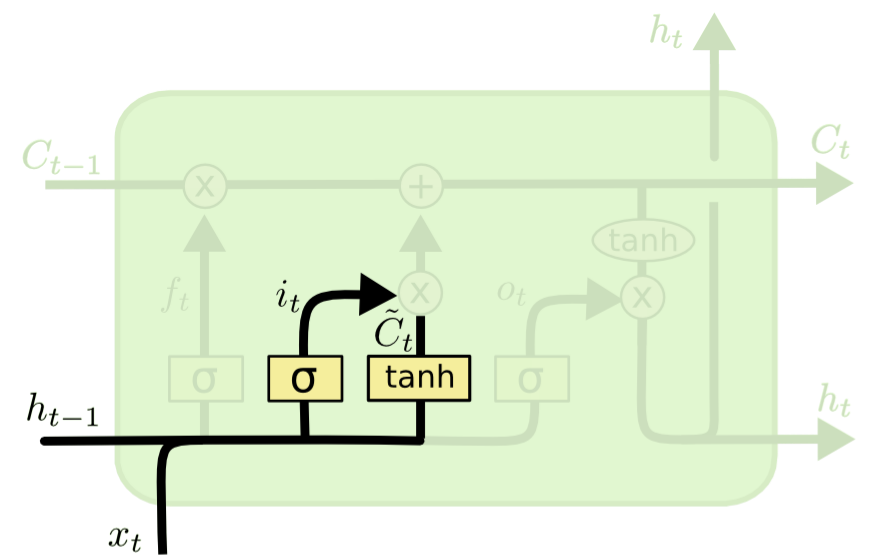
\includegraphics[width=0.4\textwidth]{BAB-2/figures/LSTM-input.png}	
		\captionof{figure}{Input Gate \cite{olah2015understanding}}
		\label{gambar:input gate}
	\end{minipage}
}

Hasil perkalian dari dua lapisan pada \textit{input gate} akan menjadi \textit{input} pada memori sebagai pembaruan. pembaruan yang terjadi dalam hanya dalam jumlah yang sedikit, oleh karena itu informasi penting pada data yang lampau akan tetap tersimpan untuk jumlah data yang banyak.
\subsection{\textit{Cell gate}}
\textit{Cell gate} merupakan tempat penyimpanan informasi penting pada setiap data yang diberikan pada LSTM. \textit{cell gate} terdiri dari masukan dari \textit{forget gate} untuk mengurangi informasi yang tidak diperlukan dari semua masukan sebelumnya melalui persamaan ~(\ref{func:forget}). Kemudian ditambahkan dengan hasil perkalian dari $\boldsymbol{i_t}$ dan $\boldsymbol{\tilde{C}}$.
\begin{equation}
	\boldsymbol{C_t} = \boldsymbol{f_t}*\boldsymbol{C_{t-1}} + \boldsymbol{i_t} * \boldsymbol{\tilde{C}}
	\label{func:cell_gate}
\end{equation}

\centerline{
	\begin{minipage}{\linewidth}
		\vspace{12 pt}
		\centering
		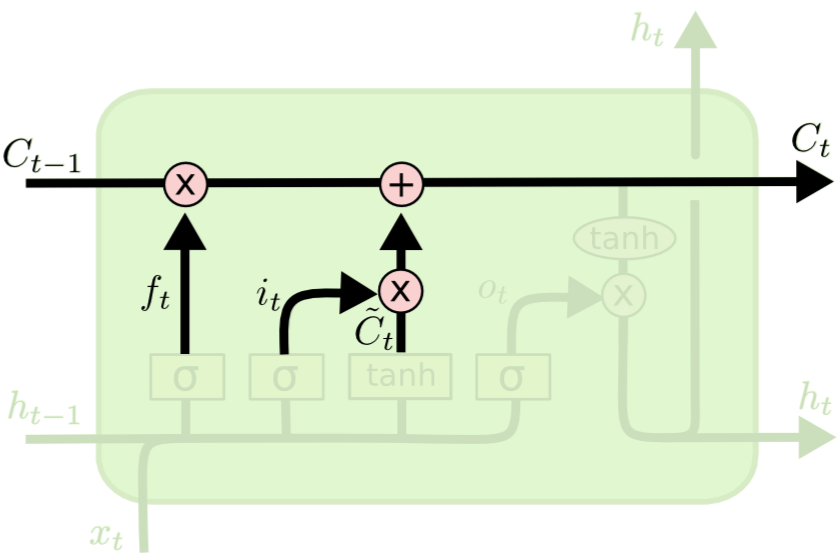
\includegraphics[width=0.4\textwidth]{BAB-2/figures/LSTM-cell.png}	
		\captionof{figure}{Cell Gate \cite{olah2015understanding}}
		\label{gambar:cell gate}
	\end{minipage}
}
Hal utama yang perlu diperhatikan adalah bahwa pada LSTM bagian \textit{cell gate} merupakan lapisan yang saling terhubung, sehingga antar sel yang berjauhan pun dapat terintegrasi. Kondisi ini yang menjadikan LSTM dapat mengatasi permasalahan versi RNN sebelumnya yang diakibatkan adanya \textit{vanishing gradient}.
\subsection{\textit{Output Gate}}
Pada bagian akhir merupakan keluaran dari sel LSTM atau dapat berupa hasil prediksi berdasarkan masukan yang diberikan. Keluaran ditentukan oleh memori $\boldsymbol{C_t}$ dan masukan yang diberikan. Hal ini dilakukan dengan memasukkan  $\boldsymbol{x_t}$ dan keluaran sebelumnya ($\boldsymbol{h_{t-1}}$) pada fungsi \textit{sigmoid}. Hasil dari fungsi \textit{sigmoid} kemudian akan memfilter nilai dari \textit{cell state} yang dapat diteruskan menuju keluaran. Sebelum dikalikan dengan hasil dari gerbang \textit{sigmoid}, \textit{cell state} terlebih dahulu melewati gerbang tanh untuk mengubah nilai pada rentang -1 sampai 1. Secara matematis dapat dituliskan sebagai berikut:
\begin{equation}
	\boldsymbol{o_t} = \sigma(\boldsymbol{W_i}.[\boldsymbol{h_{t-1}}, \boldsymbol{x_t}] + \boldsymbol{b_o})
	\label{func:ouput_sigmoid}
\end{equation}
\begin{equation}
	\boldsymbol{h_t} = \boldsymbol{o_t}*tanh(\boldsymbol{C_t})
	\label{func:final_output}
\end{equation}
\centerline{
	\begin{minipage}{\linewidth}
		\vspace{12 pt}
		\centering
		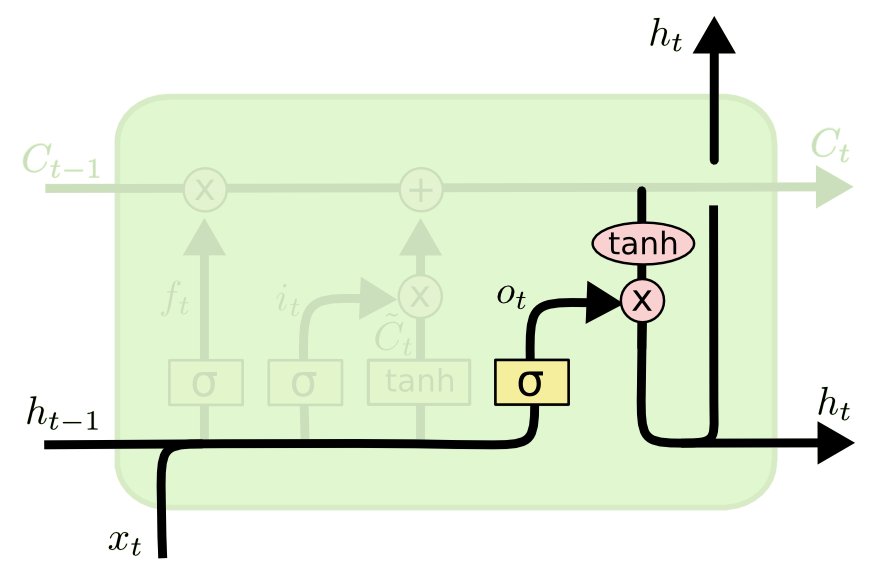
\includegraphics[width=0.4\textwidth]{BAB-2/figures/LSTM-output.png}	
		\captionof{figure}{Output Gate \cite{olah2015understanding}}
		\label{gambar:output gate}
	\end{minipage}
}

\section{Fungsi Aktivasi}
Fungsi aktivasi merupakan sebuah fungsi matematis yang diterapkan setiap keluaran dari \textit{neuron} pada pemodelan ANN. Model LSTM pada dasarnya dibentuk berdasarkan model dari ANN, sehingga arsitekturnya menggunakan fungsi aktivasi. Hampir di setiap bagian pada LSTM terdapat adanya fungsi aktivasi. Pada model LSTM, umumnya melibatkan dua fungsi aktivasi yakni \textit{tanh} dan \textit{sigmoid}($\sigma$). Selain fungsi aktivasi tersebut terdapat juga jenis yang lain. Secara detail persamaan fungsi aktivasi dan plot grafik adalah sebagai berikut:

\textit{Sigmoid}:
\begin{equation}
	\sigma (x) = \frac{1}{1 + e^{-x}}
	\label{func:sigmoid}
\end{equation}

\centerline{
	\begin{minipage}{\linewidth}
		\vspace{12 pt}
		\centering
		%% Creator: Matplotlib, PGF backend
%%
%% To include the figure in your LaTeX document, write
%%   \input{<filename>.pgf}
%%
%% Make sure the required packages are loaded in your preamble
%%   \usepackage{pgf}
%%
%% Figures using additional raster images can only be included by \input if
%% they are in the same directory as the main LaTeX file. For loading figures
%% from other directories you can use the `import` package
%%   \usepackage{import}
%%
%% and then include the figures with
%%   \import{<path to file>}{<filename>.pgf}
%%
%% Matplotlib used the following preamble
%%   \usepackage{fontspec}
%%   \setmainfont{DejaVuSerif.ttf}[Path=\detokenize{/home/alfa/.local/lib/python3.8/site-packages/matplotlib/mpl-data/fonts/ttf/}]
%%   \setsansfont{DejaVuSans.ttf}[Path=\detokenize{/home/alfa/.local/lib/python3.8/site-packages/matplotlib/mpl-data/fonts/ttf/}]
%%   \setmonofont{DejaVuSansMono.ttf}[Path=\detokenize{/home/alfa/.local/lib/python3.8/site-packages/matplotlib/mpl-data/fonts/ttf/}]
%%
\begingroup%
\makeatletter%
\begin{pgfpicture}%
\pgfpathrectangle{\pgfpointorigin}{\pgfqpoint{3.805602in}{2.119135in}}%
\pgfusepath{use as bounding box, clip}%
\begin{pgfscope}%
\pgfsetbuttcap%
\pgfsetmiterjoin%
\pgfsetlinewidth{0.000000pt}%
\definecolor{currentstroke}{rgb}{1.000000,1.000000,1.000000}%
\pgfsetstrokecolor{currentstroke}%
\pgfsetstrokeopacity{0.000000}%
\pgfsetdash{}{0pt}%
\pgfpathmoveto{\pgfqpoint{0.000000in}{0.000000in}}%
\pgfpathlineto{\pgfqpoint{3.805602in}{0.000000in}}%
\pgfpathlineto{\pgfqpoint{3.805602in}{2.119135in}}%
\pgfpathlineto{\pgfqpoint{0.000000in}{2.119135in}}%
\pgfpathclose%
\pgfusepath{}%
\end{pgfscope}%
\begin{pgfscope}%
\pgfsetbuttcap%
\pgfsetmiterjoin%
\definecolor{currentfill}{rgb}{1.000000,1.000000,1.000000}%
\pgfsetfillcolor{currentfill}%
\pgfsetlinewidth{0.000000pt}%
\definecolor{currentstroke}{rgb}{0.000000,0.000000,0.000000}%
\pgfsetstrokecolor{currentstroke}%
\pgfsetstrokeopacity{0.000000}%
\pgfsetdash{}{0pt}%
\pgfpathmoveto{\pgfqpoint{0.318102in}{0.231635in}}%
\pgfpathlineto{\pgfqpoint{3.805602in}{0.231635in}}%
\pgfpathlineto{\pgfqpoint{3.805602in}{2.119135in}}%
\pgfpathlineto{\pgfqpoint{0.318102in}{2.119135in}}%
\pgfpathclose%
\pgfusepath{fill}%
\end{pgfscope}%
\begin{pgfscope}%
\pgfpathrectangle{\pgfqpoint{0.318102in}{0.231635in}}{\pgfqpoint{3.487500in}{1.887500in}}%
\pgfusepath{clip}%
\pgfsetrectcap%
\pgfsetroundjoin%
\pgfsetlinewidth{0.803000pt}%
\definecolor{currentstroke}{rgb}{0.890196,0.882353,0.882353}%
\pgfsetstrokecolor{currentstroke}%
\pgfsetdash{}{0pt}%
\pgfpathmoveto{\pgfqpoint{0.476624in}{0.231635in}}%
\pgfpathlineto{\pgfqpoint{0.476624in}{2.119135in}}%
\pgfusepath{stroke}%
\end{pgfscope}%
\begin{pgfscope}%
\pgfsetbuttcap%
\pgfsetroundjoin%
\definecolor{currentfill}{rgb}{0.000000,0.000000,0.000000}%
\pgfsetfillcolor{currentfill}%
\pgfsetlinewidth{0.803000pt}%
\definecolor{currentstroke}{rgb}{0.000000,0.000000,0.000000}%
\pgfsetstrokecolor{currentstroke}%
\pgfsetdash{}{0pt}%
\pgfsys@defobject{currentmarker}{\pgfqpoint{0.000000in}{-0.048611in}}{\pgfqpoint{0.000000in}{0.000000in}}{%
\pgfpathmoveto{\pgfqpoint{0.000000in}{0.000000in}}%
\pgfpathlineto{\pgfqpoint{0.000000in}{-0.048611in}}%
\pgfusepath{stroke,fill}%
}%
\begin{pgfscope}%
\pgfsys@transformshift{0.476624in}{0.231635in}%
\pgfsys@useobject{currentmarker}{}%
\end{pgfscope}%
\end{pgfscope}%
\begin{pgfscope}%
\definecolor{textcolor}{rgb}{0.000000,0.000000,0.000000}%
\pgfsetstrokecolor{textcolor}%
\pgfsetfillcolor{textcolor}%
\pgftext[x=0.476624in,y=0.134413in,,top]{\color{textcolor}\sffamily\fontsize{10.000000}{12.000000}\selectfont \ensuremath{-}6}%
\end{pgfscope}%
\begin{pgfscope}%
\pgfpathrectangle{\pgfqpoint{0.318102in}{0.231635in}}{\pgfqpoint{3.487500in}{1.887500in}}%
\pgfusepath{clip}%
\pgfsetrectcap%
\pgfsetroundjoin%
\pgfsetlinewidth{0.803000pt}%
\definecolor{currentstroke}{rgb}{0.890196,0.882353,0.882353}%
\pgfsetstrokecolor{currentstroke}%
\pgfsetdash{}{0pt}%
\pgfpathmoveto{\pgfqpoint{1.009474in}{0.231635in}}%
\pgfpathlineto{\pgfqpoint{1.009474in}{2.119135in}}%
\pgfusepath{stroke}%
\end{pgfscope}%
\begin{pgfscope}%
\pgfsetbuttcap%
\pgfsetroundjoin%
\definecolor{currentfill}{rgb}{0.000000,0.000000,0.000000}%
\pgfsetfillcolor{currentfill}%
\pgfsetlinewidth{0.803000pt}%
\definecolor{currentstroke}{rgb}{0.000000,0.000000,0.000000}%
\pgfsetstrokecolor{currentstroke}%
\pgfsetdash{}{0pt}%
\pgfsys@defobject{currentmarker}{\pgfqpoint{0.000000in}{-0.048611in}}{\pgfqpoint{0.000000in}{0.000000in}}{%
\pgfpathmoveto{\pgfqpoint{0.000000in}{0.000000in}}%
\pgfpathlineto{\pgfqpoint{0.000000in}{-0.048611in}}%
\pgfusepath{stroke,fill}%
}%
\begin{pgfscope}%
\pgfsys@transformshift{1.009474in}{0.231635in}%
\pgfsys@useobject{currentmarker}{}%
\end{pgfscope}%
\end{pgfscope}%
\begin{pgfscope}%
\definecolor{textcolor}{rgb}{0.000000,0.000000,0.000000}%
\pgfsetstrokecolor{textcolor}%
\pgfsetfillcolor{textcolor}%
\pgftext[x=1.009474in,y=0.134413in,,top]{\color{textcolor}\sffamily\fontsize{10.000000}{12.000000}\selectfont \ensuremath{-}4}%
\end{pgfscope}%
\begin{pgfscope}%
\pgfpathrectangle{\pgfqpoint{0.318102in}{0.231635in}}{\pgfqpoint{3.487500in}{1.887500in}}%
\pgfusepath{clip}%
\pgfsetrectcap%
\pgfsetroundjoin%
\pgfsetlinewidth{0.803000pt}%
\definecolor{currentstroke}{rgb}{0.890196,0.882353,0.882353}%
\pgfsetstrokecolor{currentstroke}%
\pgfsetdash{}{0pt}%
\pgfpathmoveto{\pgfqpoint{1.542323in}{0.231635in}}%
\pgfpathlineto{\pgfqpoint{1.542323in}{2.119135in}}%
\pgfusepath{stroke}%
\end{pgfscope}%
\begin{pgfscope}%
\pgfsetbuttcap%
\pgfsetroundjoin%
\definecolor{currentfill}{rgb}{0.000000,0.000000,0.000000}%
\pgfsetfillcolor{currentfill}%
\pgfsetlinewidth{0.803000pt}%
\definecolor{currentstroke}{rgb}{0.000000,0.000000,0.000000}%
\pgfsetstrokecolor{currentstroke}%
\pgfsetdash{}{0pt}%
\pgfsys@defobject{currentmarker}{\pgfqpoint{0.000000in}{-0.048611in}}{\pgfqpoint{0.000000in}{0.000000in}}{%
\pgfpathmoveto{\pgfqpoint{0.000000in}{0.000000in}}%
\pgfpathlineto{\pgfqpoint{0.000000in}{-0.048611in}}%
\pgfusepath{stroke,fill}%
}%
\begin{pgfscope}%
\pgfsys@transformshift{1.542323in}{0.231635in}%
\pgfsys@useobject{currentmarker}{}%
\end{pgfscope}%
\end{pgfscope}%
\begin{pgfscope}%
\definecolor{textcolor}{rgb}{0.000000,0.000000,0.000000}%
\pgfsetstrokecolor{textcolor}%
\pgfsetfillcolor{textcolor}%
\pgftext[x=1.542323in,y=0.134413in,,top]{\color{textcolor}\sffamily\fontsize{10.000000}{12.000000}\selectfont \ensuremath{-}2}%
\end{pgfscope}%
\begin{pgfscope}%
\pgfpathrectangle{\pgfqpoint{0.318102in}{0.231635in}}{\pgfqpoint{3.487500in}{1.887500in}}%
\pgfusepath{clip}%
\pgfsetrectcap%
\pgfsetroundjoin%
\pgfsetlinewidth{0.803000pt}%
\definecolor{currentstroke}{rgb}{0.890196,0.882353,0.882353}%
\pgfsetstrokecolor{currentstroke}%
\pgfsetdash{}{0pt}%
\pgfpathmoveto{\pgfqpoint{2.075173in}{0.231635in}}%
\pgfpathlineto{\pgfqpoint{2.075173in}{2.119135in}}%
\pgfusepath{stroke}%
\end{pgfscope}%
\begin{pgfscope}%
\pgfsetbuttcap%
\pgfsetroundjoin%
\definecolor{currentfill}{rgb}{0.000000,0.000000,0.000000}%
\pgfsetfillcolor{currentfill}%
\pgfsetlinewidth{0.803000pt}%
\definecolor{currentstroke}{rgb}{0.000000,0.000000,0.000000}%
\pgfsetstrokecolor{currentstroke}%
\pgfsetdash{}{0pt}%
\pgfsys@defobject{currentmarker}{\pgfqpoint{0.000000in}{-0.048611in}}{\pgfqpoint{0.000000in}{0.000000in}}{%
\pgfpathmoveto{\pgfqpoint{0.000000in}{0.000000in}}%
\pgfpathlineto{\pgfqpoint{0.000000in}{-0.048611in}}%
\pgfusepath{stroke,fill}%
}%
\begin{pgfscope}%
\pgfsys@transformshift{2.075173in}{0.231635in}%
\pgfsys@useobject{currentmarker}{}%
\end{pgfscope}%
\end{pgfscope}%
\begin{pgfscope}%
\definecolor{textcolor}{rgb}{0.000000,0.000000,0.000000}%
\pgfsetstrokecolor{textcolor}%
\pgfsetfillcolor{textcolor}%
\pgftext[x=2.075173in,y=0.134413in,,top]{\color{textcolor}\sffamily\fontsize{10.000000}{12.000000}\selectfont 0}%
\end{pgfscope}%
\begin{pgfscope}%
\pgfpathrectangle{\pgfqpoint{0.318102in}{0.231635in}}{\pgfqpoint{3.487500in}{1.887500in}}%
\pgfusepath{clip}%
\pgfsetrectcap%
\pgfsetroundjoin%
\pgfsetlinewidth{0.803000pt}%
\definecolor{currentstroke}{rgb}{0.890196,0.882353,0.882353}%
\pgfsetstrokecolor{currentstroke}%
\pgfsetdash{}{0pt}%
\pgfpathmoveto{\pgfqpoint{2.608022in}{0.231635in}}%
\pgfpathlineto{\pgfqpoint{2.608022in}{2.119135in}}%
\pgfusepath{stroke}%
\end{pgfscope}%
\begin{pgfscope}%
\pgfsetbuttcap%
\pgfsetroundjoin%
\definecolor{currentfill}{rgb}{0.000000,0.000000,0.000000}%
\pgfsetfillcolor{currentfill}%
\pgfsetlinewidth{0.803000pt}%
\definecolor{currentstroke}{rgb}{0.000000,0.000000,0.000000}%
\pgfsetstrokecolor{currentstroke}%
\pgfsetdash{}{0pt}%
\pgfsys@defobject{currentmarker}{\pgfqpoint{0.000000in}{-0.048611in}}{\pgfqpoint{0.000000in}{0.000000in}}{%
\pgfpathmoveto{\pgfqpoint{0.000000in}{0.000000in}}%
\pgfpathlineto{\pgfqpoint{0.000000in}{-0.048611in}}%
\pgfusepath{stroke,fill}%
}%
\begin{pgfscope}%
\pgfsys@transformshift{2.608022in}{0.231635in}%
\pgfsys@useobject{currentmarker}{}%
\end{pgfscope}%
\end{pgfscope}%
\begin{pgfscope}%
\definecolor{textcolor}{rgb}{0.000000,0.000000,0.000000}%
\pgfsetstrokecolor{textcolor}%
\pgfsetfillcolor{textcolor}%
\pgftext[x=2.608022in,y=0.134413in,,top]{\color{textcolor}\sffamily\fontsize{10.000000}{12.000000}\selectfont 2}%
\end{pgfscope}%
\begin{pgfscope}%
\pgfpathrectangle{\pgfqpoint{0.318102in}{0.231635in}}{\pgfqpoint{3.487500in}{1.887500in}}%
\pgfusepath{clip}%
\pgfsetrectcap%
\pgfsetroundjoin%
\pgfsetlinewidth{0.803000pt}%
\definecolor{currentstroke}{rgb}{0.890196,0.882353,0.882353}%
\pgfsetstrokecolor{currentstroke}%
\pgfsetdash{}{0pt}%
\pgfpathmoveto{\pgfqpoint{3.140872in}{0.231635in}}%
\pgfpathlineto{\pgfqpoint{3.140872in}{2.119135in}}%
\pgfusepath{stroke}%
\end{pgfscope}%
\begin{pgfscope}%
\pgfsetbuttcap%
\pgfsetroundjoin%
\definecolor{currentfill}{rgb}{0.000000,0.000000,0.000000}%
\pgfsetfillcolor{currentfill}%
\pgfsetlinewidth{0.803000pt}%
\definecolor{currentstroke}{rgb}{0.000000,0.000000,0.000000}%
\pgfsetstrokecolor{currentstroke}%
\pgfsetdash{}{0pt}%
\pgfsys@defobject{currentmarker}{\pgfqpoint{0.000000in}{-0.048611in}}{\pgfqpoint{0.000000in}{0.000000in}}{%
\pgfpathmoveto{\pgfqpoint{0.000000in}{0.000000in}}%
\pgfpathlineto{\pgfqpoint{0.000000in}{-0.048611in}}%
\pgfusepath{stroke,fill}%
}%
\begin{pgfscope}%
\pgfsys@transformshift{3.140872in}{0.231635in}%
\pgfsys@useobject{currentmarker}{}%
\end{pgfscope}%
\end{pgfscope}%
\begin{pgfscope}%
\definecolor{textcolor}{rgb}{0.000000,0.000000,0.000000}%
\pgfsetstrokecolor{textcolor}%
\pgfsetfillcolor{textcolor}%
\pgftext[x=3.140872in,y=0.134413in,,top]{\color{textcolor}\sffamily\fontsize{10.000000}{12.000000}\selectfont 4}%
\end{pgfscope}%
\begin{pgfscope}%
\pgfpathrectangle{\pgfqpoint{0.318102in}{0.231635in}}{\pgfqpoint{3.487500in}{1.887500in}}%
\pgfusepath{clip}%
\pgfsetrectcap%
\pgfsetroundjoin%
\pgfsetlinewidth{0.803000pt}%
\definecolor{currentstroke}{rgb}{0.890196,0.882353,0.882353}%
\pgfsetstrokecolor{currentstroke}%
\pgfsetdash{}{0pt}%
\pgfpathmoveto{\pgfqpoint{3.673721in}{0.231635in}}%
\pgfpathlineto{\pgfqpoint{3.673721in}{2.119135in}}%
\pgfusepath{stroke}%
\end{pgfscope}%
\begin{pgfscope}%
\pgfsetbuttcap%
\pgfsetroundjoin%
\definecolor{currentfill}{rgb}{0.000000,0.000000,0.000000}%
\pgfsetfillcolor{currentfill}%
\pgfsetlinewidth{0.803000pt}%
\definecolor{currentstroke}{rgb}{0.000000,0.000000,0.000000}%
\pgfsetstrokecolor{currentstroke}%
\pgfsetdash{}{0pt}%
\pgfsys@defobject{currentmarker}{\pgfqpoint{0.000000in}{-0.048611in}}{\pgfqpoint{0.000000in}{0.000000in}}{%
\pgfpathmoveto{\pgfqpoint{0.000000in}{0.000000in}}%
\pgfpathlineto{\pgfqpoint{0.000000in}{-0.048611in}}%
\pgfusepath{stroke,fill}%
}%
\begin{pgfscope}%
\pgfsys@transformshift{3.673721in}{0.231635in}%
\pgfsys@useobject{currentmarker}{}%
\end{pgfscope}%
\end{pgfscope}%
\begin{pgfscope}%
\definecolor{textcolor}{rgb}{0.000000,0.000000,0.000000}%
\pgfsetstrokecolor{textcolor}%
\pgfsetfillcolor{textcolor}%
\pgftext[x=3.673721in,y=0.134413in,,top]{\color{textcolor}\sffamily\fontsize{10.000000}{12.000000}\selectfont 6}%
\end{pgfscope}%
\begin{pgfscope}%
\pgfpathrectangle{\pgfqpoint{0.318102in}{0.231635in}}{\pgfqpoint{3.487500in}{1.887500in}}%
\pgfusepath{clip}%
\pgfsetrectcap%
\pgfsetroundjoin%
\pgfsetlinewidth{0.803000pt}%
\definecolor{currentstroke}{rgb}{0.890196,0.882353,0.882353}%
\pgfsetstrokecolor{currentstroke}%
\pgfsetdash{}{0pt}%
\pgfpathmoveto{\pgfqpoint{0.318102in}{0.313165in}}%
\pgfpathlineto{\pgfqpoint{3.805602in}{0.313165in}}%
\pgfusepath{stroke}%
\end{pgfscope}%
\begin{pgfscope}%
\pgfsetbuttcap%
\pgfsetroundjoin%
\definecolor{currentfill}{rgb}{0.000000,0.000000,0.000000}%
\pgfsetfillcolor{currentfill}%
\pgfsetlinewidth{0.803000pt}%
\definecolor{currentstroke}{rgb}{0.000000,0.000000,0.000000}%
\pgfsetstrokecolor{currentstroke}%
\pgfsetdash{}{0pt}%
\pgfsys@defobject{currentmarker}{\pgfqpoint{-0.048611in}{0.000000in}}{\pgfqpoint{-0.000000in}{0.000000in}}{%
\pgfpathmoveto{\pgfqpoint{-0.000000in}{0.000000in}}%
\pgfpathlineto{\pgfqpoint{-0.048611in}{0.000000in}}%
\pgfusepath{stroke,fill}%
}%
\begin{pgfscope}%
\pgfsys@transformshift{0.318102in}{0.313165in}%
\pgfsys@useobject{currentmarker}{}%
\end{pgfscope}%
\end{pgfscope}%
\begin{pgfscope}%
\definecolor{textcolor}{rgb}{0.000000,0.000000,0.000000}%
\pgfsetstrokecolor{textcolor}%
\pgfsetfillcolor{textcolor}%
\pgftext[x=0.000000in, y=0.260404in, left, base]{\color{textcolor}\sffamily\fontsize{10.000000}{12.000000}\selectfont 0.0}%
\end{pgfscope}%
\begin{pgfscope}%
\pgfpathrectangle{\pgfqpoint{0.318102in}{0.231635in}}{\pgfqpoint{3.487500in}{1.887500in}}%
\pgfusepath{clip}%
\pgfsetrectcap%
\pgfsetroundjoin%
\pgfsetlinewidth{0.803000pt}%
\definecolor{currentstroke}{rgb}{0.890196,0.882353,0.882353}%
\pgfsetstrokecolor{currentstroke}%
\pgfsetdash{}{0pt}%
\pgfpathmoveto{\pgfqpoint{0.318102in}{0.658143in}}%
\pgfpathlineto{\pgfqpoint{3.805602in}{0.658143in}}%
\pgfusepath{stroke}%
\end{pgfscope}%
\begin{pgfscope}%
\pgfsetbuttcap%
\pgfsetroundjoin%
\definecolor{currentfill}{rgb}{0.000000,0.000000,0.000000}%
\pgfsetfillcolor{currentfill}%
\pgfsetlinewidth{0.803000pt}%
\definecolor{currentstroke}{rgb}{0.000000,0.000000,0.000000}%
\pgfsetstrokecolor{currentstroke}%
\pgfsetdash{}{0pt}%
\pgfsys@defobject{currentmarker}{\pgfqpoint{-0.048611in}{0.000000in}}{\pgfqpoint{-0.000000in}{0.000000in}}{%
\pgfpathmoveto{\pgfqpoint{-0.000000in}{0.000000in}}%
\pgfpathlineto{\pgfqpoint{-0.048611in}{0.000000in}}%
\pgfusepath{stroke,fill}%
}%
\begin{pgfscope}%
\pgfsys@transformshift{0.318102in}{0.658143in}%
\pgfsys@useobject{currentmarker}{}%
\end{pgfscope}%
\end{pgfscope}%
\begin{pgfscope}%
\definecolor{textcolor}{rgb}{0.000000,0.000000,0.000000}%
\pgfsetstrokecolor{textcolor}%
\pgfsetfillcolor{textcolor}%
\pgftext[x=0.000000in, y=0.605381in, left, base]{\color{textcolor}\sffamily\fontsize{10.000000}{12.000000}\selectfont 0.2}%
\end{pgfscope}%
\begin{pgfscope}%
\pgfpathrectangle{\pgfqpoint{0.318102in}{0.231635in}}{\pgfqpoint{3.487500in}{1.887500in}}%
\pgfusepath{clip}%
\pgfsetrectcap%
\pgfsetroundjoin%
\pgfsetlinewidth{0.803000pt}%
\definecolor{currentstroke}{rgb}{0.890196,0.882353,0.882353}%
\pgfsetstrokecolor{currentstroke}%
\pgfsetdash{}{0pt}%
\pgfpathmoveto{\pgfqpoint{0.318102in}{1.003120in}}%
\pgfpathlineto{\pgfqpoint{3.805602in}{1.003120in}}%
\pgfusepath{stroke}%
\end{pgfscope}%
\begin{pgfscope}%
\pgfsetbuttcap%
\pgfsetroundjoin%
\definecolor{currentfill}{rgb}{0.000000,0.000000,0.000000}%
\pgfsetfillcolor{currentfill}%
\pgfsetlinewidth{0.803000pt}%
\definecolor{currentstroke}{rgb}{0.000000,0.000000,0.000000}%
\pgfsetstrokecolor{currentstroke}%
\pgfsetdash{}{0pt}%
\pgfsys@defobject{currentmarker}{\pgfqpoint{-0.048611in}{0.000000in}}{\pgfqpoint{-0.000000in}{0.000000in}}{%
\pgfpathmoveto{\pgfqpoint{-0.000000in}{0.000000in}}%
\pgfpathlineto{\pgfqpoint{-0.048611in}{0.000000in}}%
\pgfusepath{stroke,fill}%
}%
\begin{pgfscope}%
\pgfsys@transformshift{0.318102in}{1.003120in}%
\pgfsys@useobject{currentmarker}{}%
\end{pgfscope}%
\end{pgfscope}%
\begin{pgfscope}%
\definecolor{textcolor}{rgb}{0.000000,0.000000,0.000000}%
\pgfsetstrokecolor{textcolor}%
\pgfsetfillcolor{textcolor}%
\pgftext[x=0.000000in, y=0.950358in, left, base]{\color{textcolor}\sffamily\fontsize{10.000000}{12.000000}\selectfont 0.4}%
\end{pgfscope}%
\begin{pgfscope}%
\pgfpathrectangle{\pgfqpoint{0.318102in}{0.231635in}}{\pgfqpoint{3.487500in}{1.887500in}}%
\pgfusepath{clip}%
\pgfsetrectcap%
\pgfsetroundjoin%
\pgfsetlinewidth{0.803000pt}%
\definecolor{currentstroke}{rgb}{0.890196,0.882353,0.882353}%
\pgfsetstrokecolor{currentstroke}%
\pgfsetdash{}{0pt}%
\pgfpathmoveto{\pgfqpoint{0.318102in}{1.348097in}}%
\pgfpathlineto{\pgfqpoint{3.805602in}{1.348097in}}%
\pgfusepath{stroke}%
\end{pgfscope}%
\begin{pgfscope}%
\pgfsetbuttcap%
\pgfsetroundjoin%
\definecolor{currentfill}{rgb}{0.000000,0.000000,0.000000}%
\pgfsetfillcolor{currentfill}%
\pgfsetlinewidth{0.803000pt}%
\definecolor{currentstroke}{rgb}{0.000000,0.000000,0.000000}%
\pgfsetstrokecolor{currentstroke}%
\pgfsetdash{}{0pt}%
\pgfsys@defobject{currentmarker}{\pgfqpoint{-0.048611in}{0.000000in}}{\pgfqpoint{-0.000000in}{0.000000in}}{%
\pgfpathmoveto{\pgfqpoint{-0.000000in}{0.000000in}}%
\pgfpathlineto{\pgfqpoint{-0.048611in}{0.000000in}}%
\pgfusepath{stroke,fill}%
}%
\begin{pgfscope}%
\pgfsys@transformshift{0.318102in}{1.348097in}%
\pgfsys@useobject{currentmarker}{}%
\end{pgfscope}%
\end{pgfscope}%
\begin{pgfscope}%
\definecolor{textcolor}{rgb}{0.000000,0.000000,0.000000}%
\pgfsetstrokecolor{textcolor}%
\pgfsetfillcolor{textcolor}%
\pgftext[x=0.000000in, y=1.295336in, left, base]{\color{textcolor}\sffamily\fontsize{10.000000}{12.000000}\selectfont 0.6}%
\end{pgfscope}%
\begin{pgfscope}%
\pgfpathrectangle{\pgfqpoint{0.318102in}{0.231635in}}{\pgfqpoint{3.487500in}{1.887500in}}%
\pgfusepath{clip}%
\pgfsetrectcap%
\pgfsetroundjoin%
\pgfsetlinewidth{0.803000pt}%
\definecolor{currentstroke}{rgb}{0.890196,0.882353,0.882353}%
\pgfsetstrokecolor{currentstroke}%
\pgfsetdash{}{0pt}%
\pgfpathmoveto{\pgfqpoint{0.318102in}{1.693075in}}%
\pgfpathlineto{\pgfqpoint{3.805602in}{1.693075in}}%
\pgfusepath{stroke}%
\end{pgfscope}%
\begin{pgfscope}%
\pgfsetbuttcap%
\pgfsetroundjoin%
\definecolor{currentfill}{rgb}{0.000000,0.000000,0.000000}%
\pgfsetfillcolor{currentfill}%
\pgfsetlinewidth{0.803000pt}%
\definecolor{currentstroke}{rgb}{0.000000,0.000000,0.000000}%
\pgfsetstrokecolor{currentstroke}%
\pgfsetdash{}{0pt}%
\pgfsys@defobject{currentmarker}{\pgfqpoint{-0.048611in}{0.000000in}}{\pgfqpoint{-0.000000in}{0.000000in}}{%
\pgfpathmoveto{\pgfqpoint{-0.000000in}{0.000000in}}%
\pgfpathlineto{\pgfqpoint{-0.048611in}{0.000000in}}%
\pgfusepath{stroke,fill}%
}%
\begin{pgfscope}%
\pgfsys@transformshift{0.318102in}{1.693075in}%
\pgfsys@useobject{currentmarker}{}%
\end{pgfscope}%
\end{pgfscope}%
\begin{pgfscope}%
\definecolor{textcolor}{rgb}{0.000000,0.000000,0.000000}%
\pgfsetstrokecolor{textcolor}%
\pgfsetfillcolor{textcolor}%
\pgftext[x=0.000000in, y=1.640313in, left, base]{\color{textcolor}\sffamily\fontsize{10.000000}{12.000000}\selectfont 0.8}%
\end{pgfscope}%
\begin{pgfscope}%
\pgfpathrectangle{\pgfqpoint{0.318102in}{0.231635in}}{\pgfqpoint{3.487500in}{1.887500in}}%
\pgfusepath{clip}%
\pgfsetrectcap%
\pgfsetroundjoin%
\pgfsetlinewidth{0.803000pt}%
\definecolor{currentstroke}{rgb}{0.890196,0.882353,0.882353}%
\pgfsetstrokecolor{currentstroke}%
\pgfsetdash{}{0pt}%
\pgfpathmoveto{\pgfqpoint{0.318102in}{2.038052in}}%
\pgfpathlineto{\pgfqpoint{3.805602in}{2.038052in}}%
\pgfusepath{stroke}%
\end{pgfscope}%
\begin{pgfscope}%
\pgfsetbuttcap%
\pgfsetroundjoin%
\definecolor{currentfill}{rgb}{0.000000,0.000000,0.000000}%
\pgfsetfillcolor{currentfill}%
\pgfsetlinewidth{0.803000pt}%
\definecolor{currentstroke}{rgb}{0.000000,0.000000,0.000000}%
\pgfsetstrokecolor{currentstroke}%
\pgfsetdash{}{0pt}%
\pgfsys@defobject{currentmarker}{\pgfqpoint{-0.048611in}{0.000000in}}{\pgfqpoint{-0.000000in}{0.000000in}}{%
\pgfpathmoveto{\pgfqpoint{-0.000000in}{0.000000in}}%
\pgfpathlineto{\pgfqpoint{-0.048611in}{0.000000in}}%
\pgfusepath{stroke,fill}%
}%
\begin{pgfscope}%
\pgfsys@transformshift{0.318102in}{2.038052in}%
\pgfsys@useobject{currentmarker}{}%
\end{pgfscope}%
\end{pgfscope}%
\begin{pgfscope}%
\definecolor{textcolor}{rgb}{0.000000,0.000000,0.000000}%
\pgfsetstrokecolor{textcolor}%
\pgfsetfillcolor{textcolor}%
\pgftext[x=0.000000in, y=1.985290in, left, base]{\color{textcolor}\sffamily\fontsize{10.000000}{12.000000}\selectfont 1.0}%
\end{pgfscope}%
\begin{pgfscope}%
\pgfpathrectangle{\pgfqpoint{0.318102in}{0.231635in}}{\pgfqpoint{3.487500in}{1.887500in}}%
\pgfusepath{clip}%
\pgfsetrectcap%
\pgfsetroundjoin%
\pgfsetlinewidth{1.505625pt}%
\definecolor{currentstroke}{rgb}{1.000000,0.000000,0.000000}%
\pgfsetstrokecolor{currentstroke}%
\pgfsetdash{}{0pt}%
\pgfpathmoveto{\pgfqpoint{0.476624in}{0.317430in}}%
\pgfpathlineto{\pgfqpoint{0.503267in}{0.317878in}}%
\pgfpathlineto{\pgfqpoint{0.529909in}{0.318372in}}%
\pgfpathlineto{\pgfqpoint{0.556552in}{0.318918in}}%
\pgfpathlineto{\pgfqpoint{0.583194in}{0.319520in}}%
\pgfpathlineto{\pgfqpoint{0.609837in}{0.320186in}}%
\pgfpathlineto{\pgfqpoint{0.636479in}{0.320921in}}%
\pgfpathlineto{\pgfqpoint{0.663122in}{0.321733in}}%
\pgfpathlineto{\pgfqpoint{0.689764in}{0.322629in}}%
\pgfpathlineto{\pgfqpoint{0.716407in}{0.323618in}}%
\pgfpathlineto{\pgfqpoint{0.743049in}{0.324710in}}%
\pgfpathlineto{\pgfqpoint{0.769692in}{0.325915in}}%
\pgfpathlineto{\pgfqpoint{0.796334in}{0.327245in}}%
\pgfpathlineto{\pgfqpoint{0.822977in}{0.328712in}}%
\pgfpathlineto{\pgfqpoint{0.849619in}{0.330331in}}%
\pgfpathlineto{\pgfqpoint{0.876262in}{0.332117in}}%
\pgfpathlineto{\pgfqpoint{0.902904in}{0.334086in}}%
\pgfpathlineto{\pgfqpoint{0.929546in}{0.336256in}}%
\pgfpathlineto{\pgfqpoint{0.956189in}{0.338649in}}%
\pgfpathlineto{\pgfqpoint{0.982831in}{0.341285in}}%
\pgfpathlineto{\pgfqpoint{1.009474in}{0.344190in}}%
\pgfpathlineto{\pgfqpoint{1.036116in}{0.347388in}}%
\pgfpathlineto{\pgfqpoint{1.062759in}{0.350908in}}%
\pgfpathlineto{\pgfqpoint{1.089401in}{0.354782in}}%
\pgfpathlineto{\pgfqpoint{1.116044in}{0.359042in}}%
\pgfpathlineto{\pgfqpoint{1.142686in}{0.363726in}}%
\pgfpathlineto{\pgfqpoint{1.169329in}{0.368871in}}%
\pgfpathlineto{\pgfqpoint{1.195971in}{0.374522in}}%
\pgfpathlineto{\pgfqpoint{1.222614in}{0.380722in}}%
\pgfpathlineto{\pgfqpoint{1.249256in}{0.387521in}}%
\pgfpathlineto{\pgfqpoint{1.275899in}{0.394970in}}%
\pgfpathlineto{\pgfqpoint{1.302541in}{0.403124in}}%
\pgfpathlineto{\pgfqpoint{1.329184in}{0.412043in}}%
\pgfpathlineto{\pgfqpoint{1.355826in}{0.421787in}}%
\pgfpathlineto{\pgfqpoint{1.382469in}{0.432421in}}%
\pgfpathlineto{\pgfqpoint{1.409111in}{0.444012in}}%
\pgfpathlineto{\pgfqpoint{1.435754in}{0.456629in}}%
\pgfpathlineto{\pgfqpoint{1.462396in}{0.470342in}}%
\pgfpathlineto{\pgfqpoint{1.489038in}{0.485224in}}%
\pgfpathlineto{\pgfqpoint{1.515681in}{0.501345in}}%
\pgfpathlineto{\pgfqpoint{1.542323in}{0.518777in}}%
\pgfpathlineto{\pgfqpoint{1.568966in}{0.537588in}}%
\pgfpathlineto{\pgfqpoint{1.595608in}{0.557842in}}%
\pgfpathlineto{\pgfqpoint{1.622251in}{0.579600in}}%
\pgfpathlineto{\pgfqpoint{1.648893in}{0.602915in}}%
\pgfpathlineto{\pgfqpoint{1.675536in}{0.627829in}}%
\pgfpathlineto{\pgfqpoint{1.702178in}{0.654376in}}%
\pgfpathlineto{\pgfqpoint{1.728821in}{0.682576in}}%
\pgfpathlineto{\pgfqpoint{1.755463in}{0.712434in}}%
\pgfpathlineto{\pgfqpoint{1.782106in}{0.743938in}}%
\pgfpathlineto{\pgfqpoint{1.808748in}{0.777059in}}%
\pgfpathlineto{\pgfqpoint{1.835391in}{0.811745in}}%
\pgfpathlineto{\pgfqpoint{1.862033in}{0.847924in}}%
\pgfpathlineto{\pgfqpoint{1.888676in}{0.885504in}}%
\pgfpathlineto{\pgfqpoint{1.915318in}{0.924368in}}%
\pgfpathlineto{\pgfqpoint{1.941961in}{0.964380in}}%
\pgfpathlineto{\pgfqpoint{1.968603in}{1.005384in}}%
\pgfpathlineto{\pgfqpoint{1.995245in}{1.047204in}}%
\pgfpathlineto{\pgfqpoint{2.021888in}{1.089651in}}%
\pgfpathlineto{\pgfqpoint{2.048530in}{1.132522in}}%
\pgfpathlineto{\pgfqpoint{2.075173in}{1.175609in}}%
\pgfpathlineto{\pgfqpoint{2.101815in}{1.218695in}}%
\pgfpathlineto{\pgfqpoint{2.128458in}{1.261567in}}%
\pgfpathlineto{\pgfqpoint{2.155100in}{1.304014in}}%
\pgfpathlineto{\pgfqpoint{2.181743in}{1.345834in}}%
\pgfpathlineto{\pgfqpoint{2.208385in}{1.386837in}}%
\pgfpathlineto{\pgfqpoint{2.235028in}{1.426849in}}%
\pgfpathlineto{\pgfqpoint{2.261670in}{1.465713in}}%
\pgfpathlineto{\pgfqpoint{2.288313in}{1.503293in}}%
\pgfpathlineto{\pgfqpoint{2.314955in}{1.539473in}}%
\pgfpathlineto{\pgfqpoint{2.341598in}{1.574158in}}%
\pgfpathlineto{\pgfqpoint{2.368240in}{1.607279in}}%
\pgfpathlineto{\pgfqpoint{2.394883in}{1.638783in}}%
\pgfpathlineto{\pgfqpoint{2.421525in}{1.668642in}}%
\pgfpathlineto{\pgfqpoint{2.448168in}{1.696842in}}%
\pgfpathlineto{\pgfqpoint{2.474810in}{1.723389in}}%
\pgfpathlineto{\pgfqpoint{2.501453in}{1.748303in}}%
\pgfpathlineto{\pgfqpoint{2.528095in}{1.771617in}}%
\pgfpathlineto{\pgfqpoint{2.554737in}{1.793375in}}%
\pgfpathlineto{\pgfqpoint{2.581380in}{1.813630in}}%
\pgfpathlineto{\pgfqpoint{2.608022in}{1.832440in}}%
\pgfpathlineto{\pgfqpoint{2.634665in}{1.849872in}}%
\pgfpathlineto{\pgfqpoint{2.661307in}{1.865994in}}%
\pgfpathlineto{\pgfqpoint{2.687950in}{1.880875in}}%
\pgfpathlineto{\pgfqpoint{2.714592in}{1.894588in}}%
\pgfpathlineto{\pgfqpoint{2.741235in}{1.907205in}}%
\pgfpathlineto{\pgfqpoint{2.767877in}{1.918796in}}%
\pgfpathlineto{\pgfqpoint{2.794520in}{1.929430in}}%
\pgfpathlineto{\pgfqpoint{2.821162in}{1.939174in}}%
\pgfpathlineto{\pgfqpoint{2.847805in}{1.948093in}}%
\pgfpathlineto{\pgfqpoint{2.874447in}{1.956248in}}%
\pgfpathlineto{\pgfqpoint{2.901090in}{1.963697in}}%
\pgfpathlineto{\pgfqpoint{2.927732in}{1.970495in}}%
\pgfpathlineto{\pgfqpoint{2.954375in}{1.976696in}}%
\pgfpathlineto{\pgfqpoint{2.981017in}{1.982346in}}%
\pgfpathlineto{\pgfqpoint{3.007660in}{1.987492in}}%
\pgfpathlineto{\pgfqpoint{3.034302in}{1.992175in}}%
\pgfpathlineto{\pgfqpoint{3.060944in}{1.996435in}}%
\pgfpathlineto{\pgfqpoint{3.087587in}{2.000309in}}%
\pgfpathlineto{\pgfqpoint{3.114229in}{2.003830in}}%
\pgfpathlineto{\pgfqpoint{3.140872in}{2.007028in}}%
\pgfpathlineto{\pgfqpoint{3.167514in}{2.009932in}}%
\pgfpathlineto{\pgfqpoint{3.194157in}{2.012568in}}%
\pgfpathlineto{\pgfqpoint{3.220799in}{2.014961in}}%
\pgfpathlineto{\pgfqpoint{3.247442in}{2.017132in}}%
\pgfpathlineto{\pgfqpoint{3.274084in}{2.019101in}}%
\pgfpathlineto{\pgfqpoint{3.300727in}{2.020886in}}%
\pgfpathlineto{\pgfqpoint{3.327369in}{2.022505in}}%
\pgfpathlineto{\pgfqpoint{3.354012in}{2.023972in}}%
\pgfpathlineto{\pgfqpoint{3.380654in}{2.025302in}}%
\pgfpathlineto{\pgfqpoint{3.407297in}{2.026507in}}%
\pgfpathlineto{\pgfqpoint{3.433939in}{2.027599in}}%
\pgfpathlineto{\pgfqpoint{3.460582in}{2.028589in}}%
\pgfpathlineto{\pgfqpoint{3.487224in}{2.029485in}}%
\pgfpathlineto{\pgfqpoint{3.513867in}{2.030296in}}%
\pgfpathlineto{\pgfqpoint{3.540509in}{2.031031in}}%
\pgfpathlineto{\pgfqpoint{3.567152in}{2.031697in}}%
\pgfpathlineto{\pgfqpoint{3.593794in}{2.032300in}}%
\pgfpathlineto{\pgfqpoint{3.620436in}{2.032845in}}%
\pgfpathlineto{\pgfqpoint{3.647079in}{2.033340in}}%
\pgfusepath{stroke}%
\end{pgfscope}%
\begin{pgfscope}%
\pgfsetrectcap%
\pgfsetmiterjoin%
\pgfsetlinewidth{0.803000pt}%
\definecolor{currentstroke}{rgb}{0.000000,0.000000,0.000000}%
\pgfsetstrokecolor{currentstroke}%
\pgfsetdash{}{0pt}%
\pgfpathmoveto{\pgfqpoint{0.318102in}{0.231635in}}%
\pgfpathlineto{\pgfqpoint{0.318102in}{2.119135in}}%
\pgfusepath{stroke}%
\end{pgfscope}%
\begin{pgfscope}%
\pgfsetrectcap%
\pgfsetmiterjoin%
\pgfsetlinewidth{0.803000pt}%
\definecolor{currentstroke}{rgb}{0.000000,0.000000,0.000000}%
\pgfsetstrokecolor{currentstroke}%
\pgfsetdash{}{0pt}%
\pgfpathmoveto{\pgfqpoint{3.805602in}{0.231635in}}%
\pgfpathlineto{\pgfqpoint{3.805602in}{2.119135in}}%
\pgfusepath{stroke}%
\end{pgfscope}%
\begin{pgfscope}%
\pgfsetrectcap%
\pgfsetmiterjoin%
\pgfsetlinewidth{0.803000pt}%
\definecolor{currentstroke}{rgb}{0.000000,0.000000,0.000000}%
\pgfsetstrokecolor{currentstroke}%
\pgfsetdash{}{0pt}%
\pgfpathmoveto{\pgfqpoint{0.318102in}{0.231635in}}%
\pgfpathlineto{\pgfqpoint{3.805602in}{0.231635in}}%
\pgfusepath{stroke}%
\end{pgfscope}%
\begin{pgfscope}%
\pgfsetrectcap%
\pgfsetmiterjoin%
\pgfsetlinewidth{0.803000pt}%
\definecolor{currentstroke}{rgb}{0.000000,0.000000,0.000000}%
\pgfsetstrokecolor{currentstroke}%
\pgfsetdash{}{0pt}%
\pgfpathmoveto{\pgfqpoint{0.318102in}{2.119135in}}%
\pgfpathlineto{\pgfqpoint{3.805602in}{2.119135in}}%
\pgfusepath{stroke}%
\end{pgfscope}%
\end{pgfpicture}%
\makeatother%
\endgroup%

		\captionof{figure}{Plot Fungsi Aktivasi Sigmoid}
		\label{gambar:sigmoid}
	\end{minipage}
}

\textit{Tanh}:
\begin{equation}
	f(x) = \frac{e^{x} - e^{-x}}{e^{x} + e^{-x}}
	\label{func:tanh}
\end{equation}

\centerline{
	\begin{minipage}{\linewidth}
		\vspace{12 pt}
		\centering
		%% Creator: Matplotlib, PGF backend
%%
%% To include the figure in your LaTeX document, write
%%   \input{<filename>.pgf}
%%
%% Make sure the required packages are loaded in your preamble
%%   \usepackage{pgf}
%%
%% Figures using additional raster images can only be included by \input if
%% they are in the same directory as the main LaTeX file. For loading figures
%% from other directories you can use the `import` package
%%   \usepackage{import}
%%
%% and then include the figures with
%%   \import{<path to file>}{<filename>.pgf}
%%
%% Matplotlib used the following preamble
%%   \usepackage{fontspec}
%%   \setmainfont{DejaVuSerif.ttf}[Path=\detokenize{/home/alfa/.local/lib/python3.8/site-packages/matplotlib/mpl-data/fonts/ttf/}]
%%   \setsansfont{DejaVuSans.ttf}[Path=\detokenize{/home/alfa/.local/lib/python3.8/site-packages/matplotlib/mpl-data/fonts/ttf/}]
%%   \setmonofont{DejaVuSansMono.ttf}[Path=\detokenize{/home/alfa/.local/lib/python3.8/site-packages/matplotlib/mpl-data/fonts/ttf/}]
%%
\begingroup%
\makeatletter%
\begin{pgfpicture}%
\pgfpathrectangle{\pgfpointorigin}{\pgfqpoint{3.913627in}{2.119135in}}%
\pgfusepath{use as bounding box, clip}%
\begin{pgfscope}%
\pgfsetbuttcap%
\pgfsetmiterjoin%
\pgfsetlinewidth{0.000000pt}%
\definecolor{currentstroke}{rgb}{1.000000,1.000000,1.000000}%
\pgfsetstrokecolor{currentstroke}%
\pgfsetstrokeopacity{0.000000}%
\pgfsetdash{}{0pt}%
\pgfpathmoveto{\pgfqpoint{0.000000in}{0.000000in}}%
\pgfpathlineto{\pgfqpoint{3.913627in}{0.000000in}}%
\pgfpathlineto{\pgfqpoint{3.913627in}{2.119135in}}%
\pgfpathlineto{\pgfqpoint{0.000000in}{2.119135in}}%
\pgfpathclose%
\pgfusepath{}%
\end{pgfscope}%
\begin{pgfscope}%
\pgfsetbuttcap%
\pgfsetmiterjoin%
\definecolor{currentfill}{rgb}{1.000000,1.000000,1.000000}%
\pgfsetfillcolor{currentfill}%
\pgfsetlinewidth{0.000000pt}%
\definecolor{currentstroke}{rgb}{0.000000,0.000000,0.000000}%
\pgfsetstrokecolor{currentstroke}%
\pgfsetstrokeopacity{0.000000}%
\pgfsetdash{}{0pt}%
\pgfpathmoveto{\pgfqpoint{0.426127in}{0.231635in}}%
\pgfpathlineto{\pgfqpoint{3.913627in}{0.231635in}}%
\pgfpathlineto{\pgfqpoint{3.913627in}{2.119135in}}%
\pgfpathlineto{\pgfqpoint{0.426127in}{2.119135in}}%
\pgfpathclose%
\pgfusepath{fill}%
\end{pgfscope}%
\begin{pgfscope}%
\pgfpathrectangle{\pgfqpoint{0.426127in}{0.231635in}}{\pgfqpoint{3.487500in}{1.887500in}}%
\pgfusepath{clip}%
\pgfsetrectcap%
\pgfsetroundjoin%
\pgfsetlinewidth{0.803000pt}%
\definecolor{currentstroke}{rgb}{0.890196,0.882353,0.882353}%
\pgfsetstrokecolor{currentstroke}%
\pgfsetdash{}{0pt}%
\pgfpathmoveto{\pgfqpoint{0.584649in}{0.231635in}}%
\pgfpathlineto{\pgfqpoint{0.584649in}{2.119135in}}%
\pgfusepath{stroke}%
\end{pgfscope}%
\begin{pgfscope}%
\pgfsetbuttcap%
\pgfsetroundjoin%
\definecolor{currentfill}{rgb}{0.000000,0.000000,0.000000}%
\pgfsetfillcolor{currentfill}%
\pgfsetlinewidth{0.803000pt}%
\definecolor{currentstroke}{rgb}{0.000000,0.000000,0.000000}%
\pgfsetstrokecolor{currentstroke}%
\pgfsetdash{}{0pt}%
\pgfsys@defobject{currentmarker}{\pgfqpoint{0.000000in}{-0.048611in}}{\pgfqpoint{0.000000in}{0.000000in}}{%
\pgfpathmoveto{\pgfqpoint{0.000000in}{0.000000in}}%
\pgfpathlineto{\pgfqpoint{0.000000in}{-0.048611in}}%
\pgfusepath{stroke,fill}%
}%
\begin{pgfscope}%
\pgfsys@transformshift{0.584649in}{0.231635in}%
\pgfsys@useobject{currentmarker}{}%
\end{pgfscope}%
\end{pgfscope}%
\begin{pgfscope}%
\definecolor{textcolor}{rgb}{0.000000,0.000000,0.000000}%
\pgfsetstrokecolor{textcolor}%
\pgfsetfillcolor{textcolor}%
\pgftext[x=0.584649in,y=0.134413in,,top]{\color{textcolor}\sffamily\fontsize{10.000000}{12.000000}\selectfont \ensuremath{-}6}%
\end{pgfscope}%
\begin{pgfscope}%
\pgfpathrectangle{\pgfqpoint{0.426127in}{0.231635in}}{\pgfqpoint{3.487500in}{1.887500in}}%
\pgfusepath{clip}%
\pgfsetrectcap%
\pgfsetroundjoin%
\pgfsetlinewidth{0.803000pt}%
\definecolor{currentstroke}{rgb}{0.890196,0.882353,0.882353}%
\pgfsetstrokecolor{currentstroke}%
\pgfsetdash{}{0pt}%
\pgfpathmoveto{\pgfqpoint{1.117499in}{0.231635in}}%
\pgfpathlineto{\pgfqpoint{1.117499in}{2.119135in}}%
\pgfusepath{stroke}%
\end{pgfscope}%
\begin{pgfscope}%
\pgfsetbuttcap%
\pgfsetroundjoin%
\definecolor{currentfill}{rgb}{0.000000,0.000000,0.000000}%
\pgfsetfillcolor{currentfill}%
\pgfsetlinewidth{0.803000pt}%
\definecolor{currentstroke}{rgb}{0.000000,0.000000,0.000000}%
\pgfsetstrokecolor{currentstroke}%
\pgfsetdash{}{0pt}%
\pgfsys@defobject{currentmarker}{\pgfqpoint{0.000000in}{-0.048611in}}{\pgfqpoint{0.000000in}{0.000000in}}{%
\pgfpathmoveto{\pgfqpoint{0.000000in}{0.000000in}}%
\pgfpathlineto{\pgfqpoint{0.000000in}{-0.048611in}}%
\pgfusepath{stroke,fill}%
}%
\begin{pgfscope}%
\pgfsys@transformshift{1.117499in}{0.231635in}%
\pgfsys@useobject{currentmarker}{}%
\end{pgfscope}%
\end{pgfscope}%
\begin{pgfscope}%
\definecolor{textcolor}{rgb}{0.000000,0.000000,0.000000}%
\pgfsetstrokecolor{textcolor}%
\pgfsetfillcolor{textcolor}%
\pgftext[x=1.117499in,y=0.134413in,,top]{\color{textcolor}\sffamily\fontsize{10.000000}{12.000000}\selectfont \ensuremath{-}4}%
\end{pgfscope}%
\begin{pgfscope}%
\pgfpathrectangle{\pgfqpoint{0.426127in}{0.231635in}}{\pgfqpoint{3.487500in}{1.887500in}}%
\pgfusepath{clip}%
\pgfsetrectcap%
\pgfsetroundjoin%
\pgfsetlinewidth{0.803000pt}%
\definecolor{currentstroke}{rgb}{0.890196,0.882353,0.882353}%
\pgfsetstrokecolor{currentstroke}%
\pgfsetdash{}{0pt}%
\pgfpathmoveto{\pgfqpoint{1.650348in}{0.231635in}}%
\pgfpathlineto{\pgfqpoint{1.650348in}{2.119135in}}%
\pgfusepath{stroke}%
\end{pgfscope}%
\begin{pgfscope}%
\pgfsetbuttcap%
\pgfsetroundjoin%
\definecolor{currentfill}{rgb}{0.000000,0.000000,0.000000}%
\pgfsetfillcolor{currentfill}%
\pgfsetlinewidth{0.803000pt}%
\definecolor{currentstroke}{rgb}{0.000000,0.000000,0.000000}%
\pgfsetstrokecolor{currentstroke}%
\pgfsetdash{}{0pt}%
\pgfsys@defobject{currentmarker}{\pgfqpoint{0.000000in}{-0.048611in}}{\pgfqpoint{0.000000in}{0.000000in}}{%
\pgfpathmoveto{\pgfqpoint{0.000000in}{0.000000in}}%
\pgfpathlineto{\pgfqpoint{0.000000in}{-0.048611in}}%
\pgfusepath{stroke,fill}%
}%
\begin{pgfscope}%
\pgfsys@transformshift{1.650348in}{0.231635in}%
\pgfsys@useobject{currentmarker}{}%
\end{pgfscope}%
\end{pgfscope}%
\begin{pgfscope}%
\definecolor{textcolor}{rgb}{0.000000,0.000000,0.000000}%
\pgfsetstrokecolor{textcolor}%
\pgfsetfillcolor{textcolor}%
\pgftext[x=1.650348in,y=0.134413in,,top]{\color{textcolor}\sffamily\fontsize{10.000000}{12.000000}\selectfont \ensuremath{-}2}%
\end{pgfscope}%
\begin{pgfscope}%
\pgfpathrectangle{\pgfqpoint{0.426127in}{0.231635in}}{\pgfqpoint{3.487500in}{1.887500in}}%
\pgfusepath{clip}%
\pgfsetrectcap%
\pgfsetroundjoin%
\pgfsetlinewidth{0.803000pt}%
\definecolor{currentstroke}{rgb}{0.890196,0.882353,0.882353}%
\pgfsetstrokecolor{currentstroke}%
\pgfsetdash{}{0pt}%
\pgfpathmoveto{\pgfqpoint{2.183198in}{0.231635in}}%
\pgfpathlineto{\pgfqpoint{2.183198in}{2.119135in}}%
\pgfusepath{stroke}%
\end{pgfscope}%
\begin{pgfscope}%
\pgfsetbuttcap%
\pgfsetroundjoin%
\definecolor{currentfill}{rgb}{0.000000,0.000000,0.000000}%
\pgfsetfillcolor{currentfill}%
\pgfsetlinewidth{0.803000pt}%
\definecolor{currentstroke}{rgb}{0.000000,0.000000,0.000000}%
\pgfsetstrokecolor{currentstroke}%
\pgfsetdash{}{0pt}%
\pgfsys@defobject{currentmarker}{\pgfqpoint{0.000000in}{-0.048611in}}{\pgfqpoint{0.000000in}{0.000000in}}{%
\pgfpathmoveto{\pgfqpoint{0.000000in}{0.000000in}}%
\pgfpathlineto{\pgfqpoint{0.000000in}{-0.048611in}}%
\pgfusepath{stroke,fill}%
}%
\begin{pgfscope}%
\pgfsys@transformshift{2.183198in}{0.231635in}%
\pgfsys@useobject{currentmarker}{}%
\end{pgfscope}%
\end{pgfscope}%
\begin{pgfscope}%
\definecolor{textcolor}{rgb}{0.000000,0.000000,0.000000}%
\pgfsetstrokecolor{textcolor}%
\pgfsetfillcolor{textcolor}%
\pgftext[x=2.183198in,y=0.134413in,,top]{\color{textcolor}\sffamily\fontsize{10.000000}{12.000000}\selectfont 0}%
\end{pgfscope}%
\begin{pgfscope}%
\pgfpathrectangle{\pgfqpoint{0.426127in}{0.231635in}}{\pgfqpoint{3.487500in}{1.887500in}}%
\pgfusepath{clip}%
\pgfsetrectcap%
\pgfsetroundjoin%
\pgfsetlinewidth{0.803000pt}%
\definecolor{currentstroke}{rgb}{0.890196,0.882353,0.882353}%
\pgfsetstrokecolor{currentstroke}%
\pgfsetdash{}{0pt}%
\pgfpathmoveto{\pgfqpoint{2.716047in}{0.231635in}}%
\pgfpathlineto{\pgfqpoint{2.716047in}{2.119135in}}%
\pgfusepath{stroke}%
\end{pgfscope}%
\begin{pgfscope}%
\pgfsetbuttcap%
\pgfsetroundjoin%
\definecolor{currentfill}{rgb}{0.000000,0.000000,0.000000}%
\pgfsetfillcolor{currentfill}%
\pgfsetlinewidth{0.803000pt}%
\definecolor{currentstroke}{rgb}{0.000000,0.000000,0.000000}%
\pgfsetstrokecolor{currentstroke}%
\pgfsetdash{}{0pt}%
\pgfsys@defobject{currentmarker}{\pgfqpoint{0.000000in}{-0.048611in}}{\pgfqpoint{0.000000in}{0.000000in}}{%
\pgfpathmoveto{\pgfqpoint{0.000000in}{0.000000in}}%
\pgfpathlineto{\pgfqpoint{0.000000in}{-0.048611in}}%
\pgfusepath{stroke,fill}%
}%
\begin{pgfscope}%
\pgfsys@transformshift{2.716047in}{0.231635in}%
\pgfsys@useobject{currentmarker}{}%
\end{pgfscope}%
\end{pgfscope}%
\begin{pgfscope}%
\definecolor{textcolor}{rgb}{0.000000,0.000000,0.000000}%
\pgfsetstrokecolor{textcolor}%
\pgfsetfillcolor{textcolor}%
\pgftext[x=2.716047in,y=0.134413in,,top]{\color{textcolor}\sffamily\fontsize{10.000000}{12.000000}\selectfont 2}%
\end{pgfscope}%
\begin{pgfscope}%
\pgfpathrectangle{\pgfqpoint{0.426127in}{0.231635in}}{\pgfqpoint{3.487500in}{1.887500in}}%
\pgfusepath{clip}%
\pgfsetrectcap%
\pgfsetroundjoin%
\pgfsetlinewidth{0.803000pt}%
\definecolor{currentstroke}{rgb}{0.890196,0.882353,0.882353}%
\pgfsetstrokecolor{currentstroke}%
\pgfsetdash{}{0pt}%
\pgfpathmoveto{\pgfqpoint{3.248897in}{0.231635in}}%
\pgfpathlineto{\pgfqpoint{3.248897in}{2.119135in}}%
\pgfusepath{stroke}%
\end{pgfscope}%
\begin{pgfscope}%
\pgfsetbuttcap%
\pgfsetroundjoin%
\definecolor{currentfill}{rgb}{0.000000,0.000000,0.000000}%
\pgfsetfillcolor{currentfill}%
\pgfsetlinewidth{0.803000pt}%
\definecolor{currentstroke}{rgb}{0.000000,0.000000,0.000000}%
\pgfsetstrokecolor{currentstroke}%
\pgfsetdash{}{0pt}%
\pgfsys@defobject{currentmarker}{\pgfqpoint{0.000000in}{-0.048611in}}{\pgfqpoint{0.000000in}{0.000000in}}{%
\pgfpathmoveto{\pgfqpoint{0.000000in}{0.000000in}}%
\pgfpathlineto{\pgfqpoint{0.000000in}{-0.048611in}}%
\pgfusepath{stroke,fill}%
}%
\begin{pgfscope}%
\pgfsys@transformshift{3.248897in}{0.231635in}%
\pgfsys@useobject{currentmarker}{}%
\end{pgfscope}%
\end{pgfscope}%
\begin{pgfscope}%
\definecolor{textcolor}{rgb}{0.000000,0.000000,0.000000}%
\pgfsetstrokecolor{textcolor}%
\pgfsetfillcolor{textcolor}%
\pgftext[x=3.248897in,y=0.134413in,,top]{\color{textcolor}\sffamily\fontsize{10.000000}{12.000000}\selectfont 4}%
\end{pgfscope}%
\begin{pgfscope}%
\pgfpathrectangle{\pgfqpoint{0.426127in}{0.231635in}}{\pgfqpoint{3.487500in}{1.887500in}}%
\pgfusepath{clip}%
\pgfsetrectcap%
\pgfsetroundjoin%
\pgfsetlinewidth{0.803000pt}%
\definecolor{currentstroke}{rgb}{0.890196,0.882353,0.882353}%
\pgfsetstrokecolor{currentstroke}%
\pgfsetdash{}{0pt}%
\pgfpathmoveto{\pgfqpoint{3.781746in}{0.231635in}}%
\pgfpathlineto{\pgfqpoint{3.781746in}{2.119135in}}%
\pgfusepath{stroke}%
\end{pgfscope}%
\begin{pgfscope}%
\pgfsetbuttcap%
\pgfsetroundjoin%
\definecolor{currentfill}{rgb}{0.000000,0.000000,0.000000}%
\pgfsetfillcolor{currentfill}%
\pgfsetlinewidth{0.803000pt}%
\definecolor{currentstroke}{rgb}{0.000000,0.000000,0.000000}%
\pgfsetstrokecolor{currentstroke}%
\pgfsetdash{}{0pt}%
\pgfsys@defobject{currentmarker}{\pgfqpoint{0.000000in}{-0.048611in}}{\pgfqpoint{0.000000in}{0.000000in}}{%
\pgfpathmoveto{\pgfqpoint{0.000000in}{0.000000in}}%
\pgfpathlineto{\pgfqpoint{0.000000in}{-0.048611in}}%
\pgfusepath{stroke,fill}%
}%
\begin{pgfscope}%
\pgfsys@transformshift{3.781746in}{0.231635in}%
\pgfsys@useobject{currentmarker}{}%
\end{pgfscope}%
\end{pgfscope}%
\begin{pgfscope}%
\definecolor{textcolor}{rgb}{0.000000,0.000000,0.000000}%
\pgfsetstrokecolor{textcolor}%
\pgfsetfillcolor{textcolor}%
\pgftext[x=3.781746in,y=0.134413in,,top]{\color{textcolor}\sffamily\fontsize{10.000000}{12.000000}\selectfont 6}%
\end{pgfscope}%
\begin{pgfscope}%
\pgfpathrectangle{\pgfqpoint{0.426127in}{0.231635in}}{\pgfqpoint{3.487500in}{1.887500in}}%
\pgfusepath{clip}%
\pgfsetrectcap%
\pgfsetroundjoin%
\pgfsetlinewidth{0.803000pt}%
\definecolor{currentstroke}{rgb}{0.890196,0.882353,0.882353}%
\pgfsetstrokecolor{currentstroke}%
\pgfsetdash{}{0pt}%
\pgfpathmoveto{\pgfqpoint{0.426127in}{0.317420in}}%
\pgfpathlineto{\pgfqpoint{3.913627in}{0.317420in}}%
\pgfusepath{stroke}%
\end{pgfscope}%
\begin{pgfscope}%
\pgfsetbuttcap%
\pgfsetroundjoin%
\definecolor{currentfill}{rgb}{0.000000,0.000000,0.000000}%
\pgfsetfillcolor{currentfill}%
\pgfsetlinewidth{0.803000pt}%
\definecolor{currentstroke}{rgb}{0.000000,0.000000,0.000000}%
\pgfsetstrokecolor{currentstroke}%
\pgfsetdash{}{0pt}%
\pgfsys@defobject{currentmarker}{\pgfqpoint{-0.048611in}{0.000000in}}{\pgfqpoint{-0.000000in}{0.000000in}}{%
\pgfpathmoveto{\pgfqpoint{-0.000000in}{0.000000in}}%
\pgfpathlineto{\pgfqpoint{-0.048611in}{0.000000in}}%
\pgfusepath{stroke,fill}%
}%
\begin{pgfscope}%
\pgfsys@transformshift{0.426127in}{0.317420in}%
\pgfsys@useobject{currentmarker}{}%
\end{pgfscope}%
\end{pgfscope}%
\begin{pgfscope}%
\definecolor{textcolor}{rgb}{0.000000,0.000000,0.000000}%
\pgfsetstrokecolor{textcolor}%
\pgfsetfillcolor{textcolor}%
\pgftext[x=0.000000in, y=0.264658in, left, base]{\color{textcolor}\sffamily\fontsize{10.000000}{12.000000}\selectfont \ensuremath{-}1.0}%
\end{pgfscope}%
\begin{pgfscope}%
\pgfpathrectangle{\pgfqpoint{0.426127in}{0.231635in}}{\pgfqpoint{3.487500in}{1.887500in}}%
\pgfusepath{clip}%
\pgfsetrectcap%
\pgfsetroundjoin%
\pgfsetlinewidth{0.803000pt}%
\definecolor{currentstroke}{rgb}{0.890196,0.882353,0.882353}%
\pgfsetstrokecolor{currentstroke}%
\pgfsetdash{}{0pt}%
\pgfpathmoveto{\pgfqpoint{0.426127in}{0.746403in}}%
\pgfpathlineto{\pgfqpoint{3.913627in}{0.746403in}}%
\pgfusepath{stroke}%
\end{pgfscope}%
\begin{pgfscope}%
\pgfsetbuttcap%
\pgfsetroundjoin%
\definecolor{currentfill}{rgb}{0.000000,0.000000,0.000000}%
\pgfsetfillcolor{currentfill}%
\pgfsetlinewidth{0.803000pt}%
\definecolor{currentstroke}{rgb}{0.000000,0.000000,0.000000}%
\pgfsetstrokecolor{currentstroke}%
\pgfsetdash{}{0pt}%
\pgfsys@defobject{currentmarker}{\pgfqpoint{-0.048611in}{0.000000in}}{\pgfqpoint{-0.000000in}{0.000000in}}{%
\pgfpathmoveto{\pgfqpoint{-0.000000in}{0.000000in}}%
\pgfpathlineto{\pgfqpoint{-0.048611in}{0.000000in}}%
\pgfusepath{stroke,fill}%
}%
\begin{pgfscope}%
\pgfsys@transformshift{0.426127in}{0.746403in}%
\pgfsys@useobject{currentmarker}{}%
\end{pgfscope}%
\end{pgfscope}%
\begin{pgfscope}%
\definecolor{textcolor}{rgb}{0.000000,0.000000,0.000000}%
\pgfsetstrokecolor{textcolor}%
\pgfsetfillcolor{textcolor}%
\pgftext[x=0.000000in, y=0.693642in, left, base]{\color{textcolor}\sffamily\fontsize{10.000000}{12.000000}\selectfont \ensuremath{-}0.5}%
\end{pgfscope}%
\begin{pgfscope}%
\pgfpathrectangle{\pgfqpoint{0.426127in}{0.231635in}}{\pgfqpoint{3.487500in}{1.887500in}}%
\pgfusepath{clip}%
\pgfsetrectcap%
\pgfsetroundjoin%
\pgfsetlinewidth{0.803000pt}%
\definecolor{currentstroke}{rgb}{0.890196,0.882353,0.882353}%
\pgfsetstrokecolor{currentstroke}%
\pgfsetdash{}{0pt}%
\pgfpathmoveto{\pgfqpoint{0.426127in}{1.175386in}}%
\pgfpathlineto{\pgfqpoint{3.913627in}{1.175386in}}%
\pgfusepath{stroke}%
\end{pgfscope}%
\begin{pgfscope}%
\pgfsetbuttcap%
\pgfsetroundjoin%
\definecolor{currentfill}{rgb}{0.000000,0.000000,0.000000}%
\pgfsetfillcolor{currentfill}%
\pgfsetlinewidth{0.803000pt}%
\definecolor{currentstroke}{rgb}{0.000000,0.000000,0.000000}%
\pgfsetstrokecolor{currentstroke}%
\pgfsetdash{}{0pt}%
\pgfsys@defobject{currentmarker}{\pgfqpoint{-0.048611in}{0.000000in}}{\pgfqpoint{-0.000000in}{0.000000in}}{%
\pgfpathmoveto{\pgfqpoint{-0.000000in}{0.000000in}}%
\pgfpathlineto{\pgfqpoint{-0.048611in}{0.000000in}}%
\pgfusepath{stroke,fill}%
}%
\begin{pgfscope}%
\pgfsys@transformshift{0.426127in}{1.175386in}%
\pgfsys@useobject{currentmarker}{}%
\end{pgfscope}%
\end{pgfscope}%
\begin{pgfscope}%
\definecolor{textcolor}{rgb}{0.000000,0.000000,0.000000}%
\pgfsetstrokecolor{textcolor}%
\pgfsetfillcolor{textcolor}%
\pgftext[x=0.108025in, y=1.122625in, left, base]{\color{textcolor}\sffamily\fontsize{10.000000}{12.000000}\selectfont 0.0}%
\end{pgfscope}%
\begin{pgfscope}%
\pgfpathrectangle{\pgfqpoint{0.426127in}{0.231635in}}{\pgfqpoint{3.487500in}{1.887500in}}%
\pgfusepath{clip}%
\pgfsetrectcap%
\pgfsetroundjoin%
\pgfsetlinewidth{0.803000pt}%
\definecolor{currentstroke}{rgb}{0.890196,0.882353,0.882353}%
\pgfsetstrokecolor{currentstroke}%
\pgfsetdash{}{0pt}%
\pgfpathmoveto{\pgfqpoint{0.426127in}{1.604369in}}%
\pgfpathlineto{\pgfqpoint{3.913627in}{1.604369in}}%
\pgfusepath{stroke}%
\end{pgfscope}%
\begin{pgfscope}%
\pgfsetbuttcap%
\pgfsetroundjoin%
\definecolor{currentfill}{rgb}{0.000000,0.000000,0.000000}%
\pgfsetfillcolor{currentfill}%
\pgfsetlinewidth{0.803000pt}%
\definecolor{currentstroke}{rgb}{0.000000,0.000000,0.000000}%
\pgfsetstrokecolor{currentstroke}%
\pgfsetdash{}{0pt}%
\pgfsys@defobject{currentmarker}{\pgfqpoint{-0.048611in}{0.000000in}}{\pgfqpoint{-0.000000in}{0.000000in}}{%
\pgfpathmoveto{\pgfqpoint{-0.000000in}{0.000000in}}%
\pgfpathlineto{\pgfqpoint{-0.048611in}{0.000000in}}%
\pgfusepath{stroke,fill}%
}%
\begin{pgfscope}%
\pgfsys@transformshift{0.426127in}{1.604369in}%
\pgfsys@useobject{currentmarker}{}%
\end{pgfscope}%
\end{pgfscope}%
\begin{pgfscope}%
\definecolor{textcolor}{rgb}{0.000000,0.000000,0.000000}%
\pgfsetstrokecolor{textcolor}%
\pgfsetfillcolor{textcolor}%
\pgftext[x=0.108025in, y=1.551608in, left, base]{\color{textcolor}\sffamily\fontsize{10.000000}{12.000000}\selectfont 0.5}%
\end{pgfscope}%
\begin{pgfscope}%
\pgfpathrectangle{\pgfqpoint{0.426127in}{0.231635in}}{\pgfqpoint{3.487500in}{1.887500in}}%
\pgfusepath{clip}%
\pgfsetrectcap%
\pgfsetroundjoin%
\pgfsetlinewidth{0.803000pt}%
\definecolor{currentstroke}{rgb}{0.890196,0.882353,0.882353}%
\pgfsetstrokecolor{currentstroke}%
\pgfsetdash{}{0pt}%
\pgfpathmoveto{\pgfqpoint{0.426127in}{2.033352in}}%
\pgfpathlineto{\pgfqpoint{3.913627in}{2.033352in}}%
\pgfusepath{stroke}%
\end{pgfscope}%
\begin{pgfscope}%
\pgfsetbuttcap%
\pgfsetroundjoin%
\definecolor{currentfill}{rgb}{0.000000,0.000000,0.000000}%
\pgfsetfillcolor{currentfill}%
\pgfsetlinewidth{0.803000pt}%
\definecolor{currentstroke}{rgb}{0.000000,0.000000,0.000000}%
\pgfsetstrokecolor{currentstroke}%
\pgfsetdash{}{0pt}%
\pgfsys@defobject{currentmarker}{\pgfqpoint{-0.048611in}{0.000000in}}{\pgfqpoint{-0.000000in}{0.000000in}}{%
\pgfpathmoveto{\pgfqpoint{-0.000000in}{0.000000in}}%
\pgfpathlineto{\pgfqpoint{-0.048611in}{0.000000in}}%
\pgfusepath{stroke,fill}%
}%
\begin{pgfscope}%
\pgfsys@transformshift{0.426127in}{2.033352in}%
\pgfsys@useobject{currentmarker}{}%
\end{pgfscope}%
\end{pgfscope}%
\begin{pgfscope}%
\definecolor{textcolor}{rgb}{0.000000,0.000000,0.000000}%
\pgfsetstrokecolor{textcolor}%
\pgfsetfillcolor{textcolor}%
\pgftext[x=0.108025in, y=1.980591in, left, base]{\color{textcolor}\sffamily\fontsize{10.000000}{12.000000}\selectfont 1.0}%
\end{pgfscope}%
\begin{pgfscope}%
\pgfpathrectangle{\pgfqpoint{0.426127in}{0.231635in}}{\pgfqpoint{3.487500in}{1.887500in}}%
\pgfusepath{clip}%
\pgfsetrectcap%
\pgfsetroundjoin%
\pgfsetlinewidth{1.505625pt}%
\definecolor{currentstroke}{rgb}{1.000000,0.000000,0.000000}%
\pgfsetstrokecolor{currentstroke}%
\pgfsetdash{}{0pt}%
\pgfpathmoveto{\pgfqpoint{0.584649in}{0.317430in}}%
\pgfpathlineto{\pgfqpoint{0.611292in}{0.317433in}}%
\pgfpathlineto{\pgfqpoint{0.637934in}{0.317436in}}%
\pgfpathlineto{\pgfqpoint{0.664577in}{0.317439in}}%
\pgfpathlineto{\pgfqpoint{0.691219in}{0.317443in}}%
\pgfpathlineto{\pgfqpoint{0.717862in}{0.317449in}}%
\pgfpathlineto{\pgfqpoint{0.744504in}{0.317455in}}%
\pgfpathlineto{\pgfqpoint{0.771147in}{0.317463in}}%
\pgfpathlineto{\pgfqpoint{0.797789in}{0.317472in}}%
\pgfpathlineto{\pgfqpoint{0.824432in}{0.317484in}}%
\pgfpathlineto{\pgfqpoint{0.851074in}{0.317498in}}%
\pgfpathlineto{\pgfqpoint{0.877717in}{0.317515in}}%
\pgfpathlineto{\pgfqpoint{0.904359in}{0.317536in}}%
\pgfpathlineto{\pgfqpoint{0.931002in}{0.317562in}}%
\pgfpathlineto{\pgfqpoint{0.957644in}{0.317593in}}%
\pgfpathlineto{\pgfqpoint{0.984287in}{0.317632in}}%
\pgfpathlineto{\pgfqpoint{1.010929in}{0.317679in}}%
\pgfpathlineto{\pgfqpoint{1.037571in}{0.317736in}}%
\pgfpathlineto{\pgfqpoint{1.064214in}{0.317806in}}%
\pgfpathlineto{\pgfqpoint{1.090856in}{0.317891in}}%
\pgfpathlineto{\pgfqpoint{1.117499in}{0.317995in}}%
\pgfpathlineto{\pgfqpoint{1.144141in}{0.318123in}}%
\pgfpathlineto{\pgfqpoint{1.170784in}{0.318278in}}%
\pgfpathlineto{\pgfqpoint{1.197426in}{0.318468in}}%
\pgfpathlineto{\pgfqpoint{1.224069in}{0.318700in}}%
\pgfpathlineto{\pgfqpoint{1.250711in}{0.318983in}}%
\pgfpathlineto{\pgfqpoint{1.277354in}{0.319329in}}%
\pgfpathlineto{\pgfqpoint{1.303996in}{0.319751in}}%
\pgfpathlineto{\pgfqpoint{1.330639in}{0.320266in}}%
\pgfpathlineto{\pgfqpoint{1.357281in}{0.320895in}}%
\pgfpathlineto{\pgfqpoint{1.383924in}{0.321663in}}%
\pgfpathlineto{\pgfqpoint{1.410566in}{0.322599in}}%
\pgfpathlineto{\pgfqpoint{1.437209in}{0.323742in}}%
\pgfpathlineto{\pgfqpoint{1.463851in}{0.325135in}}%
\pgfpathlineto{\pgfqpoint{1.490494in}{0.326834in}}%
\pgfpathlineto{\pgfqpoint{1.517136in}{0.328904in}}%
\pgfpathlineto{\pgfqpoint{1.543779in}{0.331426in}}%
\pgfpathlineto{\pgfqpoint{1.570421in}{0.334497in}}%
\pgfpathlineto{\pgfqpoint{1.597063in}{0.338231in}}%
\pgfpathlineto{\pgfqpoint{1.623706in}{0.342771in}}%
\pgfpathlineto{\pgfqpoint{1.650348in}{0.348283in}}%
\pgfpathlineto{\pgfqpoint{1.676991in}{0.354967in}}%
\pgfpathlineto{\pgfqpoint{1.703633in}{0.363059in}}%
\pgfpathlineto{\pgfqpoint{1.730276in}{0.372837in}}%
\pgfpathlineto{\pgfqpoint{1.756918in}{0.384626in}}%
\pgfpathlineto{\pgfqpoint{1.783561in}{0.398800in}}%
\pgfpathlineto{\pgfqpoint{1.810203in}{0.415784in}}%
\pgfpathlineto{\pgfqpoint{1.836846in}{0.436057in}}%
\pgfpathlineto{\pgfqpoint{1.863488in}{0.460139in}}%
\pgfpathlineto{\pgfqpoint{1.890131in}{0.488585in}}%
\pgfpathlineto{\pgfqpoint{1.916773in}{0.521964in}}%
\pgfpathlineto{\pgfqpoint{1.943416in}{0.560827in}}%
\pgfpathlineto{\pgfqpoint{1.970058in}{0.605665in}}%
\pgfpathlineto{\pgfqpoint{1.996701in}{0.656859in}}%
\pgfpathlineto{\pgfqpoint{2.023343in}{0.714616in}}%
\pgfpathlineto{\pgfqpoint{2.049986in}{0.778905in}}%
\pgfpathlineto{\pgfqpoint{2.076628in}{0.849403in}}%
\pgfpathlineto{\pgfqpoint{2.103270in}{0.925450in}}%
\pgfpathlineto{\pgfqpoint{2.129913in}{1.006045in}}%
\pgfpathlineto{\pgfqpoint{2.156555in}{1.089874in}}%
\pgfpathlineto{\pgfqpoint{2.183198in}{1.175386in}}%
\pgfpathlineto{\pgfqpoint{2.209840in}{1.260898in}}%
\pgfpathlineto{\pgfqpoint{2.236483in}{1.344728in}}%
\pgfpathlineto{\pgfqpoint{2.263125in}{1.425323in}}%
\pgfpathlineto{\pgfqpoint{2.289768in}{1.501370in}}%
\pgfpathlineto{\pgfqpoint{2.316410in}{1.571867in}}%
\pgfpathlineto{\pgfqpoint{2.343053in}{1.636157in}}%
\pgfpathlineto{\pgfqpoint{2.369695in}{1.693913in}}%
\pgfpathlineto{\pgfqpoint{2.396338in}{1.745107in}}%
\pgfpathlineto{\pgfqpoint{2.422980in}{1.789946in}}%
\pgfpathlineto{\pgfqpoint{2.449623in}{1.828808in}}%
\pgfpathlineto{\pgfqpoint{2.476265in}{1.862187in}}%
\pgfpathlineto{\pgfqpoint{2.502908in}{1.890634in}}%
\pgfpathlineto{\pgfqpoint{2.529550in}{1.914716in}}%
\pgfpathlineto{\pgfqpoint{2.556193in}{1.934988in}}%
\pgfpathlineto{\pgfqpoint{2.582835in}{1.951973in}}%
\pgfpathlineto{\pgfqpoint{2.609478in}{1.966147in}}%
\pgfpathlineto{\pgfqpoint{2.636120in}{1.977936in}}%
\pgfpathlineto{\pgfqpoint{2.662762in}{1.987714in}}%
\pgfpathlineto{\pgfqpoint{2.689405in}{1.995806in}}%
\pgfpathlineto{\pgfqpoint{2.716047in}{2.002489in}}%
\pgfpathlineto{\pgfqpoint{2.742690in}{2.008001in}}%
\pgfpathlineto{\pgfqpoint{2.769332in}{2.012541in}}%
\pgfpathlineto{\pgfqpoint{2.795975in}{2.016276in}}%
\pgfpathlineto{\pgfqpoint{2.822617in}{2.019346in}}%
\pgfpathlineto{\pgfqpoint{2.849260in}{2.021868in}}%
\pgfpathlineto{\pgfqpoint{2.875902in}{2.023938in}}%
\pgfpathlineto{\pgfqpoint{2.902545in}{2.025637in}}%
\pgfpathlineto{\pgfqpoint{2.929187in}{2.027031in}}%
\pgfpathlineto{\pgfqpoint{2.955830in}{2.028173in}}%
\pgfpathlineto{\pgfqpoint{2.982472in}{2.029110in}}%
\pgfpathlineto{\pgfqpoint{3.009115in}{2.029877in}}%
\pgfpathlineto{\pgfqpoint{3.035757in}{2.030506in}}%
\pgfpathlineto{\pgfqpoint{3.062400in}{2.031021in}}%
\pgfpathlineto{\pgfqpoint{3.089042in}{2.031443in}}%
\pgfpathlineto{\pgfqpoint{3.115685in}{2.031789in}}%
\pgfpathlineto{\pgfqpoint{3.142327in}{2.032072in}}%
\pgfpathlineto{\pgfqpoint{3.168969in}{2.032304in}}%
\pgfpathlineto{\pgfqpoint{3.195612in}{2.032494in}}%
\pgfpathlineto{\pgfqpoint{3.222254in}{2.032650in}}%
\pgfpathlineto{\pgfqpoint{3.248897in}{2.032777in}}%
\pgfpathlineto{\pgfqpoint{3.275539in}{2.032881in}}%
\pgfpathlineto{\pgfqpoint{3.302182in}{2.032967in}}%
\pgfpathlineto{\pgfqpoint{3.328824in}{2.033037in}}%
\pgfpathlineto{\pgfqpoint{3.355467in}{2.033094in}}%
\pgfpathlineto{\pgfqpoint{3.382109in}{2.033141in}}%
\pgfpathlineto{\pgfqpoint{3.408752in}{2.033179in}}%
\pgfpathlineto{\pgfqpoint{3.435394in}{2.033210in}}%
\pgfpathlineto{\pgfqpoint{3.462037in}{2.033236in}}%
\pgfpathlineto{\pgfqpoint{3.488679in}{2.033257in}}%
\pgfpathlineto{\pgfqpoint{3.515322in}{2.033275in}}%
\pgfpathlineto{\pgfqpoint{3.541964in}{2.033289in}}%
\pgfpathlineto{\pgfqpoint{3.568607in}{2.033300in}}%
\pgfpathlineto{\pgfqpoint{3.595249in}{2.033310in}}%
\pgfpathlineto{\pgfqpoint{3.621892in}{2.033317in}}%
\pgfpathlineto{\pgfqpoint{3.648534in}{2.033324in}}%
\pgfpathlineto{\pgfqpoint{3.675177in}{2.033329in}}%
\pgfpathlineto{\pgfqpoint{3.701819in}{2.033333in}}%
\pgfpathlineto{\pgfqpoint{3.728461in}{2.033337in}}%
\pgfpathlineto{\pgfqpoint{3.755104in}{2.033340in}}%
\pgfusepath{stroke}%
\end{pgfscope}%
\begin{pgfscope}%
\pgfsetrectcap%
\pgfsetmiterjoin%
\pgfsetlinewidth{0.803000pt}%
\definecolor{currentstroke}{rgb}{0.000000,0.000000,0.000000}%
\pgfsetstrokecolor{currentstroke}%
\pgfsetdash{}{0pt}%
\pgfpathmoveto{\pgfqpoint{0.426127in}{0.231635in}}%
\pgfpathlineto{\pgfqpoint{0.426127in}{2.119135in}}%
\pgfusepath{stroke}%
\end{pgfscope}%
\begin{pgfscope}%
\pgfsetrectcap%
\pgfsetmiterjoin%
\pgfsetlinewidth{0.803000pt}%
\definecolor{currentstroke}{rgb}{0.000000,0.000000,0.000000}%
\pgfsetstrokecolor{currentstroke}%
\pgfsetdash{}{0pt}%
\pgfpathmoveto{\pgfqpoint{3.913627in}{0.231635in}}%
\pgfpathlineto{\pgfqpoint{3.913627in}{2.119135in}}%
\pgfusepath{stroke}%
\end{pgfscope}%
\begin{pgfscope}%
\pgfsetrectcap%
\pgfsetmiterjoin%
\pgfsetlinewidth{0.803000pt}%
\definecolor{currentstroke}{rgb}{0.000000,0.000000,0.000000}%
\pgfsetstrokecolor{currentstroke}%
\pgfsetdash{}{0pt}%
\pgfpathmoveto{\pgfqpoint{0.426127in}{0.231635in}}%
\pgfpathlineto{\pgfqpoint{3.913627in}{0.231635in}}%
\pgfusepath{stroke}%
\end{pgfscope}%
\begin{pgfscope}%
\pgfsetrectcap%
\pgfsetmiterjoin%
\pgfsetlinewidth{0.803000pt}%
\definecolor{currentstroke}{rgb}{0.000000,0.000000,0.000000}%
\pgfsetstrokecolor{currentstroke}%
\pgfsetdash{}{0pt}%
\pgfpathmoveto{\pgfqpoint{0.426127in}{2.119135in}}%
\pgfpathlineto{\pgfqpoint{3.913627in}{2.119135in}}%
\pgfusepath{stroke}%
\end{pgfscope}%
\end{pgfpicture}%
\makeatother%
\endgroup%

		\captionof{figure}{Plot Fungsi Aktivasi Tanh}
		\label{gambar:tanh}
	\end{minipage}
}

\textit{Relu}: 
\begin{equation}
	f(x) = \begin{cases}
		x & \text{if } x > 0, \\
		0.01x & \text{otherwise}.
	\end{cases}
	\label{func:relu}
\end{equation}

\centerline{
	\begin{minipage}{\linewidth}
		\vspace{12 pt}
		\centering
		%% Creator: Matplotlib, PGF backend
%%
%% To include the figure in your LaTeX document, write
%%   \input{<filename>.pgf}
%%
%% Make sure the required packages are loaded in your preamble
%%   \usepackage{pgf}
%%
%% Figures using additional raster images can only be included by \input if
%% they are in the same directory as the main LaTeX file. For loading figures
%% from other directories you can use the `import` package
%%   \usepackage{import}
%%
%% and then include the figures with
%%   \import{<path to file>}{<filename>.pgf}
%%
%% Matplotlib used the following preamble
%%   \usepackage{fontspec}
%%   \setmainfont{DejaVuSerif.ttf}[Path=\detokenize{/home/alfa/.local/lib/python3.8/site-packages/matplotlib/mpl-data/fonts/ttf/}]
%%   \setsansfont{DejaVuSans.ttf}[Path=\detokenize{/home/alfa/.local/lib/python3.8/site-packages/matplotlib/mpl-data/fonts/ttf/}]
%%   \setmonofont{DejaVuSansMono.ttf}[Path=\detokenize{/home/alfa/.local/lib/python3.8/site-packages/matplotlib/mpl-data/fonts/ttf/}]
%%
\begingroup%
\makeatletter%
\begin{pgfpicture}%
\pgfpathrectangle{\pgfpointorigin}{\pgfqpoint{3.673087in}{2.119135in}}%
\pgfusepath{use as bounding box, clip}%
\begin{pgfscope}%
\pgfsetbuttcap%
\pgfsetmiterjoin%
\pgfsetlinewidth{0.000000pt}%
\definecolor{currentstroke}{rgb}{1.000000,1.000000,1.000000}%
\pgfsetstrokecolor{currentstroke}%
\pgfsetstrokeopacity{0.000000}%
\pgfsetdash{}{0pt}%
\pgfpathmoveto{\pgfqpoint{-0.000000in}{0.000000in}}%
\pgfpathlineto{\pgfqpoint{3.673087in}{0.000000in}}%
\pgfpathlineto{\pgfqpoint{3.673087in}{2.119135in}}%
\pgfpathlineto{\pgfqpoint{-0.000000in}{2.119135in}}%
\pgfpathclose%
\pgfusepath{}%
\end{pgfscope}%
\begin{pgfscope}%
\pgfsetbuttcap%
\pgfsetmiterjoin%
\definecolor{currentfill}{rgb}{1.000000,1.000000,1.000000}%
\pgfsetfillcolor{currentfill}%
\pgfsetlinewidth{0.000000pt}%
\definecolor{currentstroke}{rgb}{0.000000,0.000000,0.000000}%
\pgfsetstrokecolor{currentstroke}%
\pgfsetstrokeopacity{0.000000}%
\pgfsetdash{}{0pt}%
\pgfpathmoveto{\pgfqpoint{0.185588in}{0.231635in}}%
\pgfpathlineto{\pgfqpoint{3.673088in}{0.231635in}}%
\pgfpathlineto{\pgfqpoint{3.673088in}{2.119135in}}%
\pgfpathlineto{\pgfqpoint{0.185588in}{2.119135in}}%
\pgfpathclose%
\pgfusepath{fill}%
\end{pgfscope}%
\begin{pgfscope}%
\pgfpathrectangle{\pgfqpoint{0.185588in}{0.231635in}}{\pgfqpoint{3.487500in}{1.887500in}}%
\pgfusepath{clip}%
\pgfsetrectcap%
\pgfsetroundjoin%
\pgfsetlinewidth{0.803000pt}%
\definecolor{currentstroke}{rgb}{0.890196,0.882353,0.882353}%
\pgfsetstrokecolor{currentstroke}%
\pgfsetdash{}{0pt}%
\pgfpathmoveto{\pgfqpoint{0.534338in}{0.231635in}}%
\pgfpathlineto{\pgfqpoint{0.534338in}{2.119135in}}%
\pgfusepath{stroke}%
\end{pgfscope}%
\begin{pgfscope}%
\pgfsetbuttcap%
\pgfsetroundjoin%
\definecolor{currentfill}{rgb}{0.000000,0.000000,0.000000}%
\pgfsetfillcolor{currentfill}%
\pgfsetlinewidth{0.803000pt}%
\definecolor{currentstroke}{rgb}{0.000000,0.000000,0.000000}%
\pgfsetstrokecolor{currentstroke}%
\pgfsetdash{}{0pt}%
\pgfsys@defobject{currentmarker}{\pgfqpoint{0.000000in}{-0.048611in}}{\pgfqpoint{0.000000in}{0.000000in}}{%
\pgfpathmoveto{\pgfqpoint{0.000000in}{0.000000in}}%
\pgfpathlineto{\pgfqpoint{0.000000in}{-0.048611in}}%
\pgfusepath{stroke,fill}%
}%
\begin{pgfscope}%
\pgfsys@transformshift{0.534338in}{0.231635in}%
\pgfsys@useobject{currentmarker}{}%
\end{pgfscope}%
\end{pgfscope}%
\begin{pgfscope}%
\definecolor{textcolor}{rgb}{0.000000,0.000000,0.000000}%
\pgfsetstrokecolor{textcolor}%
\pgfsetfillcolor{textcolor}%
\pgftext[x=0.534338in,y=0.134413in,,top]{\color{textcolor}\sffamily\fontsize{10.000000}{12.000000}\selectfont \ensuremath{-}4}%
\end{pgfscope}%
\begin{pgfscope}%
\pgfpathrectangle{\pgfqpoint{0.185588in}{0.231635in}}{\pgfqpoint{3.487500in}{1.887500in}}%
\pgfusepath{clip}%
\pgfsetrectcap%
\pgfsetroundjoin%
\pgfsetlinewidth{0.803000pt}%
\definecolor{currentstroke}{rgb}{0.890196,0.882353,0.882353}%
\pgfsetstrokecolor{currentstroke}%
\pgfsetdash{}{0pt}%
\pgfpathmoveto{\pgfqpoint{1.231838in}{0.231635in}}%
\pgfpathlineto{\pgfqpoint{1.231838in}{2.119135in}}%
\pgfusepath{stroke}%
\end{pgfscope}%
\begin{pgfscope}%
\pgfsetbuttcap%
\pgfsetroundjoin%
\definecolor{currentfill}{rgb}{0.000000,0.000000,0.000000}%
\pgfsetfillcolor{currentfill}%
\pgfsetlinewidth{0.803000pt}%
\definecolor{currentstroke}{rgb}{0.000000,0.000000,0.000000}%
\pgfsetstrokecolor{currentstroke}%
\pgfsetdash{}{0pt}%
\pgfsys@defobject{currentmarker}{\pgfqpoint{0.000000in}{-0.048611in}}{\pgfqpoint{0.000000in}{0.000000in}}{%
\pgfpathmoveto{\pgfqpoint{0.000000in}{0.000000in}}%
\pgfpathlineto{\pgfqpoint{0.000000in}{-0.048611in}}%
\pgfusepath{stroke,fill}%
}%
\begin{pgfscope}%
\pgfsys@transformshift{1.231838in}{0.231635in}%
\pgfsys@useobject{currentmarker}{}%
\end{pgfscope}%
\end{pgfscope}%
\begin{pgfscope}%
\definecolor{textcolor}{rgb}{0.000000,0.000000,0.000000}%
\pgfsetstrokecolor{textcolor}%
\pgfsetfillcolor{textcolor}%
\pgftext[x=1.231838in,y=0.134413in,,top]{\color{textcolor}\sffamily\fontsize{10.000000}{12.000000}\selectfont \ensuremath{-}2}%
\end{pgfscope}%
\begin{pgfscope}%
\pgfpathrectangle{\pgfqpoint{0.185588in}{0.231635in}}{\pgfqpoint{3.487500in}{1.887500in}}%
\pgfusepath{clip}%
\pgfsetrectcap%
\pgfsetroundjoin%
\pgfsetlinewidth{0.803000pt}%
\definecolor{currentstroke}{rgb}{0.890196,0.882353,0.882353}%
\pgfsetstrokecolor{currentstroke}%
\pgfsetdash{}{0pt}%
\pgfpathmoveto{\pgfqpoint{1.929338in}{0.231635in}}%
\pgfpathlineto{\pgfqpoint{1.929338in}{2.119135in}}%
\pgfusepath{stroke}%
\end{pgfscope}%
\begin{pgfscope}%
\pgfsetbuttcap%
\pgfsetroundjoin%
\definecolor{currentfill}{rgb}{0.000000,0.000000,0.000000}%
\pgfsetfillcolor{currentfill}%
\pgfsetlinewidth{0.803000pt}%
\definecolor{currentstroke}{rgb}{0.000000,0.000000,0.000000}%
\pgfsetstrokecolor{currentstroke}%
\pgfsetdash{}{0pt}%
\pgfsys@defobject{currentmarker}{\pgfqpoint{0.000000in}{-0.048611in}}{\pgfqpoint{0.000000in}{0.000000in}}{%
\pgfpathmoveto{\pgfqpoint{0.000000in}{0.000000in}}%
\pgfpathlineto{\pgfqpoint{0.000000in}{-0.048611in}}%
\pgfusepath{stroke,fill}%
}%
\begin{pgfscope}%
\pgfsys@transformshift{1.929338in}{0.231635in}%
\pgfsys@useobject{currentmarker}{}%
\end{pgfscope}%
\end{pgfscope}%
\begin{pgfscope}%
\definecolor{textcolor}{rgb}{0.000000,0.000000,0.000000}%
\pgfsetstrokecolor{textcolor}%
\pgfsetfillcolor{textcolor}%
\pgftext[x=1.929338in,y=0.134413in,,top]{\color{textcolor}\sffamily\fontsize{10.000000}{12.000000}\selectfont 0}%
\end{pgfscope}%
\begin{pgfscope}%
\pgfpathrectangle{\pgfqpoint{0.185588in}{0.231635in}}{\pgfqpoint{3.487500in}{1.887500in}}%
\pgfusepath{clip}%
\pgfsetrectcap%
\pgfsetroundjoin%
\pgfsetlinewidth{0.803000pt}%
\definecolor{currentstroke}{rgb}{0.890196,0.882353,0.882353}%
\pgfsetstrokecolor{currentstroke}%
\pgfsetdash{}{0pt}%
\pgfpathmoveto{\pgfqpoint{2.626838in}{0.231635in}}%
\pgfpathlineto{\pgfqpoint{2.626838in}{2.119135in}}%
\pgfusepath{stroke}%
\end{pgfscope}%
\begin{pgfscope}%
\pgfsetbuttcap%
\pgfsetroundjoin%
\definecolor{currentfill}{rgb}{0.000000,0.000000,0.000000}%
\pgfsetfillcolor{currentfill}%
\pgfsetlinewidth{0.803000pt}%
\definecolor{currentstroke}{rgb}{0.000000,0.000000,0.000000}%
\pgfsetstrokecolor{currentstroke}%
\pgfsetdash{}{0pt}%
\pgfsys@defobject{currentmarker}{\pgfqpoint{0.000000in}{-0.048611in}}{\pgfqpoint{0.000000in}{0.000000in}}{%
\pgfpathmoveto{\pgfqpoint{0.000000in}{0.000000in}}%
\pgfpathlineto{\pgfqpoint{0.000000in}{-0.048611in}}%
\pgfusepath{stroke,fill}%
}%
\begin{pgfscope}%
\pgfsys@transformshift{2.626838in}{0.231635in}%
\pgfsys@useobject{currentmarker}{}%
\end{pgfscope}%
\end{pgfscope}%
\begin{pgfscope}%
\definecolor{textcolor}{rgb}{0.000000,0.000000,0.000000}%
\pgfsetstrokecolor{textcolor}%
\pgfsetfillcolor{textcolor}%
\pgftext[x=2.626838in,y=0.134413in,,top]{\color{textcolor}\sffamily\fontsize{10.000000}{12.000000}\selectfont 2}%
\end{pgfscope}%
\begin{pgfscope}%
\pgfpathrectangle{\pgfqpoint{0.185588in}{0.231635in}}{\pgfqpoint{3.487500in}{1.887500in}}%
\pgfusepath{clip}%
\pgfsetrectcap%
\pgfsetroundjoin%
\pgfsetlinewidth{0.803000pt}%
\definecolor{currentstroke}{rgb}{0.890196,0.882353,0.882353}%
\pgfsetstrokecolor{currentstroke}%
\pgfsetdash{}{0pt}%
\pgfpathmoveto{\pgfqpoint{3.324337in}{0.231635in}}%
\pgfpathlineto{\pgfqpoint{3.324337in}{2.119135in}}%
\pgfusepath{stroke}%
\end{pgfscope}%
\begin{pgfscope}%
\pgfsetbuttcap%
\pgfsetroundjoin%
\definecolor{currentfill}{rgb}{0.000000,0.000000,0.000000}%
\pgfsetfillcolor{currentfill}%
\pgfsetlinewidth{0.803000pt}%
\definecolor{currentstroke}{rgb}{0.000000,0.000000,0.000000}%
\pgfsetstrokecolor{currentstroke}%
\pgfsetdash{}{0pt}%
\pgfsys@defobject{currentmarker}{\pgfqpoint{0.000000in}{-0.048611in}}{\pgfqpoint{0.000000in}{0.000000in}}{%
\pgfpathmoveto{\pgfqpoint{0.000000in}{0.000000in}}%
\pgfpathlineto{\pgfqpoint{0.000000in}{-0.048611in}}%
\pgfusepath{stroke,fill}%
}%
\begin{pgfscope}%
\pgfsys@transformshift{3.324337in}{0.231635in}%
\pgfsys@useobject{currentmarker}{}%
\end{pgfscope}%
\end{pgfscope}%
\begin{pgfscope}%
\definecolor{textcolor}{rgb}{0.000000,0.000000,0.000000}%
\pgfsetstrokecolor{textcolor}%
\pgfsetfillcolor{textcolor}%
\pgftext[x=3.324338in,y=0.134413in,,top]{\color{textcolor}\sffamily\fontsize{10.000000}{12.000000}\selectfont 4}%
\end{pgfscope}%
\begin{pgfscope}%
\pgfpathrectangle{\pgfqpoint{0.185588in}{0.231635in}}{\pgfqpoint{3.487500in}{1.887500in}}%
\pgfusepath{clip}%
\pgfsetrectcap%
\pgfsetroundjoin%
\pgfsetlinewidth{0.803000pt}%
\definecolor{currentstroke}{rgb}{0.890196,0.882353,0.882353}%
\pgfsetstrokecolor{currentstroke}%
\pgfsetdash{}{0pt}%
\pgfpathmoveto{\pgfqpoint{0.185588in}{0.327610in}}%
\pgfpathlineto{\pgfqpoint{3.673088in}{0.327610in}}%
\pgfusepath{stroke}%
\end{pgfscope}%
\begin{pgfscope}%
\pgfsetbuttcap%
\pgfsetroundjoin%
\definecolor{currentfill}{rgb}{0.000000,0.000000,0.000000}%
\pgfsetfillcolor{currentfill}%
\pgfsetlinewidth{0.803000pt}%
\definecolor{currentstroke}{rgb}{0.000000,0.000000,0.000000}%
\pgfsetstrokecolor{currentstroke}%
\pgfsetdash{}{0pt}%
\pgfsys@defobject{currentmarker}{\pgfqpoint{-0.048611in}{0.000000in}}{\pgfqpoint{-0.000000in}{0.000000in}}{%
\pgfpathmoveto{\pgfqpoint{-0.000000in}{0.000000in}}%
\pgfpathlineto{\pgfqpoint{-0.048611in}{0.000000in}}%
\pgfusepath{stroke,fill}%
}%
\begin{pgfscope}%
\pgfsys@transformshift{0.185588in}{0.327610in}%
\pgfsys@useobject{currentmarker}{}%
\end{pgfscope}%
\end{pgfscope}%
\begin{pgfscope}%
\definecolor{textcolor}{rgb}{0.000000,0.000000,0.000000}%
\pgfsetstrokecolor{textcolor}%
\pgfsetfillcolor{textcolor}%
\pgftext[x=0.000000in, y=0.274848in, left, base]{\color{textcolor}\sffamily\fontsize{10.000000}{12.000000}\selectfont 0}%
\end{pgfscope}%
\begin{pgfscope}%
\pgfpathrectangle{\pgfqpoint{0.185588in}{0.231635in}}{\pgfqpoint{3.487500in}{1.887500in}}%
\pgfusepath{clip}%
\pgfsetrectcap%
\pgfsetroundjoin%
\pgfsetlinewidth{0.803000pt}%
\definecolor{currentstroke}{rgb}{0.890196,0.882353,0.882353}%
\pgfsetstrokecolor{currentstroke}%
\pgfsetdash{}{0pt}%
\pgfpathmoveto{\pgfqpoint{0.185588in}{0.647525in}}%
\pgfpathlineto{\pgfqpoint{3.673088in}{0.647525in}}%
\pgfusepath{stroke}%
\end{pgfscope}%
\begin{pgfscope}%
\pgfsetbuttcap%
\pgfsetroundjoin%
\definecolor{currentfill}{rgb}{0.000000,0.000000,0.000000}%
\pgfsetfillcolor{currentfill}%
\pgfsetlinewidth{0.803000pt}%
\definecolor{currentstroke}{rgb}{0.000000,0.000000,0.000000}%
\pgfsetstrokecolor{currentstroke}%
\pgfsetdash{}{0pt}%
\pgfsys@defobject{currentmarker}{\pgfqpoint{-0.048611in}{0.000000in}}{\pgfqpoint{-0.000000in}{0.000000in}}{%
\pgfpathmoveto{\pgfqpoint{-0.000000in}{0.000000in}}%
\pgfpathlineto{\pgfqpoint{-0.048611in}{0.000000in}}%
\pgfusepath{stroke,fill}%
}%
\begin{pgfscope}%
\pgfsys@transformshift{0.185588in}{0.647525in}%
\pgfsys@useobject{currentmarker}{}%
\end{pgfscope}%
\end{pgfscope}%
\begin{pgfscope}%
\definecolor{textcolor}{rgb}{0.000000,0.000000,0.000000}%
\pgfsetstrokecolor{textcolor}%
\pgfsetfillcolor{textcolor}%
\pgftext[x=0.000000in, y=0.594763in, left, base]{\color{textcolor}\sffamily\fontsize{10.000000}{12.000000}\selectfont 1}%
\end{pgfscope}%
\begin{pgfscope}%
\pgfpathrectangle{\pgfqpoint{0.185588in}{0.231635in}}{\pgfqpoint{3.487500in}{1.887500in}}%
\pgfusepath{clip}%
\pgfsetrectcap%
\pgfsetroundjoin%
\pgfsetlinewidth{0.803000pt}%
\definecolor{currentstroke}{rgb}{0.890196,0.882353,0.882353}%
\pgfsetstrokecolor{currentstroke}%
\pgfsetdash{}{0pt}%
\pgfpathmoveto{\pgfqpoint{0.185588in}{0.967440in}}%
\pgfpathlineto{\pgfqpoint{3.673088in}{0.967440in}}%
\pgfusepath{stroke}%
\end{pgfscope}%
\begin{pgfscope}%
\pgfsetbuttcap%
\pgfsetroundjoin%
\definecolor{currentfill}{rgb}{0.000000,0.000000,0.000000}%
\pgfsetfillcolor{currentfill}%
\pgfsetlinewidth{0.803000pt}%
\definecolor{currentstroke}{rgb}{0.000000,0.000000,0.000000}%
\pgfsetstrokecolor{currentstroke}%
\pgfsetdash{}{0pt}%
\pgfsys@defobject{currentmarker}{\pgfqpoint{-0.048611in}{0.000000in}}{\pgfqpoint{-0.000000in}{0.000000in}}{%
\pgfpathmoveto{\pgfqpoint{-0.000000in}{0.000000in}}%
\pgfpathlineto{\pgfqpoint{-0.048611in}{0.000000in}}%
\pgfusepath{stroke,fill}%
}%
\begin{pgfscope}%
\pgfsys@transformshift{0.185588in}{0.967440in}%
\pgfsys@useobject{currentmarker}{}%
\end{pgfscope}%
\end{pgfscope}%
\begin{pgfscope}%
\definecolor{textcolor}{rgb}{0.000000,0.000000,0.000000}%
\pgfsetstrokecolor{textcolor}%
\pgfsetfillcolor{textcolor}%
\pgftext[x=0.000000in, y=0.914679in, left, base]{\color{textcolor}\sffamily\fontsize{10.000000}{12.000000}\selectfont 2}%
\end{pgfscope}%
\begin{pgfscope}%
\pgfpathrectangle{\pgfqpoint{0.185588in}{0.231635in}}{\pgfqpoint{3.487500in}{1.887500in}}%
\pgfusepath{clip}%
\pgfsetrectcap%
\pgfsetroundjoin%
\pgfsetlinewidth{0.803000pt}%
\definecolor{currentstroke}{rgb}{0.890196,0.882353,0.882353}%
\pgfsetstrokecolor{currentstroke}%
\pgfsetdash{}{0pt}%
\pgfpathmoveto{\pgfqpoint{0.185588in}{1.287355in}}%
\pgfpathlineto{\pgfqpoint{3.673088in}{1.287355in}}%
\pgfusepath{stroke}%
\end{pgfscope}%
\begin{pgfscope}%
\pgfsetbuttcap%
\pgfsetroundjoin%
\definecolor{currentfill}{rgb}{0.000000,0.000000,0.000000}%
\pgfsetfillcolor{currentfill}%
\pgfsetlinewidth{0.803000pt}%
\definecolor{currentstroke}{rgb}{0.000000,0.000000,0.000000}%
\pgfsetstrokecolor{currentstroke}%
\pgfsetdash{}{0pt}%
\pgfsys@defobject{currentmarker}{\pgfqpoint{-0.048611in}{0.000000in}}{\pgfqpoint{-0.000000in}{0.000000in}}{%
\pgfpathmoveto{\pgfqpoint{-0.000000in}{0.000000in}}%
\pgfpathlineto{\pgfqpoint{-0.048611in}{0.000000in}}%
\pgfusepath{stroke,fill}%
}%
\begin{pgfscope}%
\pgfsys@transformshift{0.185588in}{1.287355in}%
\pgfsys@useobject{currentmarker}{}%
\end{pgfscope}%
\end{pgfscope}%
\begin{pgfscope}%
\definecolor{textcolor}{rgb}{0.000000,0.000000,0.000000}%
\pgfsetstrokecolor{textcolor}%
\pgfsetfillcolor{textcolor}%
\pgftext[x=0.000000in, y=1.234594in, left, base]{\color{textcolor}\sffamily\fontsize{10.000000}{12.000000}\selectfont 3}%
\end{pgfscope}%
\begin{pgfscope}%
\pgfpathrectangle{\pgfqpoint{0.185588in}{0.231635in}}{\pgfqpoint{3.487500in}{1.887500in}}%
\pgfusepath{clip}%
\pgfsetrectcap%
\pgfsetroundjoin%
\pgfsetlinewidth{0.803000pt}%
\definecolor{currentstroke}{rgb}{0.890196,0.882353,0.882353}%
\pgfsetstrokecolor{currentstroke}%
\pgfsetdash{}{0pt}%
\pgfpathmoveto{\pgfqpoint{0.185588in}{1.607271in}}%
\pgfpathlineto{\pgfqpoint{3.673088in}{1.607271in}}%
\pgfusepath{stroke}%
\end{pgfscope}%
\begin{pgfscope}%
\pgfsetbuttcap%
\pgfsetroundjoin%
\definecolor{currentfill}{rgb}{0.000000,0.000000,0.000000}%
\pgfsetfillcolor{currentfill}%
\pgfsetlinewidth{0.803000pt}%
\definecolor{currentstroke}{rgb}{0.000000,0.000000,0.000000}%
\pgfsetstrokecolor{currentstroke}%
\pgfsetdash{}{0pt}%
\pgfsys@defobject{currentmarker}{\pgfqpoint{-0.048611in}{0.000000in}}{\pgfqpoint{-0.000000in}{0.000000in}}{%
\pgfpathmoveto{\pgfqpoint{-0.000000in}{0.000000in}}%
\pgfpathlineto{\pgfqpoint{-0.048611in}{0.000000in}}%
\pgfusepath{stroke,fill}%
}%
\begin{pgfscope}%
\pgfsys@transformshift{0.185588in}{1.607271in}%
\pgfsys@useobject{currentmarker}{}%
\end{pgfscope}%
\end{pgfscope}%
\begin{pgfscope}%
\definecolor{textcolor}{rgb}{0.000000,0.000000,0.000000}%
\pgfsetstrokecolor{textcolor}%
\pgfsetfillcolor{textcolor}%
\pgftext[x=0.000000in, y=1.554509in, left, base]{\color{textcolor}\sffamily\fontsize{10.000000}{12.000000}\selectfont 4}%
\end{pgfscope}%
\begin{pgfscope}%
\pgfpathrectangle{\pgfqpoint{0.185588in}{0.231635in}}{\pgfqpoint{3.487500in}{1.887500in}}%
\pgfusepath{clip}%
\pgfsetrectcap%
\pgfsetroundjoin%
\pgfsetlinewidth{0.803000pt}%
\definecolor{currentstroke}{rgb}{0.890196,0.882353,0.882353}%
\pgfsetstrokecolor{currentstroke}%
\pgfsetdash{}{0pt}%
\pgfpathmoveto{\pgfqpoint{0.185588in}{1.927186in}}%
\pgfpathlineto{\pgfqpoint{3.673088in}{1.927186in}}%
\pgfusepath{stroke}%
\end{pgfscope}%
\begin{pgfscope}%
\pgfsetbuttcap%
\pgfsetroundjoin%
\definecolor{currentfill}{rgb}{0.000000,0.000000,0.000000}%
\pgfsetfillcolor{currentfill}%
\pgfsetlinewidth{0.803000pt}%
\definecolor{currentstroke}{rgb}{0.000000,0.000000,0.000000}%
\pgfsetstrokecolor{currentstroke}%
\pgfsetdash{}{0pt}%
\pgfsys@defobject{currentmarker}{\pgfqpoint{-0.048611in}{0.000000in}}{\pgfqpoint{-0.000000in}{0.000000in}}{%
\pgfpathmoveto{\pgfqpoint{-0.000000in}{0.000000in}}%
\pgfpathlineto{\pgfqpoint{-0.048611in}{0.000000in}}%
\pgfusepath{stroke,fill}%
}%
\begin{pgfscope}%
\pgfsys@transformshift{0.185588in}{1.927186in}%
\pgfsys@useobject{currentmarker}{}%
\end{pgfscope}%
\end{pgfscope}%
\begin{pgfscope}%
\definecolor{textcolor}{rgb}{0.000000,0.000000,0.000000}%
\pgfsetstrokecolor{textcolor}%
\pgfsetfillcolor{textcolor}%
\pgftext[x=0.000000in, y=1.874424in, left, base]{\color{textcolor}\sffamily\fontsize{10.000000}{12.000000}\selectfont 5}%
\end{pgfscope}%
\begin{pgfscope}%
\pgfpathrectangle{\pgfqpoint{0.185588in}{0.231635in}}{\pgfqpoint{3.487500in}{1.887500in}}%
\pgfusepath{clip}%
\pgfsetrectcap%
\pgfsetroundjoin%
\pgfsetlinewidth{1.505625pt}%
\definecolor{currentstroke}{rgb}{1.000000,0.000000,0.000000}%
\pgfsetstrokecolor{currentstroke}%
\pgfsetdash{}{0pt}%
\pgfpathmoveto{\pgfqpoint{0.171699in}{0.327610in}}%
\pgfpathlineto{\pgfqpoint{0.185587in}{0.327610in}}%
\pgfpathlineto{\pgfqpoint{0.220462in}{0.327610in}}%
\pgfpathlineto{\pgfqpoint{0.255337in}{0.327610in}}%
\pgfpathlineto{\pgfqpoint{0.290212in}{0.327610in}}%
\pgfpathlineto{\pgfqpoint{0.325087in}{0.327610in}}%
\pgfpathlineto{\pgfqpoint{0.359962in}{0.327610in}}%
\pgfpathlineto{\pgfqpoint{0.394837in}{0.327610in}}%
\pgfpathlineto{\pgfqpoint{0.429712in}{0.327610in}}%
\pgfpathlineto{\pgfqpoint{0.464587in}{0.327610in}}%
\pgfpathlineto{\pgfqpoint{0.499462in}{0.327610in}}%
\pgfpathlineto{\pgfqpoint{0.534337in}{0.327610in}}%
\pgfpathlineto{\pgfqpoint{0.569212in}{0.327610in}}%
\pgfpathlineto{\pgfqpoint{0.604087in}{0.327610in}}%
\pgfpathlineto{\pgfqpoint{0.638962in}{0.327610in}}%
\pgfpathlineto{\pgfqpoint{0.673837in}{0.327610in}}%
\pgfpathlineto{\pgfqpoint{0.708712in}{0.327610in}}%
\pgfpathlineto{\pgfqpoint{0.743587in}{0.327610in}}%
\pgfpathlineto{\pgfqpoint{0.778462in}{0.327610in}}%
\pgfpathlineto{\pgfqpoint{0.813337in}{0.327610in}}%
\pgfpathlineto{\pgfqpoint{0.848212in}{0.327610in}}%
\pgfpathlineto{\pgfqpoint{0.883087in}{0.327610in}}%
\pgfpathlineto{\pgfqpoint{0.917962in}{0.327610in}}%
\pgfpathlineto{\pgfqpoint{0.952837in}{0.327610in}}%
\pgfpathlineto{\pgfqpoint{0.987712in}{0.327610in}}%
\pgfpathlineto{\pgfqpoint{1.022587in}{0.327610in}}%
\pgfpathlineto{\pgfqpoint{1.057462in}{0.327610in}}%
\pgfpathlineto{\pgfqpoint{1.092337in}{0.327610in}}%
\pgfpathlineto{\pgfqpoint{1.127212in}{0.327610in}}%
\pgfpathlineto{\pgfqpoint{1.162087in}{0.327610in}}%
\pgfpathlineto{\pgfqpoint{1.196962in}{0.327610in}}%
\pgfpathlineto{\pgfqpoint{1.231837in}{0.327610in}}%
\pgfpathlineto{\pgfqpoint{1.266712in}{0.327610in}}%
\pgfpathlineto{\pgfqpoint{1.301587in}{0.327610in}}%
\pgfpathlineto{\pgfqpoint{1.336462in}{0.327610in}}%
\pgfpathlineto{\pgfqpoint{1.371337in}{0.327610in}}%
\pgfpathlineto{\pgfqpoint{1.406212in}{0.327610in}}%
\pgfpathlineto{\pgfqpoint{1.441087in}{0.327610in}}%
\pgfpathlineto{\pgfqpoint{1.475962in}{0.327610in}}%
\pgfpathlineto{\pgfqpoint{1.510837in}{0.327610in}}%
\pgfpathlineto{\pgfqpoint{1.545712in}{0.327610in}}%
\pgfpathlineto{\pgfqpoint{1.580587in}{0.327610in}}%
\pgfpathlineto{\pgfqpoint{1.615462in}{0.327610in}}%
\pgfpathlineto{\pgfqpoint{1.650337in}{0.327610in}}%
\pgfpathlineto{\pgfqpoint{1.685212in}{0.327610in}}%
\pgfpathlineto{\pgfqpoint{1.720087in}{0.327610in}}%
\pgfpathlineto{\pgfqpoint{1.754962in}{0.327610in}}%
\pgfpathlineto{\pgfqpoint{1.789837in}{0.327610in}}%
\pgfpathlineto{\pgfqpoint{1.824712in}{0.327610in}}%
\pgfpathlineto{\pgfqpoint{1.859587in}{0.327610in}}%
\pgfpathlineto{\pgfqpoint{1.894462in}{0.327610in}}%
\pgfpathlineto{\pgfqpoint{1.929337in}{0.327610in}}%
\pgfpathlineto{\pgfqpoint{1.964212in}{0.359601in}}%
\pgfpathlineto{\pgfqpoint{1.999087in}{0.391593in}}%
\pgfpathlineto{\pgfqpoint{2.033962in}{0.423584in}}%
\pgfpathlineto{\pgfqpoint{2.068837in}{0.455576in}}%
\pgfpathlineto{\pgfqpoint{2.103712in}{0.487567in}}%
\pgfpathlineto{\pgfqpoint{2.138587in}{0.519559in}}%
\pgfpathlineto{\pgfqpoint{2.173462in}{0.551550in}}%
\pgfpathlineto{\pgfqpoint{2.208337in}{0.583542in}}%
\pgfpathlineto{\pgfqpoint{2.243212in}{0.615533in}}%
\pgfpathlineto{\pgfqpoint{2.278087in}{0.647525in}}%
\pgfpathlineto{\pgfqpoint{2.312962in}{0.679516in}}%
\pgfpathlineto{\pgfqpoint{2.347837in}{0.711508in}}%
\pgfpathlineto{\pgfqpoint{2.382712in}{0.743499in}}%
\pgfpathlineto{\pgfqpoint{2.417587in}{0.775491in}}%
\pgfpathlineto{\pgfqpoint{2.452462in}{0.807482in}}%
\pgfpathlineto{\pgfqpoint{2.487337in}{0.839474in}}%
\pgfpathlineto{\pgfqpoint{2.522212in}{0.871466in}}%
\pgfpathlineto{\pgfqpoint{2.557087in}{0.903457in}}%
\pgfpathlineto{\pgfqpoint{2.591962in}{0.935449in}}%
\pgfpathlineto{\pgfqpoint{2.626837in}{0.967440in}}%
\pgfpathlineto{\pgfqpoint{2.661712in}{0.999432in}}%
\pgfpathlineto{\pgfqpoint{2.696587in}{1.031423in}}%
\pgfpathlineto{\pgfqpoint{2.731462in}{1.063415in}}%
\pgfpathlineto{\pgfqpoint{2.766337in}{1.095406in}}%
\pgfpathlineto{\pgfqpoint{2.801212in}{1.127398in}}%
\pgfpathlineto{\pgfqpoint{2.836087in}{1.159389in}}%
\pgfpathlineto{\pgfqpoint{2.870962in}{1.191381in}}%
\pgfpathlineto{\pgfqpoint{2.905837in}{1.223372in}}%
\pgfpathlineto{\pgfqpoint{2.940712in}{1.255364in}}%
\pgfpathlineto{\pgfqpoint{2.975587in}{1.287355in}}%
\pgfpathlineto{\pgfqpoint{3.010462in}{1.319347in}}%
\pgfpathlineto{\pgfqpoint{3.045337in}{1.351338in}}%
\pgfpathlineto{\pgfqpoint{3.080212in}{1.383330in}}%
\pgfpathlineto{\pgfqpoint{3.115087in}{1.415321in}}%
\pgfpathlineto{\pgfqpoint{3.149962in}{1.447313in}}%
\pgfpathlineto{\pgfqpoint{3.184837in}{1.479304in}}%
\pgfpathlineto{\pgfqpoint{3.219712in}{1.511296in}}%
\pgfpathlineto{\pgfqpoint{3.254587in}{1.543288in}}%
\pgfpathlineto{\pgfqpoint{3.289462in}{1.575279in}}%
\pgfpathlineto{\pgfqpoint{3.324337in}{1.607271in}}%
\pgfpathlineto{\pgfqpoint{3.359212in}{1.639262in}}%
\pgfpathlineto{\pgfqpoint{3.394087in}{1.671254in}}%
\pgfpathlineto{\pgfqpoint{3.428962in}{1.703245in}}%
\pgfpathlineto{\pgfqpoint{3.463837in}{1.735237in}}%
\pgfpathlineto{\pgfqpoint{3.498712in}{1.767228in}}%
\pgfpathlineto{\pgfqpoint{3.533587in}{1.799220in}}%
\pgfpathlineto{\pgfqpoint{3.568462in}{1.831211in}}%
\pgfpathlineto{\pgfqpoint{3.603337in}{1.863203in}}%
\pgfpathlineto{\pgfqpoint{3.638212in}{1.895194in}}%
\pgfpathlineto{\pgfqpoint{3.673087in}{1.927186in}}%
\pgfpathlineto{\pgfqpoint{3.686976in}{1.939926in}}%
\pgfusepath{stroke}%
\end{pgfscope}%
\begin{pgfscope}%
\pgfsetrectcap%
\pgfsetmiterjoin%
\pgfsetlinewidth{0.803000pt}%
\definecolor{currentstroke}{rgb}{0.000000,0.000000,0.000000}%
\pgfsetstrokecolor{currentstroke}%
\pgfsetdash{}{0pt}%
\pgfpathmoveto{\pgfqpoint{0.185588in}{0.231635in}}%
\pgfpathlineto{\pgfqpoint{0.185588in}{2.119135in}}%
\pgfusepath{stroke}%
\end{pgfscope}%
\begin{pgfscope}%
\pgfsetrectcap%
\pgfsetmiterjoin%
\pgfsetlinewidth{0.803000pt}%
\definecolor{currentstroke}{rgb}{0.000000,0.000000,0.000000}%
\pgfsetstrokecolor{currentstroke}%
\pgfsetdash{}{0pt}%
\pgfpathmoveto{\pgfqpoint{3.673088in}{0.231635in}}%
\pgfpathlineto{\pgfqpoint{3.673088in}{2.119135in}}%
\pgfusepath{stroke}%
\end{pgfscope}%
\begin{pgfscope}%
\pgfsetrectcap%
\pgfsetmiterjoin%
\pgfsetlinewidth{0.803000pt}%
\definecolor{currentstroke}{rgb}{0.000000,0.000000,0.000000}%
\pgfsetstrokecolor{currentstroke}%
\pgfsetdash{}{0pt}%
\pgfpathmoveto{\pgfqpoint{0.185588in}{0.231635in}}%
\pgfpathlineto{\pgfqpoint{3.673088in}{0.231635in}}%
\pgfusepath{stroke}%
\end{pgfscope}%
\begin{pgfscope}%
\pgfsetrectcap%
\pgfsetmiterjoin%
\pgfsetlinewidth{0.803000pt}%
\definecolor{currentstroke}{rgb}{0.000000,0.000000,0.000000}%
\pgfsetstrokecolor{currentstroke}%
\pgfsetdash{}{0pt}%
\pgfpathmoveto{\pgfqpoint{0.185588in}{2.119135in}}%
\pgfpathlineto{\pgfqpoint{3.673088in}{2.119135in}}%
\pgfusepath{stroke}%
\end{pgfscope}%
\end{pgfpicture}%
\makeatother%
\endgroup%

		\captionof{figure}{Plot Fungsi Aktivasi Relu}
		\label{gambar:relu}
	\end{minipage}
}

\textit{Softmax}:

\begin{equation}
	f(\mathbf{z})_i = \frac{e^{z_i}}{\sum_{j=1}^K e^{z_j}} \ \ \ \ \text{ for } i = 1, \dotsc , K \text{ and } \mathbf z= (z_1,\dotsc,z_K) \in \mathbb{R}^K.
	\label{func:softmax}
\end{equation}


\textit{Elu}:
\begin{equation}
	f(x) = \begin{cases}
		\alpha\left(e^x - 1\right) & \text{if } x \le 0\\
		x & \text{if } x > 0
	\end{cases}
	\label{func:elu}
\end{equation} \par

untuk $\alpha = 1$

\centerline{
	\begin{minipage}{\linewidth}
		\vspace{12 pt}
		\centering
		%% Creator: Matplotlib, PGF backend
%%
%% To include the figure in your LaTeX document, write
%%   \input{<filename>.pgf}
%%
%% Make sure the required packages are loaded in your preamble
%%   \usepackage{pgf}
%%
%% Figures using additional raster images can only be included by \input if
%% they are in the same directory as the main LaTeX file. For loading figures
%% from other directories you can use the `import` package
%%   \usepackage{import}
%%
%% and then include the figures with
%%   \import{<path to file>}{<filename>.pgf}
%%
%% Matplotlib used the following preamble
%%
\begingroup%
\makeatletter%
\begin{pgfpicture}%
\pgfpathrectangle{\pgfpointorigin}{\pgfqpoint{2.879167in}{1.730679in}}%
\pgfusepath{use as bounding box, clip}%
\begin{pgfscope}%
\pgfsetbuttcap%
\pgfsetmiterjoin%
\pgfsetlinewidth{0.000000pt}%
\definecolor{currentstroke}{rgb}{1.000000,1.000000,1.000000}%
\pgfsetstrokecolor{currentstroke}%
\pgfsetstrokeopacity{0.000000}%
\pgfsetdash{}{0pt}%
\pgfpathmoveto{\pgfqpoint{0.000000in}{0.000000in}}%
\pgfpathlineto{\pgfqpoint{2.879167in}{0.000000in}}%
\pgfpathlineto{\pgfqpoint{2.879167in}{1.730679in}}%
\pgfpathlineto{\pgfqpoint{0.000000in}{1.730679in}}%
\pgfpathclose%
\pgfusepath{}%
\end{pgfscope}%
\begin{pgfscope}%
\pgfsetbuttcap%
\pgfsetmiterjoin%
\definecolor{currentfill}{rgb}{1.000000,1.000000,1.000000}%
\pgfsetfillcolor{currentfill}%
\pgfsetlinewidth{0.000000pt}%
\definecolor{currentstroke}{rgb}{0.000000,0.000000,0.000000}%
\pgfsetstrokecolor{currentstroke}%
\pgfsetstrokeopacity{0.000000}%
\pgfsetdash{}{0pt}%
\pgfpathmoveto{\pgfqpoint{0.166667in}{0.220679in}}%
\pgfpathlineto{\pgfqpoint{2.879167in}{0.220679in}}%
\pgfpathlineto{\pgfqpoint{2.879167in}{1.730679in}}%
\pgfpathlineto{\pgfqpoint{0.166667in}{1.730679in}}%
\pgfpathclose%
\pgfusepath{fill}%
\end{pgfscope}%
\begin{pgfscope}%
\pgfpathrectangle{\pgfqpoint{0.166667in}{0.220679in}}{\pgfqpoint{2.712500in}{1.510000in}}%
\pgfusepath{clip}%
\pgfsetrectcap%
\pgfsetroundjoin%
\pgfsetlinewidth{0.803000pt}%
\definecolor{currentstroke}{rgb}{0.890196,0.882353,0.882353}%
\pgfsetstrokecolor{currentstroke}%
\pgfsetdash{}{0pt}%
\pgfpathmoveto{\pgfqpoint{0.497182in}{0.220679in}}%
\pgfpathlineto{\pgfqpoint{0.497182in}{1.730679in}}%
\pgfusepath{stroke}%
\end{pgfscope}%
\begin{pgfscope}%
\pgfsetbuttcap%
\pgfsetroundjoin%
\definecolor{currentfill}{rgb}{0.000000,0.000000,0.000000}%
\pgfsetfillcolor{currentfill}%
\pgfsetlinewidth{0.803000pt}%
\definecolor{currentstroke}{rgb}{0.000000,0.000000,0.000000}%
\pgfsetstrokecolor{currentstroke}%
\pgfsetdash{}{0pt}%
\pgfsys@defobject{currentmarker}{\pgfqpoint{0.000000in}{-0.048611in}}{\pgfqpoint{0.000000in}{0.000000in}}{%
\pgfpathmoveto{\pgfqpoint{0.000000in}{0.000000in}}%
\pgfpathlineto{\pgfqpoint{0.000000in}{-0.048611in}}%
\pgfusepath{stroke,fill}%
}%
\begin{pgfscope}%
\pgfsys@transformshift{0.497182in}{0.220679in}%
\pgfsys@useobject{currentmarker}{}%
\end{pgfscope}%
\end{pgfscope}%
\begin{pgfscope}%
\definecolor{textcolor}{rgb}{0.000000,0.000000,0.000000}%
\pgfsetstrokecolor{textcolor}%
\pgfsetfillcolor{textcolor}%
\pgftext[x=0.497182in,y=0.123457in,,top]{\color{textcolor}\rmfamily\fontsize{10.000000}{12.000000}\selectfont \(\displaystyle {\ensuremath{-}5.0}\)}%
\end{pgfscope}%
\begin{pgfscope}%
\pgfpathrectangle{\pgfqpoint{0.166667in}{0.220679in}}{\pgfqpoint{2.712500in}{1.510000in}}%
\pgfusepath{clip}%
\pgfsetrectcap%
\pgfsetroundjoin%
\pgfsetlinewidth{0.803000pt}%
\definecolor{currentstroke}{rgb}{0.890196,0.882353,0.882353}%
\pgfsetstrokecolor{currentstroke}%
\pgfsetdash{}{0pt}%
\pgfpathmoveto{\pgfqpoint{1.015230in}{0.220679in}}%
\pgfpathlineto{\pgfqpoint{1.015230in}{1.730679in}}%
\pgfusepath{stroke}%
\end{pgfscope}%
\begin{pgfscope}%
\pgfsetbuttcap%
\pgfsetroundjoin%
\definecolor{currentfill}{rgb}{0.000000,0.000000,0.000000}%
\pgfsetfillcolor{currentfill}%
\pgfsetlinewidth{0.803000pt}%
\definecolor{currentstroke}{rgb}{0.000000,0.000000,0.000000}%
\pgfsetstrokecolor{currentstroke}%
\pgfsetdash{}{0pt}%
\pgfsys@defobject{currentmarker}{\pgfqpoint{0.000000in}{-0.048611in}}{\pgfqpoint{0.000000in}{0.000000in}}{%
\pgfpathmoveto{\pgfqpoint{0.000000in}{0.000000in}}%
\pgfpathlineto{\pgfqpoint{0.000000in}{-0.048611in}}%
\pgfusepath{stroke,fill}%
}%
\begin{pgfscope}%
\pgfsys@transformshift{1.015230in}{0.220679in}%
\pgfsys@useobject{currentmarker}{}%
\end{pgfscope}%
\end{pgfscope}%
\begin{pgfscope}%
\definecolor{textcolor}{rgb}{0.000000,0.000000,0.000000}%
\pgfsetstrokecolor{textcolor}%
\pgfsetfillcolor{textcolor}%
\pgftext[x=1.015230in,y=0.123457in,,top]{\color{textcolor}\rmfamily\fontsize{10.000000}{12.000000}\selectfont \(\displaystyle {\ensuremath{-}2.5}\)}%
\end{pgfscope}%
\begin{pgfscope}%
\pgfpathrectangle{\pgfqpoint{0.166667in}{0.220679in}}{\pgfqpoint{2.712500in}{1.510000in}}%
\pgfusepath{clip}%
\pgfsetrectcap%
\pgfsetroundjoin%
\pgfsetlinewidth{0.803000pt}%
\definecolor{currentstroke}{rgb}{0.890196,0.882353,0.882353}%
\pgfsetstrokecolor{currentstroke}%
\pgfsetdash{}{0pt}%
\pgfpathmoveto{\pgfqpoint{1.533278in}{0.220679in}}%
\pgfpathlineto{\pgfqpoint{1.533278in}{1.730679in}}%
\pgfusepath{stroke}%
\end{pgfscope}%
\begin{pgfscope}%
\pgfsetbuttcap%
\pgfsetroundjoin%
\definecolor{currentfill}{rgb}{0.000000,0.000000,0.000000}%
\pgfsetfillcolor{currentfill}%
\pgfsetlinewidth{0.803000pt}%
\definecolor{currentstroke}{rgb}{0.000000,0.000000,0.000000}%
\pgfsetstrokecolor{currentstroke}%
\pgfsetdash{}{0pt}%
\pgfsys@defobject{currentmarker}{\pgfqpoint{0.000000in}{-0.048611in}}{\pgfqpoint{0.000000in}{0.000000in}}{%
\pgfpathmoveto{\pgfqpoint{0.000000in}{0.000000in}}%
\pgfpathlineto{\pgfqpoint{0.000000in}{-0.048611in}}%
\pgfusepath{stroke,fill}%
}%
\begin{pgfscope}%
\pgfsys@transformshift{1.533278in}{0.220679in}%
\pgfsys@useobject{currentmarker}{}%
\end{pgfscope}%
\end{pgfscope}%
\begin{pgfscope}%
\definecolor{textcolor}{rgb}{0.000000,0.000000,0.000000}%
\pgfsetstrokecolor{textcolor}%
\pgfsetfillcolor{textcolor}%
\pgftext[x=1.533278in,y=0.123457in,,top]{\color{textcolor}\rmfamily\fontsize{10.000000}{12.000000}\selectfont \(\displaystyle {0.0}\)}%
\end{pgfscope}%
\begin{pgfscope}%
\pgfpathrectangle{\pgfqpoint{0.166667in}{0.220679in}}{\pgfqpoint{2.712500in}{1.510000in}}%
\pgfusepath{clip}%
\pgfsetrectcap%
\pgfsetroundjoin%
\pgfsetlinewidth{0.803000pt}%
\definecolor{currentstroke}{rgb}{0.890196,0.882353,0.882353}%
\pgfsetstrokecolor{currentstroke}%
\pgfsetdash{}{0pt}%
\pgfpathmoveto{\pgfqpoint{2.051326in}{0.220679in}}%
\pgfpathlineto{\pgfqpoint{2.051326in}{1.730679in}}%
\pgfusepath{stroke}%
\end{pgfscope}%
\begin{pgfscope}%
\pgfsetbuttcap%
\pgfsetroundjoin%
\definecolor{currentfill}{rgb}{0.000000,0.000000,0.000000}%
\pgfsetfillcolor{currentfill}%
\pgfsetlinewidth{0.803000pt}%
\definecolor{currentstroke}{rgb}{0.000000,0.000000,0.000000}%
\pgfsetstrokecolor{currentstroke}%
\pgfsetdash{}{0pt}%
\pgfsys@defobject{currentmarker}{\pgfqpoint{0.000000in}{-0.048611in}}{\pgfqpoint{0.000000in}{0.000000in}}{%
\pgfpathmoveto{\pgfqpoint{0.000000in}{0.000000in}}%
\pgfpathlineto{\pgfqpoint{0.000000in}{-0.048611in}}%
\pgfusepath{stroke,fill}%
}%
\begin{pgfscope}%
\pgfsys@transformshift{2.051326in}{0.220679in}%
\pgfsys@useobject{currentmarker}{}%
\end{pgfscope}%
\end{pgfscope}%
\begin{pgfscope}%
\definecolor{textcolor}{rgb}{0.000000,0.000000,0.000000}%
\pgfsetstrokecolor{textcolor}%
\pgfsetfillcolor{textcolor}%
\pgftext[x=2.051326in,y=0.123457in,,top]{\color{textcolor}\rmfamily\fontsize{10.000000}{12.000000}\selectfont \(\displaystyle {2.5}\)}%
\end{pgfscope}%
\begin{pgfscope}%
\pgfpathrectangle{\pgfqpoint{0.166667in}{0.220679in}}{\pgfqpoint{2.712500in}{1.510000in}}%
\pgfusepath{clip}%
\pgfsetrectcap%
\pgfsetroundjoin%
\pgfsetlinewidth{0.803000pt}%
\definecolor{currentstroke}{rgb}{0.890196,0.882353,0.882353}%
\pgfsetstrokecolor{currentstroke}%
\pgfsetdash{}{0pt}%
\pgfpathmoveto{\pgfqpoint{2.569374in}{0.220679in}}%
\pgfpathlineto{\pgfqpoint{2.569374in}{1.730679in}}%
\pgfusepath{stroke}%
\end{pgfscope}%
\begin{pgfscope}%
\pgfsetbuttcap%
\pgfsetroundjoin%
\definecolor{currentfill}{rgb}{0.000000,0.000000,0.000000}%
\pgfsetfillcolor{currentfill}%
\pgfsetlinewidth{0.803000pt}%
\definecolor{currentstroke}{rgb}{0.000000,0.000000,0.000000}%
\pgfsetstrokecolor{currentstroke}%
\pgfsetdash{}{0pt}%
\pgfsys@defobject{currentmarker}{\pgfqpoint{0.000000in}{-0.048611in}}{\pgfqpoint{0.000000in}{0.000000in}}{%
\pgfpathmoveto{\pgfqpoint{0.000000in}{0.000000in}}%
\pgfpathlineto{\pgfqpoint{0.000000in}{-0.048611in}}%
\pgfusepath{stroke,fill}%
}%
\begin{pgfscope}%
\pgfsys@transformshift{2.569374in}{0.220679in}%
\pgfsys@useobject{currentmarker}{}%
\end{pgfscope}%
\end{pgfscope}%
\begin{pgfscope}%
\definecolor{textcolor}{rgb}{0.000000,0.000000,0.000000}%
\pgfsetstrokecolor{textcolor}%
\pgfsetfillcolor{textcolor}%
\pgftext[x=2.569374in,y=0.123457in,,top]{\color{textcolor}\rmfamily\fontsize{10.000000}{12.000000}\selectfont \(\displaystyle {5.0}\)}%
\end{pgfscope}%
\begin{pgfscope}%
\pgfpathrectangle{\pgfqpoint{0.166667in}{0.220679in}}{\pgfqpoint{2.712500in}{1.510000in}}%
\pgfusepath{clip}%
\pgfsetrectcap%
\pgfsetroundjoin%
\pgfsetlinewidth{0.803000pt}%
\definecolor{currentstroke}{rgb}{0.890196,0.882353,0.882353}%
\pgfsetstrokecolor{currentstroke}%
\pgfsetdash{}{0pt}%
\pgfpathmoveto{\pgfqpoint{0.166667in}{0.487839in}}%
\pgfpathlineto{\pgfqpoint{2.879167in}{0.487839in}}%
\pgfusepath{stroke}%
\end{pgfscope}%
\begin{pgfscope}%
\pgfsetbuttcap%
\pgfsetroundjoin%
\definecolor{currentfill}{rgb}{0.000000,0.000000,0.000000}%
\pgfsetfillcolor{currentfill}%
\pgfsetlinewidth{0.803000pt}%
\definecolor{currentstroke}{rgb}{0.000000,0.000000,0.000000}%
\pgfsetstrokecolor{currentstroke}%
\pgfsetdash{}{0pt}%
\pgfsys@defobject{currentmarker}{\pgfqpoint{-0.048611in}{0.000000in}}{\pgfqpoint{-0.000000in}{0.000000in}}{%
\pgfpathmoveto{\pgfqpoint{-0.000000in}{0.000000in}}%
\pgfpathlineto{\pgfqpoint{-0.048611in}{0.000000in}}%
\pgfusepath{stroke,fill}%
}%
\begin{pgfscope}%
\pgfsys@transformshift{0.166667in}{0.487839in}%
\pgfsys@useobject{currentmarker}{}%
\end{pgfscope}%
\end{pgfscope}%
\begin{pgfscope}%
\definecolor{textcolor}{rgb}{0.000000,0.000000,0.000000}%
\pgfsetstrokecolor{textcolor}%
\pgfsetfillcolor{textcolor}%
\pgftext[x=0.000000in, y=0.439614in, left, base]{\color{textcolor}\rmfamily\fontsize{10.000000}{12.000000}\selectfont \(\displaystyle {0}\)}%
\end{pgfscope}%
\begin{pgfscope}%
\pgfpathrectangle{\pgfqpoint{0.166667in}{0.220679in}}{\pgfqpoint{2.712500in}{1.510000in}}%
\pgfusepath{clip}%
\pgfsetrectcap%
\pgfsetroundjoin%
\pgfsetlinewidth{0.803000pt}%
\definecolor{currentstroke}{rgb}{0.890196,0.882353,0.882353}%
\pgfsetstrokecolor{currentstroke}%
\pgfsetdash{}{0pt}%
\pgfpathmoveto{\pgfqpoint{0.166667in}{0.885874in}}%
\pgfpathlineto{\pgfqpoint{2.879167in}{0.885874in}}%
\pgfusepath{stroke}%
\end{pgfscope}%
\begin{pgfscope}%
\pgfsetbuttcap%
\pgfsetroundjoin%
\definecolor{currentfill}{rgb}{0.000000,0.000000,0.000000}%
\pgfsetfillcolor{currentfill}%
\pgfsetlinewidth{0.803000pt}%
\definecolor{currentstroke}{rgb}{0.000000,0.000000,0.000000}%
\pgfsetstrokecolor{currentstroke}%
\pgfsetdash{}{0pt}%
\pgfsys@defobject{currentmarker}{\pgfqpoint{-0.048611in}{0.000000in}}{\pgfqpoint{-0.000000in}{0.000000in}}{%
\pgfpathmoveto{\pgfqpoint{-0.000000in}{0.000000in}}%
\pgfpathlineto{\pgfqpoint{-0.048611in}{0.000000in}}%
\pgfusepath{stroke,fill}%
}%
\begin{pgfscope}%
\pgfsys@transformshift{0.166667in}{0.885874in}%
\pgfsys@useobject{currentmarker}{}%
\end{pgfscope}%
\end{pgfscope}%
\begin{pgfscope}%
\definecolor{textcolor}{rgb}{0.000000,0.000000,0.000000}%
\pgfsetstrokecolor{textcolor}%
\pgfsetfillcolor{textcolor}%
\pgftext[x=0.000000in, y=0.837649in, left, base]{\color{textcolor}\rmfamily\fontsize{10.000000}{12.000000}\selectfont \(\displaystyle {2}\)}%
\end{pgfscope}%
\begin{pgfscope}%
\pgfpathrectangle{\pgfqpoint{0.166667in}{0.220679in}}{\pgfqpoint{2.712500in}{1.510000in}}%
\pgfusepath{clip}%
\pgfsetrectcap%
\pgfsetroundjoin%
\pgfsetlinewidth{0.803000pt}%
\definecolor{currentstroke}{rgb}{0.890196,0.882353,0.882353}%
\pgfsetstrokecolor{currentstroke}%
\pgfsetdash{}{0pt}%
\pgfpathmoveto{\pgfqpoint{0.166667in}{1.283909in}}%
\pgfpathlineto{\pgfqpoint{2.879167in}{1.283909in}}%
\pgfusepath{stroke}%
\end{pgfscope}%
\begin{pgfscope}%
\pgfsetbuttcap%
\pgfsetroundjoin%
\definecolor{currentfill}{rgb}{0.000000,0.000000,0.000000}%
\pgfsetfillcolor{currentfill}%
\pgfsetlinewidth{0.803000pt}%
\definecolor{currentstroke}{rgb}{0.000000,0.000000,0.000000}%
\pgfsetstrokecolor{currentstroke}%
\pgfsetdash{}{0pt}%
\pgfsys@defobject{currentmarker}{\pgfqpoint{-0.048611in}{0.000000in}}{\pgfqpoint{-0.000000in}{0.000000in}}{%
\pgfpathmoveto{\pgfqpoint{-0.000000in}{0.000000in}}%
\pgfpathlineto{\pgfqpoint{-0.048611in}{0.000000in}}%
\pgfusepath{stroke,fill}%
}%
\begin{pgfscope}%
\pgfsys@transformshift{0.166667in}{1.283909in}%
\pgfsys@useobject{currentmarker}{}%
\end{pgfscope}%
\end{pgfscope}%
\begin{pgfscope}%
\definecolor{textcolor}{rgb}{0.000000,0.000000,0.000000}%
\pgfsetstrokecolor{textcolor}%
\pgfsetfillcolor{textcolor}%
\pgftext[x=0.000000in, y=1.235684in, left, base]{\color{textcolor}\rmfamily\fontsize{10.000000}{12.000000}\selectfont \(\displaystyle {4}\)}%
\end{pgfscope}%
\begin{pgfscope}%
\pgfpathrectangle{\pgfqpoint{0.166667in}{0.220679in}}{\pgfqpoint{2.712500in}{1.510000in}}%
\pgfusepath{clip}%
\pgfsetrectcap%
\pgfsetroundjoin%
\pgfsetlinewidth{0.803000pt}%
\definecolor{currentstroke}{rgb}{0.890196,0.882353,0.882353}%
\pgfsetstrokecolor{currentstroke}%
\pgfsetdash{}{0pt}%
\pgfpathmoveto{\pgfqpoint{0.166667in}{1.681944in}}%
\pgfpathlineto{\pgfqpoint{2.879167in}{1.681944in}}%
\pgfusepath{stroke}%
\end{pgfscope}%
\begin{pgfscope}%
\pgfsetbuttcap%
\pgfsetroundjoin%
\definecolor{currentfill}{rgb}{0.000000,0.000000,0.000000}%
\pgfsetfillcolor{currentfill}%
\pgfsetlinewidth{0.803000pt}%
\definecolor{currentstroke}{rgb}{0.000000,0.000000,0.000000}%
\pgfsetstrokecolor{currentstroke}%
\pgfsetdash{}{0pt}%
\pgfsys@defobject{currentmarker}{\pgfqpoint{-0.048611in}{0.000000in}}{\pgfqpoint{-0.000000in}{0.000000in}}{%
\pgfpathmoveto{\pgfqpoint{-0.000000in}{0.000000in}}%
\pgfpathlineto{\pgfqpoint{-0.048611in}{0.000000in}}%
\pgfusepath{stroke,fill}%
}%
\begin{pgfscope}%
\pgfsys@transformshift{0.166667in}{1.681944in}%
\pgfsys@useobject{currentmarker}{}%
\end{pgfscope}%
\end{pgfscope}%
\begin{pgfscope}%
\definecolor{textcolor}{rgb}{0.000000,0.000000,0.000000}%
\pgfsetstrokecolor{textcolor}%
\pgfsetfillcolor{textcolor}%
\pgftext[x=0.000000in, y=1.633719in, left, base]{\color{textcolor}\rmfamily\fontsize{10.000000}{12.000000}\selectfont \(\displaystyle {6}\)}%
\end{pgfscope}%
\begin{pgfscope}%
\pgfpathrectangle{\pgfqpoint{0.166667in}{0.220679in}}{\pgfqpoint{2.712500in}{1.510000in}}%
\pgfusepath{clip}%
\pgfsetrectcap%
\pgfsetroundjoin%
\pgfsetlinewidth{1.505625pt}%
\definecolor{currentstroke}{rgb}{1.000000,0.000000,0.000000}%
\pgfsetstrokecolor{currentstroke}%
\pgfsetdash{}{0pt}%
\pgfpathmoveto{\pgfqpoint{0.289962in}{0.289315in}}%
\pgfpathlineto{\pgfqpoint{0.310684in}{0.289367in}}%
\pgfpathlineto{\pgfqpoint{0.331406in}{0.289424in}}%
\pgfpathlineto{\pgfqpoint{0.352128in}{0.289488in}}%
\pgfpathlineto{\pgfqpoint{0.372850in}{0.289558in}}%
\pgfpathlineto{\pgfqpoint{0.393572in}{0.289635in}}%
\pgfpathlineto{\pgfqpoint{0.414294in}{0.289721in}}%
\pgfpathlineto{\pgfqpoint{0.435016in}{0.289815in}}%
\pgfpathlineto{\pgfqpoint{0.455738in}{0.289920in}}%
\pgfpathlineto{\pgfqpoint{0.476460in}{0.290035in}}%
\pgfpathlineto{\pgfqpoint{0.497182in}{0.290163in}}%
\pgfpathlineto{\pgfqpoint{0.517904in}{0.290304in}}%
\pgfpathlineto{\pgfqpoint{0.538626in}{0.290460in}}%
\pgfpathlineto{\pgfqpoint{0.559347in}{0.290632in}}%
\pgfpathlineto{\pgfqpoint{0.580069in}{0.290822in}}%
\pgfpathlineto{\pgfqpoint{0.600791in}{0.291033in}}%
\pgfpathlineto{\pgfqpoint{0.621513in}{0.291265in}}%
\pgfpathlineto{\pgfqpoint{0.642235in}{0.291522in}}%
\pgfpathlineto{\pgfqpoint{0.662957in}{0.291806in}}%
\pgfpathlineto{\pgfqpoint{0.683679in}{0.292120in}}%
\pgfpathlineto{\pgfqpoint{0.704401in}{0.292467in}}%
\pgfpathlineto{\pgfqpoint{0.725123in}{0.292850in}}%
\pgfpathlineto{\pgfqpoint{0.745845in}{0.293274in}}%
\pgfpathlineto{\pgfqpoint{0.766567in}{0.293742in}}%
\pgfpathlineto{\pgfqpoint{0.787289in}{0.294260in}}%
\pgfpathlineto{\pgfqpoint{0.808011in}{0.294832in}}%
\pgfpathlineto{\pgfqpoint{0.828732in}{0.295464in}}%
\pgfpathlineto{\pgfqpoint{0.849454in}{0.296162in}}%
\pgfpathlineto{\pgfqpoint{0.870176in}{0.296934in}}%
\pgfpathlineto{\pgfqpoint{0.890898in}{0.297788in}}%
\pgfpathlineto{\pgfqpoint{0.911620in}{0.298730in}}%
\pgfpathlineto{\pgfqpoint{0.932342in}{0.299773in}}%
\pgfpathlineto{\pgfqpoint{0.953064in}{0.300924in}}%
\pgfpathlineto{\pgfqpoint{0.973786in}{0.302197in}}%
\pgfpathlineto{\pgfqpoint{0.994508in}{0.303604in}}%
\pgfpathlineto{\pgfqpoint{1.015230in}{0.305158in}}%
\pgfpathlineto{\pgfqpoint{1.035952in}{0.306876in}}%
\pgfpathlineto{\pgfqpoint{1.056674in}{0.308775in}}%
\pgfpathlineto{\pgfqpoint{1.077396in}{0.310874in}}%
\pgfpathlineto{\pgfqpoint{1.098117in}{0.313193in}}%
\pgfpathlineto{\pgfqpoint{1.118839in}{0.315756in}}%
\pgfpathlineto{\pgfqpoint{1.139561in}{0.318589in}}%
\pgfpathlineto{\pgfqpoint{1.160283in}{0.321719in}}%
\pgfpathlineto{\pgfqpoint{1.181005in}{0.325179in}}%
\pgfpathlineto{\pgfqpoint{1.201727in}{0.329003in}}%
\pgfpathlineto{\pgfqpoint{1.222449in}{0.333229in}}%
\pgfpathlineto{\pgfqpoint{1.243171in}{0.337899in}}%
\pgfpathlineto{\pgfqpoint{1.263893in}{0.343061in}}%
\pgfpathlineto{\pgfqpoint{1.284615in}{0.348765in}}%
\pgfpathlineto{\pgfqpoint{1.305337in}{0.355069in}}%
\pgfpathlineto{\pgfqpoint{1.326059in}{0.362036in}}%
\pgfpathlineto{\pgfqpoint{1.346781in}{0.369736in}}%
\pgfpathlineto{\pgfqpoint{1.367503in}{0.378246in}}%
\pgfpathlineto{\pgfqpoint{1.388224in}{0.387651in}}%
\pgfpathlineto{\pgfqpoint{1.408946in}{0.398045in}}%
\pgfpathlineto{\pgfqpoint{1.429668in}{0.409532in}}%
\pgfpathlineto{\pgfqpoint{1.450390in}{0.422227in}}%
\pgfpathlineto{\pgfqpoint{1.471112in}{0.436258in}}%
\pgfpathlineto{\pgfqpoint{1.491834in}{0.451764in}}%
\pgfpathlineto{\pgfqpoint{1.512556in}{0.468900in}}%
\pgfpathlineto{\pgfqpoint{1.533278in}{0.487839in}}%
\pgfpathlineto{\pgfqpoint{1.554000in}{0.507741in}}%
\pgfpathlineto{\pgfqpoint{1.574722in}{0.527643in}}%
\pgfpathlineto{\pgfqpoint{1.595444in}{0.547545in}}%
\pgfpathlineto{\pgfqpoint{1.616166in}{0.567446in}}%
\pgfpathlineto{\pgfqpoint{1.636888in}{0.587348in}}%
\pgfpathlineto{\pgfqpoint{1.657609in}{0.607250in}}%
\pgfpathlineto{\pgfqpoint{1.678331in}{0.627152in}}%
\pgfpathlineto{\pgfqpoint{1.699053in}{0.647053in}}%
\pgfpathlineto{\pgfqpoint{1.719775in}{0.666955in}}%
\pgfpathlineto{\pgfqpoint{1.740497in}{0.686857in}}%
\pgfpathlineto{\pgfqpoint{1.761219in}{0.706759in}}%
\pgfpathlineto{\pgfqpoint{1.781941in}{0.726660in}}%
\pgfpathlineto{\pgfqpoint{1.802663in}{0.746562in}}%
\pgfpathlineto{\pgfqpoint{1.823385in}{0.766464in}}%
\pgfpathlineto{\pgfqpoint{1.844107in}{0.786366in}}%
\pgfpathlineto{\pgfqpoint{1.864829in}{0.806267in}}%
\pgfpathlineto{\pgfqpoint{1.885551in}{0.826169in}}%
\pgfpathlineto{\pgfqpoint{1.906273in}{0.846071in}}%
\pgfpathlineto{\pgfqpoint{1.926994in}{0.865973in}}%
\pgfpathlineto{\pgfqpoint{1.947716in}{0.885874in}}%
\pgfpathlineto{\pgfqpoint{1.968438in}{0.905776in}}%
\pgfpathlineto{\pgfqpoint{1.989160in}{0.925678in}}%
\pgfpathlineto{\pgfqpoint{2.009882in}{0.945580in}}%
\pgfpathlineto{\pgfqpoint{2.030604in}{0.965481in}}%
\pgfpathlineto{\pgfqpoint{2.051326in}{0.985383in}}%
\pgfpathlineto{\pgfqpoint{2.072048in}{1.005285in}}%
\pgfpathlineto{\pgfqpoint{2.092770in}{1.025187in}}%
\pgfpathlineto{\pgfqpoint{2.113492in}{1.045088in}}%
\pgfpathlineto{\pgfqpoint{2.134214in}{1.064990in}}%
\pgfpathlineto{\pgfqpoint{2.154936in}{1.084892in}}%
\pgfpathlineto{\pgfqpoint{2.175658in}{1.104794in}}%
\pgfpathlineto{\pgfqpoint{2.196380in}{1.124695in}}%
\pgfpathlineto{\pgfqpoint{2.217101in}{1.144597in}}%
\pgfpathlineto{\pgfqpoint{2.237823in}{1.164499in}}%
\pgfpathlineto{\pgfqpoint{2.258545in}{1.184401in}}%
\pgfpathlineto{\pgfqpoint{2.279267in}{1.204302in}}%
\pgfpathlineto{\pgfqpoint{2.299989in}{1.224204in}}%
\pgfpathlineto{\pgfqpoint{2.320711in}{1.244106in}}%
\pgfpathlineto{\pgfqpoint{2.341433in}{1.264008in}}%
\pgfpathlineto{\pgfqpoint{2.362155in}{1.283909in}}%
\pgfpathlineto{\pgfqpoint{2.382877in}{1.303811in}}%
\pgfpathlineto{\pgfqpoint{2.403599in}{1.323713in}}%
\pgfpathlineto{\pgfqpoint{2.424321in}{1.343615in}}%
\pgfpathlineto{\pgfqpoint{2.445043in}{1.363516in}}%
\pgfpathlineto{\pgfqpoint{2.465765in}{1.383418in}}%
\pgfpathlineto{\pgfqpoint{2.486486in}{1.403320in}}%
\pgfpathlineto{\pgfqpoint{2.507208in}{1.423222in}}%
\pgfpathlineto{\pgfqpoint{2.527930in}{1.443123in}}%
\pgfpathlineto{\pgfqpoint{2.548652in}{1.463025in}}%
\pgfpathlineto{\pgfqpoint{2.569374in}{1.482927in}}%
\pgfpathlineto{\pgfqpoint{2.590096in}{1.502829in}}%
\pgfpathlineto{\pgfqpoint{2.610818in}{1.522730in}}%
\pgfpathlineto{\pgfqpoint{2.631540in}{1.542632in}}%
\pgfpathlineto{\pgfqpoint{2.652262in}{1.562534in}}%
\pgfpathlineto{\pgfqpoint{2.672984in}{1.582436in}}%
\pgfpathlineto{\pgfqpoint{2.693706in}{1.602337in}}%
\pgfpathlineto{\pgfqpoint{2.714428in}{1.622239in}}%
\pgfpathlineto{\pgfqpoint{2.735150in}{1.642141in}}%
\pgfpathlineto{\pgfqpoint{2.755871in}{1.662043in}}%
\pgfusepath{stroke}%
\end{pgfscope}%
\begin{pgfscope}%
\pgfsetrectcap%
\pgfsetmiterjoin%
\pgfsetlinewidth{0.803000pt}%
\definecolor{currentstroke}{rgb}{0.000000,0.000000,0.000000}%
\pgfsetstrokecolor{currentstroke}%
\pgfsetdash{}{0pt}%
\pgfpathmoveto{\pgfqpoint{0.166667in}{0.220679in}}%
\pgfpathlineto{\pgfqpoint{0.166667in}{1.730679in}}%
\pgfusepath{stroke}%
\end{pgfscope}%
\begin{pgfscope}%
\pgfsetrectcap%
\pgfsetmiterjoin%
\pgfsetlinewidth{0.803000pt}%
\definecolor{currentstroke}{rgb}{0.000000,0.000000,0.000000}%
\pgfsetstrokecolor{currentstroke}%
\pgfsetdash{}{0pt}%
\pgfpathmoveto{\pgfqpoint{2.879167in}{0.220679in}}%
\pgfpathlineto{\pgfqpoint{2.879167in}{1.730679in}}%
\pgfusepath{stroke}%
\end{pgfscope}%
\begin{pgfscope}%
\pgfsetrectcap%
\pgfsetmiterjoin%
\pgfsetlinewidth{0.803000pt}%
\definecolor{currentstroke}{rgb}{0.000000,0.000000,0.000000}%
\pgfsetstrokecolor{currentstroke}%
\pgfsetdash{}{0pt}%
\pgfpathmoveto{\pgfqpoint{0.166667in}{0.220679in}}%
\pgfpathlineto{\pgfqpoint{2.879167in}{0.220679in}}%
\pgfusepath{stroke}%
\end{pgfscope}%
\begin{pgfscope}%
\pgfsetrectcap%
\pgfsetmiterjoin%
\pgfsetlinewidth{0.803000pt}%
\definecolor{currentstroke}{rgb}{0.000000,0.000000,0.000000}%
\pgfsetstrokecolor{currentstroke}%
\pgfsetdash{}{0pt}%
\pgfpathmoveto{\pgfqpoint{0.166667in}{1.730679in}}%
\pgfpathlineto{\pgfqpoint{2.879167in}{1.730679in}}%
\pgfusepath{stroke}%
\end{pgfscope}%
\end{pgfpicture}%
\makeatother%
\endgroup%

		\captionof{figure}{Plot Fungsi Aktivasi Elu}
		\label{gambar:elu}
	\end{minipage}
}


\textit{Selu}:

\begin{equation}
	f(x) = \lambda \begin{cases}
		\alpha(e^x - 1) & \text{if } x < 0\\
		x & \text{if } x \ge 0
	\end{cases}
	\label{func:selu}
\end{equation} \par
dengan $\lambda = 1.05070098$ dan $\alpha = 1.67326324$

\centerline{
	\begin{minipage}{\linewidth}
		\vspace{12 pt}
		\centering
		%% Creator: Matplotlib, PGF backend
%%
%% To include the figure in your LaTeX document, write
%%   \input{<filename>.pgf}
%%
%% Make sure the required packages are loaded in your preamble
%%   \usepackage{pgf}
%%
%% Figures using additional raster images can only be included by \input if
%% they are in the same directory as the main LaTeX file. For loading figures
%% from other directories you can use the `import` package
%%   \usepackage{import}
%%
%% and then include the figures with
%%   \import{<path to file>}{<filename>.pgf}
%%
%% Matplotlib used the following preamble
%%   \usepackage{fontspec}
%%   \setmainfont{DejaVuSerif.ttf}[Path=\detokenize{/home/alfa/.local/lib/python3.8/site-packages/matplotlib/mpl-data/fonts/ttf/}]
%%   \setsansfont{DejaVuSans.ttf}[Path=\detokenize{/home/alfa/.local/lib/python3.8/site-packages/matplotlib/mpl-data/fonts/ttf/}]
%%   \setmonofont{DejaVuSansMono.ttf}[Path=\detokenize{/home/alfa/.local/lib/python3.8/site-packages/matplotlib/mpl-data/fonts/ttf/}]
%%
\begingroup%
\makeatletter%
\begin{pgfpicture}%
\pgfpathrectangle{\pgfpointorigin}{\pgfqpoint{3.781112in}{2.119135in}}%
\pgfusepath{use as bounding box, clip}%
\begin{pgfscope}%
\pgfsetbuttcap%
\pgfsetmiterjoin%
\pgfsetlinewidth{0.000000pt}%
\definecolor{currentstroke}{rgb}{1.000000,1.000000,1.000000}%
\pgfsetstrokecolor{currentstroke}%
\pgfsetstrokeopacity{0.000000}%
\pgfsetdash{}{0pt}%
\pgfpathmoveto{\pgfqpoint{0.000000in}{0.000000in}}%
\pgfpathlineto{\pgfqpoint{3.781112in}{0.000000in}}%
\pgfpathlineto{\pgfqpoint{3.781112in}{2.119135in}}%
\pgfpathlineto{\pgfqpoint{0.000000in}{2.119135in}}%
\pgfpathclose%
\pgfusepath{}%
\end{pgfscope}%
\begin{pgfscope}%
\pgfsetbuttcap%
\pgfsetmiterjoin%
\definecolor{currentfill}{rgb}{1.000000,1.000000,1.000000}%
\pgfsetfillcolor{currentfill}%
\pgfsetlinewidth{0.000000pt}%
\definecolor{currentstroke}{rgb}{0.000000,0.000000,0.000000}%
\pgfsetstrokecolor{currentstroke}%
\pgfsetstrokeopacity{0.000000}%
\pgfsetdash{}{0pt}%
\pgfpathmoveto{\pgfqpoint{0.293612in}{0.231635in}}%
\pgfpathlineto{\pgfqpoint{3.781113in}{0.231635in}}%
\pgfpathlineto{\pgfqpoint{3.781113in}{2.119135in}}%
\pgfpathlineto{\pgfqpoint{0.293612in}{2.119135in}}%
\pgfpathclose%
\pgfusepath{fill}%
\end{pgfscope}%
\begin{pgfscope}%
\pgfpathrectangle{\pgfqpoint{0.293612in}{0.231635in}}{\pgfqpoint{3.487500in}{1.887500in}}%
\pgfusepath{clip}%
\pgfsetrectcap%
\pgfsetroundjoin%
\pgfsetlinewidth{0.803000pt}%
\definecolor{currentstroke}{rgb}{0.890196,0.882353,0.882353}%
\pgfsetstrokecolor{currentstroke}%
\pgfsetdash{}{0pt}%
\pgfpathmoveto{\pgfqpoint{0.452135in}{0.231635in}}%
\pgfpathlineto{\pgfqpoint{0.452135in}{2.119135in}}%
\pgfusepath{stroke}%
\end{pgfscope}%
\begin{pgfscope}%
\pgfsetbuttcap%
\pgfsetroundjoin%
\definecolor{currentfill}{rgb}{0.000000,0.000000,0.000000}%
\pgfsetfillcolor{currentfill}%
\pgfsetlinewidth{0.803000pt}%
\definecolor{currentstroke}{rgb}{0.000000,0.000000,0.000000}%
\pgfsetstrokecolor{currentstroke}%
\pgfsetdash{}{0pt}%
\pgfsys@defobject{currentmarker}{\pgfqpoint{0.000000in}{-0.048611in}}{\pgfqpoint{0.000000in}{0.000000in}}{%
\pgfpathmoveto{\pgfqpoint{0.000000in}{0.000000in}}%
\pgfpathlineto{\pgfqpoint{0.000000in}{-0.048611in}}%
\pgfusepath{stroke,fill}%
}%
\begin{pgfscope}%
\pgfsys@transformshift{0.452135in}{0.231635in}%
\pgfsys@useobject{currentmarker}{}%
\end{pgfscope}%
\end{pgfscope}%
\begin{pgfscope}%
\definecolor{textcolor}{rgb}{0.000000,0.000000,0.000000}%
\pgfsetstrokecolor{textcolor}%
\pgfsetfillcolor{textcolor}%
\pgftext[x=0.452135in,y=0.134413in,,top]{\color{textcolor}\sffamily\fontsize{10.000000}{12.000000}\selectfont \ensuremath{-}6}%
\end{pgfscope}%
\begin{pgfscope}%
\pgfpathrectangle{\pgfqpoint{0.293612in}{0.231635in}}{\pgfqpoint{3.487500in}{1.887500in}}%
\pgfusepath{clip}%
\pgfsetrectcap%
\pgfsetroundjoin%
\pgfsetlinewidth{0.803000pt}%
\definecolor{currentstroke}{rgb}{0.890196,0.882353,0.882353}%
\pgfsetstrokecolor{currentstroke}%
\pgfsetdash{}{0pt}%
\pgfpathmoveto{\pgfqpoint{0.984985in}{0.231635in}}%
\pgfpathlineto{\pgfqpoint{0.984985in}{2.119135in}}%
\pgfusepath{stroke}%
\end{pgfscope}%
\begin{pgfscope}%
\pgfsetbuttcap%
\pgfsetroundjoin%
\definecolor{currentfill}{rgb}{0.000000,0.000000,0.000000}%
\pgfsetfillcolor{currentfill}%
\pgfsetlinewidth{0.803000pt}%
\definecolor{currentstroke}{rgb}{0.000000,0.000000,0.000000}%
\pgfsetstrokecolor{currentstroke}%
\pgfsetdash{}{0pt}%
\pgfsys@defobject{currentmarker}{\pgfqpoint{0.000000in}{-0.048611in}}{\pgfqpoint{0.000000in}{0.000000in}}{%
\pgfpathmoveto{\pgfqpoint{0.000000in}{0.000000in}}%
\pgfpathlineto{\pgfqpoint{0.000000in}{-0.048611in}}%
\pgfusepath{stroke,fill}%
}%
\begin{pgfscope}%
\pgfsys@transformshift{0.984985in}{0.231635in}%
\pgfsys@useobject{currentmarker}{}%
\end{pgfscope}%
\end{pgfscope}%
\begin{pgfscope}%
\definecolor{textcolor}{rgb}{0.000000,0.000000,0.000000}%
\pgfsetstrokecolor{textcolor}%
\pgfsetfillcolor{textcolor}%
\pgftext[x=0.984985in,y=0.134413in,,top]{\color{textcolor}\sffamily\fontsize{10.000000}{12.000000}\selectfont \ensuremath{-}4}%
\end{pgfscope}%
\begin{pgfscope}%
\pgfpathrectangle{\pgfqpoint{0.293612in}{0.231635in}}{\pgfqpoint{3.487500in}{1.887500in}}%
\pgfusepath{clip}%
\pgfsetrectcap%
\pgfsetroundjoin%
\pgfsetlinewidth{0.803000pt}%
\definecolor{currentstroke}{rgb}{0.890196,0.882353,0.882353}%
\pgfsetstrokecolor{currentstroke}%
\pgfsetdash{}{0pt}%
\pgfpathmoveto{\pgfqpoint{1.517834in}{0.231635in}}%
\pgfpathlineto{\pgfqpoint{1.517834in}{2.119135in}}%
\pgfusepath{stroke}%
\end{pgfscope}%
\begin{pgfscope}%
\pgfsetbuttcap%
\pgfsetroundjoin%
\definecolor{currentfill}{rgb}{0.000000,0.000000,0.000000}%
\pgfsetfillcolor{currentfill}%
\pgfsetlinewidth{0.803000pt}%
\definecolor{currentstroke}{rgb}{0.000000,0.000000,0.000000}%
\pgfsetstrokecolor{currentstroke}%
\pgfsetdash{}{0pt}%
\pgfsys@defobject{currentmarker}{\pgfqpoint{0.000000in}{-0.048611in}}{\pgfqpoint{0.000000in}{0.000000in}}{%
\pgfpathmoveto{\pgfqpoint{0.000000in}{0.000000in}}%
\pgfpathlineto{\pgfqpoint{0.000000in}{-0.048611in}}%
\pgfusepath{stroke,fill}%
}%
\begin{pgfscope}%
\pgfsys@transformshift{1.517834in}{0.231635in}%
\pgfsys@useobject{currentmarker}{}%
\end{pgfscope}%
\end{pgfscope}%
\begin{pgfscope}%
\definecolor{textcolor}{rgb}{0.000000,0.000000,0.000000}%
\pgfsetstrokecolor{textcolor}%
\pgfsetfillcolor{textcolor}%
\pgftext[x=1.517834in,y=0.134413in,,top]{\color{textcolor}\sffamily\fontsize{10.000000}{12.000000}\selectfont \ensuremath{-}2}%
\end{pgfscope}%
\begin{pgfscope}%
\pgfpathrectangle{\pgfqpoint{0.293612in}{0.231635in}}{\pgfqpoint{3.487500in}{1.887500in}}%
\pgfusepath{clip}%
\pgfsetrectcap%
\pgfsetroundjoin%
\pgfsetlinewidth{0.803000pt}%
\definecolor{currentstroke}{rgb}{0.890196,0.882353,0.882353}%
\pgfsetstrokecolor{currentstroke}%
\pgfsetdash{}{0pt}%
\pgfpathmoveto{\pgfqpoint{2.050684in}{0.231635in}}%
\pgfpathlineto{\pgfqpoint{2.050684in}{2.119135in}}%
\pgfusepath{stroke}%
\end{pgfscope}%
\begin{pgfscope}%
\pgfsetbuttcap%
\pgfsetroundjoin%
\definecolor{currentfill}{rgb}{0.000000,0.000000,0.000000}%
\pgfsetfillcolor{currentfill}%
\pgfsetlinewidth{0.803000pt}%
\definecolor{currentstroke}{rgb}{0.000000,0.000000,0.000000}%
\pgfsetstrokecolor{currentstroke}%
\pgfsetdash{}{0pt}%
\pgfsys@defobject{currentmarker}{\pgfqpoint{0.000000in}{-0.048611in}}{\pgfqpoint{0.000000in}{0.000000in}}{%
\pgfpathmoveto{\pgfqpoint{0.000000in}{0.000000in}}%
\pgfpathlineto{\pgfqpoint{0.000000in}{-0.048611in}}%
\pgfusepath{stroke,fill}%
}%
\begin{pgfscope}%
\pgfsys@transformshift{2.050684in}{0.231635in}%
\pgfsys@useobject{currentmarker}{}%
\end{pgfscope}%
\end{pgfscope}%
\begin{pgfscope}%
\definecolor{textcolor}{rgb}{0.000000,0.000000,0.000000}%
\pgfsetstrokecolor{textcolor}%
\pgfsetfillcolor{textcolor}%
\pgftext[x=2.050684in,y=0.134413in,,top]{\color{textcolor}\sffamily\fontsize{10.000000}{12.000000}\selectfont 0}%
\end{pgfscope}%
\begin{pgfscope}%
\pgfpathrectangle{\pgfqpoint{0.293612in}{0.231635in}}{\pgfqpoint{3.487500in}{1.887500in}}%
\pgfusepath{clip}%
\pgfsetrectcap%
\pgfsetroundjoin%
\pgfsetlinewidth{0.803000pt}%
\definecolor{currentstroke}{rgb}{0.890196,0.882353,0.882353}%
\pgfsetstrokecolor{currentstroke}%
\pgfsetdash{}{0pt}%
\pgfpathmoveto{\pgfqpoint{2.583533in}{0.231635in}}%
\pgfpathlineto{\pgfqpoint{2.583533in}{2.119135in}}%
\pgfusepath{stroke}%
\end{pgfscope}%
\begin{pgfscope}%
\pgfsetbuttcap%
\pgfsetroundjoin%
\definecolor{currentfill}{rgb}{0.000000,0.000000,0.000000}%
\pgfsetfillcolor{currentfill}%
\pgfsetlinewidth{0.803000pt}%
\definecolor{currentstroke}{rgb}{0.000000,0.000000,0.000000}%
\pgfsetstrokecolor{currentstroke}%
\pgfsetdash{}{0pt}%
\pgfsys@defobject{currentmarker}{\pgfqpoint{0.000000in}{-0.048611in}}{\pgfqpoint{0.000000in}{0.000000in}}{%
\pgfpathmoveto{\pgfqpoint{0.000000in}{0.000000in}}%
\pgfpathlineto{\pgfqpoint{0.000000in}{-0.048611in}}%
\pgfusepath{stroke,fill}%
}%
\begin{pgfscope}%
\pgfsys@transformshift{2.583533in}{0.231635in}%
\pgfsys@useobject{currentmarker}{}%
\end{pgfscope}%
\end{pgfscope}%
\begin{pgfscope}%
\definecolor{textcolor}{rgb}{0.000000,0.000000,0.000000}%
\pgfsetstrokecolor{textcolor}%
\pgfsetfillcolor{textcolor}%
\pgftext[x=2.583533in,y=0.134413in,,top]{\color{textcolor}\sffamily\fontsize{10.000000}{12.000000}\selectfont 2}%
\end{pgfscope}%
\begin{pgfscope}%
\pgfpathrectangle{\pgfqpoint{0.293612in}{0.231635in}}{\pgfqpoint{3.487500in}{1.887500in}}%
\pgfusepath{clip}%
\pgfsetrectcap%
\pgfsetroundjoin%
\pgfsetlinewidth{0.803000pt}%
\definecolor{currentstroke}{rgb}{0.890196,0.882353,0.882353}%
\pgfsetstrokecolor{currentstroke}%
\pgfsetdash{}{0pt}%
\pgfpathmoveto{\pgfqpoint{3.116383in}{0.231635in}}%
\pgfpathlineto{\pgfqpoint{3.116383in}{2.119135in}}%
\pgfusepath{stroke}%
\end{pgfscope}%
\begin{pgfscope}%
\pgfsetbuttcap%
\pgfsetroundjoin%
\definecolor{currentfill}{rgb}{0.000000,0.000000,0.000000}%
\pgfsetfillcolor{currentfill}%
\pgfsetlinewidth{0.803000pt}%
\definecolor{currentstroke}{rgb}{0.000000,0.000000,0.000000}%
\pgfsetstrokecolor{currentstroke}%
\pgfsetdash{}{0pt}%
\pgfsys@defobject{currentmarker}{\pgfqpoint{0.000000in}{-0.048611in}}{\pgfqpoint{0.000000in}{0.000000in}}{%
\pgfpathmoveto{\pgfqpoint{0.000000in}{0.000000in}}%
\pgfpathlineto{\pgfqpoint{0.000000in}{-0.048611in}}%
\pgfusepath{stroke,fill}%
}%
\begin{pgfscope}%
\pgfsys@transformshift{3.116383in}{0.231635in}%
\pgfsys@useobject{currentmarker}{}%
\end{pgfscope}%
\end{pgfscope}%
\begin{pgfscope}%
\definecolor{textcolor}{rgb}{0.000000,0.000000,0.000000}%
\pgfsetstrokecolor{textcolor}%
\pgfsetfillcolor{textcolor}%
\pgftext[x=3.116383in,y=0.134413in,,top]{\color{textcolor}\sffamily\fontsize{10.000000}{12.000000}\selectfont 4}%
\end{pgfscope}%
\begin{pgfscope}%
\pgfpathrectangle{\pgfqpoint{0.293612in}{0.231635in}}{\pgfqpoint{3.487500in}{1.887500in}}%
\pgfusepath{clip}%
\pgfsetrectcap%
\pgfsetroundjoin%
\pgfsetlinewidth{0.803000pt}%
\definecolor{currentstroke}{rgb}{0.890196,0.882353,0.882353}%
\pgfsetstrokecolor{currentstroke}%
\pgfsetdash{}{0pt}%
\pgfpathmoveto{\pgfqpoint{3.649232in}{0.231635in}}%
\pgfpathlineto{\pgfqpoint{3.649232in}{2.119135in}}%
\pgfusepath{stroke}%
\end{pgfscope}%
\begin{pgfscope}%
\pgfsetbuttcap%
\pgfsetroundjoin%
\definecolor{currentfill}{rgb}{0.000000,0.000000,0.000000}%
\pgfsetfillcolor{currentfill}%
\pgfsetlinewidth{0.803000pt}%
\definecolor{currentstroke}{rgb}{0.000000,0.000000,0.000000}%
\pgfsetstrokecolor{currentstroke}%
\pgfsetdash{}{0pt}%
\pgfsys@defobject{currentmarker}{\pgfqpoint{0.000000in}{-0.048611in}}{\pgfqpoint{0.000000in}{0.000000in}}{%
\pgfpathmoveto{\pgfqpoint{0.000000in}{0.000000in}}%
\pgfpathlineto{\pgfqpoint{0.000000in}{-0.048611in}}%
\pgfusepath{stroke,fill}%
}%
\begin{pgfscope}%
\pgfsys@transformshift{3.649232in}{0.231635in}%
\pgfsys@useobject{currentmarker}{}%
\end{pgfscope}%
\end{pgfscope}%
\begin{pgfscope}%
\definecolor{textcolor}{rgb}{0.000000,0.000000,0.000000}%
\pgfsetstrokecolor{textcolor}%
\pgfsetfillcolor{textcolor}%
\pgftext[x=3.649232in,y=0.134413in,,top]{\color{textcolor}\sffamily\fontsize{10.000000}{12.000000}\selectfont 6}%
\end{pgfscope}%
\begin{pgfscope}%
\pgfpathrectangle{\pgfqpoint{0.293612in}{0.231635in}}{\pgfqpoint{3.487500in}{1.887500in}}%
\pgfusepath{clip}%
\pgfsetrectcap%
\pgfsetroundjoin%
\pgfsetlinewidth{0.803000pt}%
\definecolor{currentstroke}{rgb}{0.890196,0.882353,0.882353}%
\pgfsetstrokecolor{currentstroke}%
\pgfsetdash{}{0pt}%
\pgfpathmoveto{\pgfqpoint{0.293612in}{0.264298in}}%
\pgfpathlineto{\pgfqpoint{3.781113in}{0.264298in}}%
\pgfusepath{stroke}%
\end{pgfscope}%
\begin{pgfscope}%
\pgfsetbuttcap%
\pgfsetroundjoin%
\definecolor{currentfill}{rgb}{0.000000,0.000000,0.000000}%
\pgfsetfillcolor{currentfill}%
\pgfsetlinewidth{0.803000pt}%
\definecolor{currentstroke}{rgb}{0.000000,0.000000,0.000000}%
\pgfsetstrokecolor{currentstroke}%
\pgfsetdash{}{0pt}%
\pgfsys@defobject{currentmarker}{\pgfqpoint{-0.048611in}{0.000000in}}{\pgfqpoint{-0.000000in}{0.000000in}}{%
\pgfpathmoveto{\pgfqpoint{-0.000000in}{0.000000in}}%
\pgfpathlineto{\pgfqpoint{-0.048611in}{0.000000in}}%
\pgfusepath{stroke,fill}%
}%
\begin{pgfscope}%
\pgfsys@transformshift{0.293612in}{0.264298in}%
\pgfsys@useobject{currentmarker}{}%
\end{pgfscope}%
\end{pgfscope}%
\begin{pgfscope}%
\definecolor{textcolor}{rgb}{0.000000,0.000000,0.000000}%
\pgfsetstrokecolor{textcolor}%
\pgfsetfillcolor{textcolor}%
\pgftext[x=0.000000in, y=0.211536in, left, base]{\color{textcolor}\sffamily\fontsize{10.000000}{12.000000}\selectfont \ensuremath{-}2}%
\end{pgfscope}%
\begin{pgfscope}%
\pgfpathrectangle{\pgfqpoint{0.293612in}{0.231635in}}{\pgfqpoint{3.487500in}{1.887500in}}%
\pgfusepath{clip}%
\pgfsetrectcap%
\pgfsetroundjoin%
\pgfsetlinewidth{0.803000pt}%
\definecolor{currentstroke}{rgb}{0.890196,0.882353,0.882353}%
\pgfsetstrokecolor{currentstroke}%
\pgfsetdash{}{0pt}%
\pgfpathmoveto{\pgfqpoint{0.293612in}{0.695817in}}%
\pgfpathlineto{\pgfqpoint{3.781113in}{0.695817in}}%
\pgfusepath{stroke}%
\end{pgfscope}%
\begin{pgfscope}%
\pgfsetbuttcap%
\pgfsetroundjoin%
\definecolor{currentfill}{rgb}{0.000000,0.000000,0.000000}%
\pgfsetfillcolor{currentfill}%
\pgfsetlinewidth{0.803000pt}%
\definecolor{currentstroke}{rgb}{0.000000,0.000000,0.000000}%
\pgfsetstrokecolor{currentstroke}%
\pgfsetdash{}{0pt}%
\pgfsys@defobject{currentmarker}{\pgfqpoint{-0.048611in}{0.000000in}}{\pgfqpoint{-0.000000in}{0.000000in}}{%
\pgfpathmoveto{\pgfqpoint{-0.000000in}{0.000000in}}%
\pgfpathlineto{\pgfqpoint{-0.048611in}{0.000000in}}%
\pgfusepath{stroke,fill}%
}%
\begin{pgfscope}%
\pgfsys@transformshift{0.293612in}{0.695817in}%
\pgfsys@useobject{currentmarker}{}%
\end{pgfscope}%
\end{pgfscope}%
\begin{pgfscope}%
\definecolor{textcolor}{rgb}{0.000000,0.000000,0.000000}%
\pgfsetstrokecolor{textcolor}%
\pgfsetfillcolor{textcolor}%
\pgftext[x=0.108025in, y=0.643055in, left, base]{\color{textcolor}\sffamily\fontsize{10.000000}{12.000000}\selectfont 0}%
\end{pgfscope}%
\begin{pgfscope}%
\pgfpathrectangle{\pgfqpoint{0.293612in}{0.231635in}}{\pgfqpoint{3.487500in}{1.887500in}}%
\pgfusepath{clip}%
\pgfsetrectcap%
\pgfsetroundjoin%
\pgfsetlinewidth{0.803000pt}%
\definecolor{currentstroke}{rgb}{0.890196,0.882353,0.882353}%
\pgfsetstrokecolor{currentstroke}%
\pgfsetdash{}{0pt}%
\pgfpathmoveto{\pgfqpoint{0.293612in}{1.127336in}}%
\pgfpathlineto{\pgfqpoint{3.781113in}{1.127336in}}%
\pgfusepath{stroke}%
\end{pgfscope}%
\begin{pgfscope}%
\pgfsetbuttcap%
\pgfsetroundjoin%
\definecolor{currentfill}{rgb}{0.000000,0.000000,0.000000}%
\pgfsetfillcolor{currentfill}%
\pgfsetlinewidth{0.803000pt}%
\definecolor{currentstroke}{rgb}{0.000000,0.000000,0.000000}%
\pgfsetstrokecolor{currentstroke}%
\pgfsetdash{}{0pt}%
\pgfsys@defobject{currentmarker}{\pgfqpoint{-0.048611in}{0.000000in}}{\pgfqpoint{-0.000000in}{0.000000in}}{%
\pgfpathmoveto{\pgfqpoint{-0.000000in}{0.000000in}}%
\pgfpathlineto{\pgfqpoint{-0.048611in}{0.000000in}}%
\pgfusepath{stroke,fill}%
}%
\begin{pgfscope}%
\pgfsys@transformshift{0.293612in}{1.127336in}%
\pgfsys@useobject{currentmarker}{}%
\end{pgfscope}%
\end{pgfscope}%
\begin{pgfscope}%
\definecolor{textcolor}{rgb}{0.000000,0.000000,0.000000}%
\pgfsetstrokecolor{textcolor}%
\pgfsetfillcolor{textcolor}%
\pgftext[x=0.108025in, y=1.074574in, left, base]{\color{textcolor}\sffamily\fontsize{10.000000}{12.000000}\selectfont 2}%
\end{pgfscope}%
\begin{pgfscope}%
\pgfpathrectangle{\pgfqpoint{0.293612in}{0.231635in}}{\pgfqpoint{3.487500in}{1.887500in}}%
\pgfusepath{clip}%
\pgfsetrectcap%
\pgfsetroundjoin%
\pgfsetlinewidth{0.803000pt}%
\definecolor{currentstroke}{rgb}{0.890196,0.882353,0.882353}%
\pgfsetstrokecolor{currentstroke}%
\pgfsetdash{}{0pt}%
\pgfpathmoveto{\pgfqpoint{0.293612in}{1.558855in}}%
\pgfpathlineto{\pgfqpoint{3.781113in}{1.558855in}}%
\pgfusepath{stroke}%
\end{pgfscope}%
\begin{pgfscope}%
\pgfsetbuttcap%
\pgfsetroundjoin%
\definecolor{currentfill}{rgb}{0.000000,0.000000,0.000000}%
\pgfsetfillcolor{currentfill}%
\pgfsetlinewidth{0.803000pt}%
\definecolor{currentstroke}{rgb}{0.000000,0.000000,0.000000}%
\pgfsetstrokecolor{currentstroke}%
\pgfsetdash{}{0pt}%
\pgfsys@defobject{currentmarker}{\pgfqpoint{-0.048611in}{0.000000in}}{\pgfqpoint{-0.000000in}{0.000000in}}{%
\pgfpathmoveto{\pgfqpoint{-0.000000in}{0.000000in}}%
\pgfpathlineto{\pgfqpoint{-0.048611in}{0.000000in}}%
\pgfusepath{stroke,fill}%
}%
\begin{pgfscope}%
\pgfsys@transformshift{0.293612in}{1.558855in}%
\pgfsys@useobject{currentmarker}{}%
\end{pgfscope}%
\end{pgfscope}%
\begin{pgfscope}%
\definecolor{textcolor}{rgb}{0.000000,0.000000,0.000000}%
\pgfsetstrokecolor{textcolor}%
\pgfsetfillcolor{textcolor}%
\pgftext[x=0.108025in, y=1.506093in, left, base]{\color{textcolor}\sffamily\fontsize{10.000000}{12.000000}\selectfont 4}%
\end{pgfscope}%
\begin{pgfscope}%
\pgfpathrectangle{\pgfqpoint{0.293612in}{0.231635in}}{\pgfqpoint{3.487500in}{1.887500in}}%
\pgfusepath{clip}%
\pgfsetrectcap%
\pgfsetroundjoin%
\pgfsetlinewidth{0.803000pt}%
\definecolor{currentstroke}{rgb}{0.890196,0.882353,0.882353}%
\pgfsetstrokecolor{currentstroke}%
\pgfsetdash{}{0pt}%
\pgfpathmoveto{\pgfqpoint{0.293612in}{1.990374in}}%
\pgfpathlineto{\pgfqpoint{3.781113in}{1.990374in}}%
\pgfusepath{stroke}%
\end{pgfscope}%
\begin{pgfscope}%
\pgfsetbuttcap%
\pgfsetroundjoin%
\definecolor{currentfill}{rgb}{0.000000,0.000000,0.000000}%
\pgfsetfillcolor{currentfill}%
\pgfsetlinewidth{0.803000pt}%
\definecolor{currentstroke}{rgb}{0.000000,0.000000,0.000000}%
\pgfsetstrokecolor{currentstroke}%
\pgfsetdash{}{0pt}%
\pgfsys@defobject{currentmarker}{\pgfqpoint{-0.048611in}{0.000000in}}{\pgfqpoint{-0.000000in}{0.000000in}}{%
\pgfpathmoveto{\pgfqpoint{-0.000000in}{0.000000in}}%
\pgfpathlineto{\pgfqpoint{-0.048611in}{0.000000in}}%
\pgfusepath{stroke,fill}%
}%
\begin{pgfscope}%
\pgfsys@transformshift{0.293612in}{1.990374in}%
\pgfsys@useobject{currentmarker}{}%
\end{pgfscope}%
\end{pgfscope}%
\begin{pgfscope}%
\definecolor{textcolor}{rgb}{0.000000,0.000000,0.000000}%
\pgfsetstrokecolor{textcolor}%
\pgfsetfillcolor{textcolor}%
\pgftext[x=0.108025in, y=1.937613in, left, base]{\color{textcolor}\sffamily\fontsize{10.000000}{12.000000}\selectfont 6}%
\end{pgfscope}%
\begin{pgfscope}%
\pgfpathrectangle{\pgfqpoint{0.293612in}{0.231635in}}{\pgfqpoint{3.487500in}{1.887500in}}%
\pgfusepath{clip}%
\pgfsetrectcap%
\pgfsetroundjoin%
\pgfsetlinewidth{1.505625pt}%
\definecolor{currentstroke}{rgb}{1.000000,0.000000,0.000000}%
\pgfsetstrokecolor{currentstroke}%
\pgfsetdash{}{0pt}%
\pgfpathmoveto{\pgfqpoint{0.452135in}{0.317430in}}%
\pgfpathlineto{\pgfqpoint{0.478778in}{0.317529in}}%
\pgfpathlineto{\pgfqpoint{0.505420in}{0.317639in}}%
\pgfpathlineto{\pgfqpoint{0.532063in}{0.317759in}}%
\pgfpathlineto{\pgfqpoint{0.558705in}{0.317893in}}%
\pgfpathlineto{\pgfqpoint{0.585348in}{0.318040in}}%
\pgfpathlineto{\pgfqpoint{0.611990in}{0.318203in}}%
\pgfpathlineto{\pgfqpoint{0.638633in}{0.318384in}}%
\pgfpathlineto{\pgfqpoint{0.665275in}{0.318583in}}%
\pgfpathlineto{\pgfqpoint{0.691918in}{0.318803in}}%
\pgfpathlineto{\pgfqpoint{0.718560in}{0.319046in}}%
\pgfpathlineto{\pgfqpoint{0.745202in}{0.319315in}}%
\pgfpathlineto{\pgfqpoint{0.771845in}{0.319612in}}%
\pgfpathlineto{\pgfqpoint{0.798487in}{0.319940in}}%
\pgfpathlineto{\pgfqpoint{0.825130in}{0.320303in}}%
\pgfpathlineto{\pgfqpoint{0.851772in}{0.320704in}}%
\pgfpathlineto{\pgfqpoint{0.878415in}{0.321147in}}%
\pgfpathlineto{\pgfqpoint{0.905057in}{0.321637in}}%
\pgfpathlineto{\pgfqpoint{0.931700in}{0.322178in}}%
\pgfpathlineto{\pgfqpoint{0.958342in}{0.322777in}}%
\pgfpathlineto{\pgfqpoint{0.984985in}{0.323438in}}%
\pgfpathlineto{\pgfqpoint{1.011627in}{0.324168in}}%
\pgfpathlineto{\pgfqpoint{1.038270in}{0.324976in}}%
\pgfpathlineto{\pgfqpoint{1.064912in}{0.325868in}}%
\pgfpathlineto{\pgfqpoint{1.091555in}{0.326855in}}%
\pgfpathlineto{\pgfqpoint{1.118197in}{0.327945in}}%
\pgfpathlineto{\pgfqpoint{1.144840in}{0.329150in}}%
\pgfpathlineto{\pgfqpoint{1.171482in}{0.330481in}}%
\pgfpathlineto{\pgfqpoint{1.198125in}{0.331952in}}%
\pgfpathlineto{\pgfqpoint{1.224767in}{0.333579in}}%
\pgfpathlineto{\pgfqpoint{1.251409in}{0.335376in}}%
\pgfpathlineto{\pgfqpoint{1.278052in}{0.337362in}}%
\pgfpathlineto{\pgfqpoint{1.304694in}{0.339557in}}%
\pgfpathlineto{\pgfqpoint{1.331337in}{0.341983in}}%
\pgfpathlineto{\pgfqpoint{1.357979in}{0.344664in}}%
\pgfpathlineto{\pgfqpoint{1.384622in}{0.347627in}}%
\pgfpathlineto{\pgfqpoint{1.411264in}{0.350902in}}%
\pgfpathlineto{\pgfqpoint{1.437907in}{0.354521in}}%
\pgfpathlineto{\pgfqpoint{1.464549in}{0.358521in}}%
\pgfpathlineto{\pgfqpoint{1.491192in}{0.362941in}}%
\pgfpathlineto{\pgfqpoint{1.517834in}{0.367826in}}%
\pgfpathlineto{\pgfqpoint{1.544477in}{0.373226in}}%
\pgfpathlineto{\pgfqpoint{1.571119in}{0.379192in}}%
\pgfpathlineto{\pgfqpoint{1.597762in}{0.385787in}}%
\pgfpathlineto{\pgfqpoint{1.624404in}{0.393075in}}%
\pgfpathlineto{\pgfqpoint{1.651047in}{0.401129in}}%
\pgfpathlineto{\pgfqpoint{1.677689in}{0.410031in}}%
\pgfpathlineto{\pgfqpoint{1.704332in}{0.419869in}}%
\pgfpathlineto{\pgfqpoint{1.730974in}{0.430741in}}%
\pgfpathlineto{\pgfqpoint{1.757617in}{0.442757in}}%
\pgfpathlineto{\pgfqpoint{1.784259in}{0.456037in}}%
\pgfpathlineto{\pgfqpoint{1.810901in}{0.470713in}}%
\pgfpathlineto{\pgfqpoint{1.837544in}{0.486933in}}%
\pgfpathlineto{\pgfqpoint{1.864186in}{0.504858in}}%
\pgfpathlineto{\pgfqpoint{1.890829in}{0.524669in}}%
\pgfpathlineto{\pgfqpoint{1.917471in}{0.546563in}}%
\pgfpathlineto{\pgfqpoint{1.944114in}{0.570760in}}%
\pgfpathlineto{\pgfqpoint{1.970756in}{0.597502in}}%
\pgfpathlineto{\pgfqpoint{1.997399in}{0.627057in}}%
\pgfpathlineto{\pgfqpoint{2.024041in}{0.659719in}}%
\pgfpathlineto{\pgfqpoint{2.050684in}{0.695817in}}%
\pgfpathlineto{\pgfqpoint{2.077326in}{0.718487in}}%
\pgfpathlineto{\pgfqpoint{2.103969in}{0.741157in}}%
\pgfpathlineto{\pgfqpoint{2.130611in}{0.763827in}}%
\pgfpathlineto{\pgfqpoint{2.157254in}{0.786496in}}%
\pgfpathlineto{\pgfqpoint{2.183896in}{0.809166in}}%
\pgfpathlineto{\pgfqpoint{2.210539in}{0.831836in}}%
\pgfpathlineto{\pgfqpoint{2.237181in}{0.854506in}}%
\pgfpathlineto{\pgfqpoint{2.263824in}{0.877176in}}%
\pgfpathlineto{\pgfqpoint{2.290466in}{0.899846in}}%
\pgfpathlineto{\pgfqpoint{2.317108in}{0.922516in}}%
\pgfpathlineto{\pgfqpoint{2.343751in}{0.945186in}}%
\pgfpathlineto{\pgfqpoint{2.370393in}{0.967855in}}%
\pgfpathlineto{\pgfqpoint{2.397036in}{0.990525in}}%
\pgfpathlineto{\pgfqpoint{2.423678in}{1.013195in}}%
\pgfpathlineto{\pgfqpoint{2.450321in}{1.035865in}}%
\pgfpathlineto{\pgfqpoint{2.476963in}{1.058535in}}%
\pgfpathlineto{\pgfqpoint{2.503606in}{1.081205in}}%
\pgfpathlineto{\pgfqpoint{2.530248in}{1.103875in}}%
\pgfpathlineto{\pgfqpoint{2.556891in}{1.126545in}}%
\pgfpathlineto{\pgfqpoint{2.583533in}{1.149214in}}%
\pgfpathlineto{\pgfqpoint{2.610176in}{1.171884in}}%
\pgfpathlineto{\pgfqpoint{2.636818in}{1.194554in}}%
\pgfpathlineto{\pgfqpoint{2.663461in}{1.217224in}}%
\pgfpathlineto{\pgfqpoint{2.690103in}{1.239894in}}%
\pgfpathlineto{\pgfqpoint{2.716746in}{1.262564in}}%
\pgfpathlineto{\pgfqpoint{2.743388in}{1.285234in}}%
\pgfpathlineto{\pgfqpoint{2.770031in}{1.307904in}}%
\pgfpathlineto{\pgfqpoint{2.796673in}{1.330573in}}%
\pgfpathlineto{\pgfqpoint{2.823316in}{1.353243in}}%
\pgfpathlineto{\pgfqpoint{2.849958in}{1.375913in}}%
\pgfpathlineto{\pgfqpoint{2.876600in}{1.398583in}}%
\pgfpathlineto{\pgfqpoint{2.903243in}{1.421253in}}%
\pgfpathlineto{\pgfqpoint{2.929885in}{1.443923in}}%
\pgfpathlineto{\pgfqpoint{2.956528in}{1.466593in}}%
\pgfpathlineto{\pgfqpoint{2.983170in}{1.489263in}}%
\pgfpathlineto{\pgfqpoint{3.009813in}{1.511932in}}%
\pgfpathlineto{\pgfqpoint{3.036455in}{1.534602in}}%
\pgfpathlineto{\pgfqpoint{3.063098in}{1.557272in}}%
\pgfpathlineto{\pgfqpoint{3.089740in}{1.579942in}}%
\pgfpathlineto{\pgfqpoint{3.116383in}{1.602612in}}%
\pgfpathlineto{\pgfqpoint{3.143025in}{1.625282in}}%
\pgfpathlineto{\pgfqpoint{3.169668in}{1.647952in}}%
\pgfpathlineto{\pgfqpoint{3.196310in}{1.670622in}}%
\pgfpathlineto{\pgfqpoint{3.222953in}{1.693291in}}%
\pgfpathlineto{\pgfqpoint{3.249595in}{1.715961in}}%
\pgfpathlineto{\pgfqpoint{3.276238in}{1.738631in}}%
\pgfpathlineto{\pgfqpoint{3.302880in}{1.761301in}}%
\pgfpathlineto{\pgfqpoint{3.329523in}{1.783971in}}%
\pgfpathlineto{\pgfqpoint{3.356165in}{1.806641in}}%
\pgfpathlineto{\pgfqpoint{3.382807in}{1.829311in}}%
\pgfpathlineto{\pgfqpoint{3.409450in}{1.851981in}}%
\pgfpathlineto{\pgfqpoint{3.436092in}{1.874650in}}%
\pgfpathlineto{\pgfqpoint{3.462735in}{1.897320in}}%
\pgfpathlineto{\pgfqpoint{3.489377in}{1.919990in}}%
\pgfpathlineto{\pgfqpoint{3.516020in}{1.942660in}}%
\pgfpathlineto{\pgfqpoint{3.542662in}{1.965330in}}%
\pgfpathlineto{\pgfqpoint{3.569305in}{1.988000in}}%
\pgfpathlineto{\pgfqpoint{3.595947in}{2.010670in}}%
\pgfpathlineto{\pgfqpoint{3.622590in}{2.033340in}}%
\pgfusepath{stroke}%
\end{pgfscope}%
\begin{pgfscope}%
\pgfsetrectcap%
\pgfsetmiterjoin%
\pgfsetlinewidth{0.803000pt}%
\definecolor{currentstroke}{rgb}{0.000000,0.000000,0.000000}%
\pgfsetstrokecolor{currentstroke}%
\pgfsetdash{}{0pt}%
\pgfpathmoveto{\pgfqpoint{0.293612in}{0.231635in}}%
\pgfpathlineto{\pgfqpoint{0.293612in}{2.119135in}}%
\pgfusepath{stroke}%
\end{pgfscope}%
\begin{pgfscope}%
\pgfsetrectcap%
\pgfsetmiterjoin%
\pgfsetlinewidth{0.803000pt}%
\definecolor{currentstroke}{rgb}{0.000000,0.000000,0.000000}%
\pgfsetstrokecolor{currentstroke}%
\pgfsetdash{}{0pt}%
\pgfpathmoveto{\pgfqpoint{3.781113in}{0.231635in}}%
\pgfpathlineto{\pgfqpoint{3.781113in}{2.119135in}}%
\pgfusepath{stroke}%
\end{pgfscope}%
\begin{pgfscope}%
\pgfsetrectcap%
\pgfsetmiterjoin%
\pgfsetlinewidth{0.803000pt}%
\definecolor{currentstroke}{rgb}{0.000000,0.000000,0.000000}%
\pgfsetstrokecolor{currentstroke}%
\pgfsetdash{}{0pt}%
\pgfpathmoveto{\pgfqpoint{0.293612in}{0.231635in}}%
\pgfpathlineto{\pgfqpoint{3.781113in}{0.231635in}}%
\pgfusepath{stroke}%
\end{pgfscope}%
\begin{pgfscope}%
\pgfsetrectcap%
\pgfsetmiterjoin%
\pgfsetlinewidth{0.803000pt}%
\definecolor{currentstroke}{rgb}{0.000000,0.000000,0.000000}%
\pgfsetstrokecolor{currentstroke}%
\pgfsetdash{}{0pt}%
\pgfpathmoveto{\pgfqpoint{0.293612in}{2.119135in}}%
\pgfpathlineto{\pgfqpoint{3.781113in}{2.119135in}}%
\pgfusepath{stroke}%
\end{pgfscope}%
\end{pgfpicture}%
\makeatother%
\endgroup%

		\captionof{figure}{Plot Fungsi Aktivasi Selu}
		\label{gambar:selu}
	\end{minipage}
}

\textit{Softplus}:

\begin{equation}
	f(x) = \ln(1 + e^x)
	\label{func:softplus}
\end{equation}

\centerline{
	\begin{minipage}{\linewidth}
		\vspace{12 pt}
		\centering
		%% Creator: Matplotlib, PGF backend
%%
%% To include the figure in your LaTeX document, write
%%   \input{<filename>.pgf}
%%
%% Make sure the required packages are loaded in your preamble
%%   \usepackage{pgf}
%%
%% Figures using additional raster images can only be included by \input if
%% they are in the same directory as the main LaTeX file. For loading figures
%% from other directories you can use the `import` package
%%   \usepackage{import}
%%
%% and then include the figures with
%%   \import{<path to file>}{<filename>.pgf}
%%
%% Matplotlib used the following preamble
%%
\begingroup%
\makeatletter%
\begin{pgfpicture}%
\pgfpathrectangle{\pgfpointorigin}{\pgfqpoint{2.879167in}{1.732897in}}%
\pgfusepath{use as bounding box, clip}%
\begin{pgfscope}%
\pgfsetbuttcap%
\pgfsetmiterjoin%
\pgfsetlinewidth{0.000000pt}%
\definecolor{currentstroke}{rgb}{1.000000,1.000000,1.000000}%
\pgfsetstrokecolor{currentstroke}%
\pgfsetstrokeopacity{0.000000}%
\pgfsetdash{}{0pt}%
\pgfpathmoveto{\pgfqpoint{0.000000in}{0.000000in}}%
\pgfpathlineto{\pgfqpoint{2.879167in}{0.000000in}}%
\pgfpathlineto{\pgfqpoint{2.879167in}{1.732897in}}%
\pgfpathlineto{\pgfqpoint{0.000000in}{1.732897in}}%
\pgfpathclose%
\pgfusepath{}%
\end{pgfscope}%
\begin{pgfscope}%
\pgfsetbuttcap%
\pgfsetmiterjoin%
\definecolor{currentfill}{rgb}{1.000000,1.000000,1.000000}%
\pgfsetfillcolor{currentfill}%
\pgfsetlinewidth{0.000000pt}%
\definecolor{currentstroke}{rgb}{0.000000,0.000000,0.000000}%
\pgfsetstrokecolor{currentstroke}%
\pgfsetstrokeopacity{0.000000}%
\pgfsetdash{}{0pt}%
\pgfpathmoveto{\pgfqpoint{0.166667in}{0.220679in}}%
\pgfpathlineto{\pgfqpoint{2.879167in}{0.220679in}}%
\pgfpathlineto{\pgfqpoint{2.879167in}{1.730679in}}%
\pgfpathlineto{\pgfqpoint{0.166667in}{1.730679in}}%
\pgfpathclose%
\pgfusepath{fill}%
\end{pgfscope}%
\begin{pgfscope}%
\pgfpathrectangle{\pgfqpoint{0.166667in}{0.220679in}}{\pgfqpoint{2.712500in}{1.510000in}}%
\pgfusepath{clip}%
\pgfsetrectcap%
\pgfsetroundjoin%
\pgfsetlinewidth{0.803000pt}%
\definecolor{currentstroke}{rgb}{0.890196,0.882353,0.882353}%
\pgfsetstrokecolor{currentstroke}%
\pgfsetdash{}{0pt}%
\pgfpathmoveto{\pgfqpoint{0.497182in}{0.220679in}}%
\pgfpathlineto{\pgfqpoint{0.497182in}{1.730679in}}%
\pgfusepath{stroke}%
\end{pgfscope}%
\begin{pgfscope}%
\pgfsetbuttcap%
\pgfsetroundjoin%
\definecolor{currentfill}{rgb}{0.000000,0.000000,0.000000}%
\pgfsetfillcolor{currentfill}%
\pgfsetlinewidth{0.803000pt}%
\definecolor{currentstroke}{rgb}{0.000000,0.000000,0.000000}%
\pgfsetstrokecolor{currentstroke}%
\pgfsetdash{}{0pt}%
\pgfsys@defobject{currentmarker}{\pgfqpoint{0.000000in}{-0.048611in}}{\pgfqpoint{0.000000in}{0.000000in}}{%
\pgfpathmoveto{\pgfqpoint{0.000000in}{0.000000in}}%
\pgfpathlineto{\pgfqpoint{0.000000in}{-0.048611in}}%
\pgfusepath{stroke,fill}%
}%
\begin{pgfscope}%
\pgfsys@transformshift{0.497182in}{0.220679in}%
\pgfsys@useobject{currentmarker}{}%
\end{pgfscope}%
\end{pgfscope}%
\begin{pgfscope}%
\definecolor{textcolor}{rgb}{0.000000,0.000000,0.000000}%
\pgfsetstrokecolor{textcolor}%
\pgfsetfillcolor{textcolor}%
\pgftext[x=0.497182in,y=0.123457in,,top]{\color{textcolor}\rmfamily\fontsize{10.000000}{12.000000}\selectfont \(\displaystyle {\ensuremath{-}5.0}\)}%
\end{pgfscope}%
\begin{pgfscope}%
\pgfpathrectangle{\pgfqpoint{0.166667in}{0.220679in}}{\pgfqpoint{2.712500in}{1.510000in}}%
\pgfusepath{clip}%
\pgfsetrectcap%
\pgfsetroundjoin%
\pgfsetlinewidth{0.803000pt}%
\definecolor{currentstroke}{rgb}{0.890196,0.882353,0.882353}%
\pgfsetstrokecolor{currentstroke}%
\pgfsetdash{}{0pt}%
\pgfpathmoveto{\pgfqpoint{1.015230in}{0.220679in}}%
\pgfpathlineto{\pgfqpoint{1.015230in}{1.730679in}}%
\pgfusepath{stroke}%
\end{pgfscope}%
\begin{pgfscope}%
\pgfsetbuttcap%
\pgfsetroundjoin%
\definecolor{currentfill}{rgb}{0.000000,0.000000,0.000000}%
\pgfsetfillcolor{currentfill}%
\pgfsetlinewidth{0.803000pt}%
\definecolor{currentstroke}{rgb}{0.000000,0.000000,0.000000}%
\pgfsetstrokecolor{currentstroke}%
\pgfsetdash{}{0pt}%
\pgfsys@defobject{currentmarker}{\pgfqpoint{0.000000in}{-0.048611in}}{\pgfqpoint{0.000000in}{0.000000in}}{%
\pgfpathmoveto{\pgfqpoint{0.000000in}{0.000000in}}%
\pgfpathlineto{\pgfqpoint{0.000000in}{-0.048611in}}%
\pgfusepath{stroke,fill}%
}%
\begin{pgfscope}%
\pgfsys@transformshift{1.015230in}{0.220679in}%
\pgfsys@useobject{currentmarker}{}%
\end{pgfscope}%
\end{pgfscope}%
\begin{pgfscope}%
\definecolor{textcolor}{rgb}{0.000000,0.000000,0.000000}%
\pgfsetstrokecolor{textcolor}%
\pgfsetfillcolor{textcolor}%
\pgftext[x=1.015230in,y=0.123457in,,top]{\color{textcolor}\rmfamily\fontsize{10.000000}{12.000000}\selectfont \(\displaystyle {\ensuremath{-}2.5}\)}%
\end{pgfscope}%
\begin{pgfscope}%
\pgfpathrectangle{\pgfqpoint{0.166667in}{0.220679in}}{\pgfqpoint{2.712500in}{1.510000in}}%
\pgfusepath{clip}%
\pgfsetrectcap%
\pgfsetroundjoin%
\pgfsetlinewidth{0.803000pt}%
\definecolor{currentstroke}{rgb}{0.890196,0.882353,0.882353}%
\pgfsetstrokecolor{currentstroke}%
\pgfsetdash{}{0pt}%
\pgfpathmoveto{\pgfqpoint{1.533278in}{0.220679in}}%
\pgfpathlineto{\pgfqpoint{1.533278in}{1.730679in}}%
\pgfusepath{stroke}%
\end{pgfscope}%
\begin{pgfscope}%
\pgfsetbuttcap%
\pgfsetroundjoin%
\definecolor{currentfill}{rgb}{0.000000,0.000000,0.000000}%
\pgfsetfillcolor{currentfill}%
\pgfsetlinewidth{0.803000pt}%
\definecolor{currentstroke}{rgb}{0.000000,0.000000,0.000000}%
\pgfsetstrokecolor{currentstroke}%
\pgfsetdash{}{0pt}%
\pgfsys@defobject{currentmarker}{\pgfqpoint{0.000000in}{-0.048611in}}{\pgfqpoint{0.000000in}{0.000000in}}{%
\pgfpathmoveto{\pgfqpoint{0.000000in}{0.000000in}}%
\pgfpathlineto{\pgfqpoint{0.000000in}{-0.048611in}}%
\pgfusepath{stroke,fill}%
}%
\begin{pgfscope}%
\pgfsys@transformshift{1.533278in}{0.220679in}%
\pgfsys@useobject{currentmarker}{}%
\end{pgfscope}%
\end{pgfscope}%
\begin{pgfscope}%
\definecolor{textcolor}{rgb}{0.000000,0.000000,0.000000}%
\pgfsetstrokecolor{textcolor}%
\pgfsetfillcolor{textcolor}%
\pgftext[x=1.533278in,y=0.123457in,,top]{\color{textcolor}\rmfamily\fontsize{10.000000}{12.000000}\selectfont \(\displaystyle {0.0}\)}%
\end{pgfscope}%
\begin{pgfscope}%
\pgfpathrectangle{\pgfqpoint{0.166667in}{0.220679in}}{\pgfqpoint{2.712500in}{1.510000in}}%
\pgfusepath{clip}%
\pgfsetrectcap%
\pgfsetroundjoin%
\pgfsetlinewidth{0.803000pt}%
\definecolor{currentstroke}{rgb}{0.890196,0.882353,0.882353}%
\pgfsetstrokecolor{currentstroke}%
\pgfsetdash{}{0pt}%
\pgfpathmoveto{\pgfqpoint{2.051326in}{0.220679in}}%
\pgfpathlineto{\pgfqpoint{2.051326in}{1.730679in}}%
\pgfusepath{stroke}%
\end{pgfscope}%
\begin{pgfscope}%
\pgfsetbuttcap%
\pgfsetroundjoin%
\definecolor{currentfill}{rgb}{0.000000,0.000000,0.000000}%
\pgfsetfillcolor{currentfill}%
\pgfsetlinewidth{0.803000pt}%
\definecolor{currentstroke}{rgb}{0.000000,0.000000,0.000000}%
\pgfsetstrokecolor{currentstroke}%
\pgfsetdash{}{0pt}%
\pgfsys@defobject{currentmarker}{\pgfqpoint{0.000000in}{-0.048611in}}{\pgfqpoint{0.000000in}{0.000000in}}{%
\pgfpathmoveto{\pgfqpoint{0.000000in}{0.000000in}}%
\pgfpathlineto{\pgfqpoint{0.000000in}{-0.048611in}}%
\pgfusepath{stroke,fill}%
}%
\begin{pgfscope}%
\pgfsys@transformshift{2.051326in}{0.220679in}%
\pgfsys@useobject{currentmarker}{}%
\end{pgfscope}%
\end{pgfscope}%
\begin{pgfscope}%
\definecolor{textcolor}{rgb}{0.000000,0.000000,0.000000}%
\pgfsetstrokecolor{textcolor}%
\pgfsetfillcolor{textcolor}%
\pgftext[x=2.051326in,y=0.123457in,,top]{\color{textcolor}\rmfamily\fontsize{10.000000}{12.000000}\selectfont \(\displaystyle {2.5}\)}%
\end{pgfscope}%
\begin{pgfscope}%
\pgfpathrectangle{\pgfqpoint{0.166667in}{0.220679in}}{\pgfqpoint{2.712500in}{1.510000in}}%
\pgfusepath{clip}%
\pgfsetrectcap%
\pgfsetroundjoin%
\pgfsetlinewidth{0.803000pt}%
\definecolor{currentstroke}{rgb}{0.890196,0.882353,0.882353}%
\pgfsetstrokecolor{currentstroke}%
\pgfsetdash{}{0pt}%
\pgfpathmoveto{\pgfqpoint{2.569374in}{0.220679in}}%
\pgfpathlineto{\pgfqpoint{2.569374in}{1.730679in}}%
\pgfusepath{stroke}%
\end{pgfscope}%
\begin{pgfscope}%
\pgfsetbuttcap%
\pgfsetroundjoin%
\definecolor{currentfill}{rgb}{0.000000,0.000000,0.000000}%
\pgfsetfillcolor{currentfill}%
\pgfsetlinewidth{0.803000pt}%
\definecolor{currentstroke}{rgb}{0.000000,0.000000,0.000000}%
\pgfsetstrokecolor{currentstroke}%
\pgfsetdash{}{0pt}%
\pgfsys@defobject{currentmarker}{\pgfqpoint{0.000000in}{-0.048611in}}{\pgfqpoint{0.000000in}{0.000000in}}{%
\pgfpathmoveto{\pgfqpoint{0.000000in}{0.000000in}}%
\pgfpathlineto{\pgfqpoint{0.000000in}{-0.048611in}}%
\pgfusepath{stroke,fill}%
}%
\begin{pgfscope}%
\pgfsys@transformshift{2.569374in}{0.220679in}%
\pgfsys@useobject{currentmarker}{}%
\end{pgfscope}%
\end{pgfscope}%
\begin{pgfscope}%
\definecolor{textcolor}{rgb}{0.000000,0.000000,0.000000}%
\pgfsetstrokecolor{textcolor}%
\pgfsetfillcolor{textcolor}%
\pgftext[x=2.569374in,y=0.123457in,,top]{\color{textcolor}\rmfamily\fontsize{10.000000}{12.000000}\selectfont \(\displaystyle {5.0}\)}%
\end{pgfscope}%
\begin{pgfscope}%
\pgfpathrectangle{\pgfqpoint{0.166667in}{0.220679in}}{\pgfqpoint{2.712500in}{1.510000in}}%
\pgfusepath{clip}%
\pgfsetrectcap%
\pgfsetroundjoin%
\pgfsetlinewidth{0.803000pt}%
\definecolor{currentstroke}{rgb}{0.890196,0.882353,0.882353}%
\pgfsetstrokecolor{currentstroke}%
\pgfsetdash{}{0pt}%
\pgfpathmoveto{\pgfqpoint{0.166667in}{0.288739in}}%
\pgfpathlineto{\pgfqpoint{2.879167in}{0.288739in}}%
\pgfusepath{stroke}%
\end{pgfscope}%
\begin{pgfscope}%
\pgfsetbuttcap%
\pgfsetroundjoin%
\definecolor{currentfill}{rgb}{0.000000,0.000000,0.000000}%
\pgfsetfillcolor{currentfill}%
\pgfsetlinewidth{0.803000pt}%
\definecolor{currentstroke}{rgb}{0.000000,0.000000,0.000000}%
\pgfsetstrokecolor{currentstroke}%
\pgfsetdash{}{0pt}%
\pgfsys@defobject{currentmarker}{\pgfqpoint{-0.048611in}{0.000000in}}{\pgfqpoint{-0.000000in}{0.000000in}}{%
\pgfpathmoveto{\pgfqpoint{-0.000000in}{0.000000in}}%
\pgfpathlineto{\pgfqpoint{-0.048611in}{0.000000in}}%
\pgfusepath{stroke,fill}%
}%
\begin{pgfscope}%
\pgfsys@transformshift{0.166667in}{0.288739in}%
\pgfsys@useobject{currentmarker}{}%
\end{pgfscope}%
\end{pgfscope}%
\begin{pgfscope}%
\definecolor{textcolor}{rgb}{0.000000,0.000000,0.000000}%
\pgfsetstrokecolor{textcolor}%
\pgfsetfillcolor{textcolor}%
\pgftext[x=0.000000in, y=0.240514in, left, base]{\color{textcolor}\rmfamily\fontsize{10.000000}{12.000000}\selectfont \(\displaystyle {0}\)}%
\end{pgfscope}%
\begin{pgfscope}%
\pgfpathrectangle{\pgfqpoint{0.166667in}{0.220679in}}{\pgfqpoint{2.712500in}{1.510000in}}%
\pgfusepath{clip}%
\pgfsetrectcap%
\pgfsetroundjoin%
\pgfsetlinewidth{0.803000pt}%
\definecolor{currentstroke}{rgb}{0.890196,0.882353,0.882353}%
\pgfsetstrokecolor{currentstroke}%
\pgfsetdash{}{0pt}%
\pgfpathmoveto{\pgfqpoint{0.166667in}{0.754050in}}%
\pgfpathlineto{\pgfqpoint{2.879167in}{0.754050in}}%
\pgfusepath{stroke}%
\end{pgfscope}%
\begin{pgfscope}%
\pgfsetbuttcap%
\pgfsetroundjoin%
\definecolor{currentfill}{rgb}{0.000000,0.000000,0.000000}%
\pgfsetfillcolor{currentfill}%
\pgfsetlinewidth{0.803000pt}%
\definecolor{currentstroke}{rgb}{0.000000,0.000000,0.000000}%
\pgfsetstrokecolor{currentstroke}%
\pgfsetdash{}{0pt}%
\pgfsys@defobject{currentmarker}{\pgfqpoint{-0.048611in}{0.000000in}}{\pgfqpoint{-0.000000in}{0.000000in}}{%
\pgfpathmoveto{\pgfqpoint{-0.000000in}{0.000000in}}%
\pgfpathlineto{\pgfqpoint{-0.048611in}{0.000000in}}%
\pgfusepath{stroke,fill}%
}%
\begin{pgfscope}%
\pgfsys@transformshift{0.166667in}{0.754050in}%
\pgfsys@useobject{currentmarker}{}%
\end{pgfscope}%
\end{pgfscope}%
\begin{pgfscope}%
\definecolor{textcolor}{rgb}{0.000000,0.000000,0.000000}%
\pgfsetstrokecolor{textcolor}%
\pgfsetfillcolor{textcolor}%
\pgftext[x=0.000000in, y=0.705825in, left, base]{\color{textcolor}\rmfamily\fontsize{10.000000}{12.000000}\selectfont \(\displaystyle {2}\)}%
\end{pgfscope}%
\begin{pgfscope}%
\pgfpathrectangle{\pgfqpoint{0.166667in}{0.220679in}}{\pgfqpoint{2.712500in}{1.510000in}}%
\pgfusepath{clip}%
\pgfsetrectcap%
\pgfsetroundjoin%
\pgfsetlinewidth{0.803000pt}%
\definecolor{currentstroke}{rgb}{0.890196,0.882353,0.882353}%
\pgfsetstrokecolor{currentstroke}%
\pgfsetdash{}{0pt}%
\pgfpathmoveto{\pgfqpoint{0.166667in}{1.219361in}}%
\pgfpathlineto{\pgfqpoint{2.879167in}{1.219361in}}%
\pgfusepath{stroke}%
\end{pgfscope}%
\begin{pgfscope}%
\pgfsetbuttcap%
\pgfsetroundjoin%
\definecolor{currentfill}{rgb}{0.000000,0.000000,0.000000}%
\pgfsetfillcolor{currentfill}%
\pgfsetlinewidth{0.803000pt}%
\definecolor{currentstroke}{rgb}{0.000000,0.000000,0.000000}%
\pgfsetstrokecolor{currentstroke}%
\pgfsetdash{}{0pt}%
\pgfsys@defobject{currentmarker}{\pgfqpoint{-0.048611in}{0.000000in}}{\pgfqpoint{-0.000000in}{0.000000in}}{%
\pgfpathmoveto{\pgfqpoint{-0.000000in}{0.000000in}}%
\pgfpathlineto{\pgfqpoint{-0.048611in}{0.000000in}}%
\pgfusepath{stroke,fill}%
}%
\begin{pgfscope}%
\pgfsys@transformshift{0.166667in}{1.219361in}%
\pgfsys@useobject{currentmarker}{}%
\end{pgfscope}%
\end{pgfscope}%
\begin{pgfscope}%
\definecolor{textcolor}{rgb}{0.000000,0.000000,0.000000}%
\pgfsetstrokecolor{textcolor}%
\pgfsetfillcolor{textcolor}%
\pgftext[x=0.000000in, y=1.171136in, left, base]{\color{textcolor}\rmfamily\fontsize{10.000000}{12.000000}\selectfont \(\displaystyle {4}\)}%
\end{pgfscope}%
\begin{pgfscope}%
\pgfpathrectangle{\pgfqpoint{0.166667in}{0.220679in}}{\pgfqpoint{2.712500in}{1.510000in}}%
\pgfusepath{clip}%
\pgfsetrectcap%
\pgfsetroundjoin%
\pgfsetlinewidth{0.803000pt}%
\definecolor{currentstroke}{rgb}{0.890196,0.882353,0.882353}%
\pgfsetstrokecolor{currentstroke}%
\pgfsetdash{}{0pt}%
\pgfpathmoveto{\pgfqpoint{0.166667in}{1.684672in}}%
\pgfpathlineto{\pgfqpoint{2.879167in}{1.684672in}}%
\pgfusepath{stroke}%
\end{pgfscope}%
\begin{pgfscope}%
\pgfsetbuttcap%
\pgfsetroundjoin%
\definecolor{currentfill}{rgb}{0.000000,0.000000,0.000000}%
\pgfsetfillcolor{currentfill}%
\pgfsetlinewidth{0.803000pt}%
\definecolor{currentstroke}{rgb}{0.000000,0.000000,0.000000}%
\pgfsetstrokecolor{currentstroke}%
\pgfsetdash{}{0pt}%
\pgfsys@defobject{currentmarker}{\pgfqpoint{-0.048611in}{0.000000in}}{\pgfqpoint{-0.000000in}{0.000000in}}{%
\pgfpathmoveto{\pgfqpoint{-0.000000in}{0.000000in}}%
\pgfpathlineto{\pgfqpoint{-0.048611in}{0.000000in}}%
\pgfusepath{stroke,fill}%
}%
\begin{pgfscope}%
\pgfsys@transformshift{0.166667in}{1.684672in}%
\pgfsys@useobject{currentmarker}{}%
\end{pgfscope}%
\end{pgfscope}%
\begin{pgfscope}%
\definecolor{textcolor}{rgb}{0.000000,0.000000,0.000000}%
\pgfsetstrokecolor{textcolor}%
\pgfsetfillcolor{textcolor}%
\pgftext[x=0.000000in, y=1.636446in, left, base]{\color{textcolor}\rmfamily\fontsize{10.000000}{12.000000}\selectfont \(\displaystyle {6}\)}%
\end{pgfscope}%
\begin{pgfscope}%
\pgfpathrectangle{\pgfqpoint{0.166667in}{0.220679in}}{\pgfqpoint{2.712500in}{1.510000in}}%
\pgfusepath{clip}%
\pgfsetrectcap%
\pgfsetroundjoin%
\pgfsetlinewidth{1.505625pt}%
\definecolor{currentstroke}{rgb}{1.000000,0.000000,0.000000}%
\pgfsetstrokecolor{currentstroke}%
\pgfsetdash{}{0pt}%
\pgfpathmoveto{\pgfqpoint{0.289962in}{0.289315in}}%
\pgfpathlineto{\pgfqpoint{0.310684in}{0.289376in}}%
\pgfpathlineto{\pgfqpoint{0.331406in}{0.289443in}}%
\pgfpathlineto{\pgfqpoint{0.352128in}{0.289516in}}%
\pgfpathlineto{\pgfqpoint{0.372850in}{0.289598in}}%
\pgfpathlineto{\pgfqpoint{0.393572in}{0.289688in}}%
\pgfpathlineto{\pgfqpoint{0.414294in}{0.289788in}}%
\pgfpathlineto{\pgfqpoint{0.435016in}{0.289898in}}%
\pgfpathlineto{\pgfqpoint{0.455738in}{0.290019in}}%
\pgfpathlineto{\pgfqpoint{0.476460in}{0.290153in}}%
\pgfpathlineto{\pgfqpoint{0.497182in}{0.290302in}}%
\pgfpathlineto{\pgfqpoint{0.517904in}{0.290465in}}%
\pgfpathlineto{\pgfqpoint{0.538626in}{0.290646in}}%
\pgfpathlineto{\pgfqpoint{0.559347in}{0.290846in}}%
\pgfpathlineto{\pgfqpoint{0.580069in}{0.291066in}}%
\pgfpathlineto{\pgfqpoint{0.600791in}{0.291310in}}%
\pgfpathlineto{\pgfqpoint{0.621513in}{0.291578in}}%
\pgfpathlineto{\pgfqpoint{0.642235in}{0.291875in}}%
\pgfpathlineto{\pgfqpoint{0.662957in}{0.292202in}}%
\pgfpathlineto{\pgfqpoint{0.683679in}{0.292563in}}%
\pgfpathlineto{\pgfqpoint{0.704401in}{0.292962in}}%
\pgfpathlineto{\pgfqpoint{0.725123in}{0.293402in}}%
\pgfpathlineto{\pgfqpoint{0.745845in}{0.293887in}}%
\pgfpathlineto{\pgfqpoint{0.766567in}{0.294421in}}%
\pgfpathlineto{\pgfqpoint{0.787289in}{0.295011in}}%
\pgfpathlineto{\pgfqpoint{0.808011in}{0.295661in}}%
\pgfpathlineto{\pgfqpoint{0.828732in}{0.296377in}}%
\pgfpathlineto{\pgfqpoint{0.849454in}{0.297166in}}%
\pgfpathlineto{\pgfqpoint{0.870176in}{0.298035in}}%
\pgfpathlineto{\pgfqpoint{0.890898in}{0.298991in}}%
\pgfpathlineto{\pgfqpoint{0.911620in}{0.300043in}}%
\pgfpathlineto{\pgfqpoint{0.932342in}{0.301201in}}%
\pgfpathlineto{\pgfqpoint{0.953064in}{0.302474in}}%
\pgfpathlineto{\pgfqpoint{0.973786in}{0.303872in}}%
\pgfpathlineto{\pgfqpoint{0.994508in}{0.305408in}}%
\pgfpathlineto{\pgfqpoint{1.015230in}{0.307093in}}%
\pgfpathlineto{\pgfqpoint{1.035952in}{0.308942in}}%
\pgfpathlineto{\pgfqpoint{1.056674in}{0.310968in}}%
\pgfpathlineto{\pgfqpoint{1.077396in}{0.313187in}}%
\pgfpathlineto{\pgfqpoint{1.098117in}{0.315616in}}%
\pgfpathlineto{\pgfqpoint{1.118839in}{0.318270in}}%
\pgfpathlineto{\pgfqpoint{1.139561in}{0.321168in}}%
\pgfpathlineto{\pgfqpoint{1.160283in}{0.324330in}}%
\pgfpathlineto{\pgfqpoint{1.181005in}{0.327776in}}%
\pgfpathlineto{\pgfqpoint{1.201727in}{0.331525in}}%
\pgfpathlineto{\pgfqpoint{1.222449in}{0.335599in}}%
\pgfpathlineto{\pgfqpoint{1.243171in}{0.340021in}}%
\pgfpathlineto{\pgfqpoint{1.263893in}{0.344811in}}%
\pgfpathlineto{\pgfqpoint{1.284615in}{0.349993in}}%
\pgfpathlineto{\pgfqpoint{1.305337in}{0.355589in}}%
\pgfpathlineto{\pgfqpoint{1.326059in}{0.361621in}}%
\pgfpathlineto{\pgfqpoint{1.346781in}{0.368111in}}%
\pgfpathlineto{\pgfqpoint{1.367503in}{0.375078in}}%
\pgfpathlineto{\pgfqpoint{1.388224in}{0.382543in}}%
\pgfpathlineto{\pgfqpoint{1.408946in}{0.390523in}}%
\pgfpathlineto{\pgfqpoint{1.429668in}{0.399036in}}%
\pgfpathlineto{\pgfqpoint{1.450390in}{0.408095in}}%
\pgfpathlineto{\pgfqpoint{1.471112in}{0.417713in}}%
\pgfpathlineto{\pgfqpoint{1.491834in}{0.427900in}}%
\pgfpathlineto{\pgfqpoint{1.512556in}{0.438662in}}%
\pgfpathlineto{\pgfqpoint{1.533278in}{0.450004in}}%
\pgfpathlineto{\pgfqpoint{1.554000in}{0.461927in}}%
\pgfpathlineto{\pgfqpoint{1.574722in}{0.474431in}}%
\pgfpathlineto{\pgfqpoint{1.595444in}{0.487510in}}%
\pgfpathlineto{\pgfqpoint{1.616166in}{0.501157in}}%
\pgfpathlineto{\pgfqpoint{1.636888in}{0.515364in}}%
\pgfpathlineto{\pgfqpoint{1.657609in}{0.530116in}}%
\pgfpathlineto{\pgfqpoint{1.678331in}{0.545401in}}%
\pgfpathlineto{\pgfqpoint{1.699053in}{0.561202in}}%
\pgfpathlineto{\pgfqpoint{1.719775in}{0.577500in}}%
\pgfpathlineto{\pgfqpoint{1.740497in}{0.594277in}}%
\pgfpathlineto{\pgfqpoint{1.761219in}{0.611510in}}%
\pgfpathlineto{\pgfqpoint{1.781941in}{0.629180in}}%
\pgfpathlineto{\pgfqpoint{1.802663in}{0.647263in}}%
\pgfpathlineto{\pgfqpoint{1.823385in}{0.665738in}}%
\pgfpathlineto{\pgfqpoint{1.844107in}{0.684582in}}%
\pgfpathlineto{\pgfqpoint{1.864829in}{0.703773in}}%
\pgfpathlineto{\pgfqpoint{1.885551in}{0.723290in}}%
\pgfpathlineto{\pgfqpoint{1.906273in}{0.743110in}}%
\pgfpathlineto{\pgfqpoint{1.926994in}{0.763214in}}%
\pgfpathlineto{\pgfqpoint{1.947716in}{0.783581in}}%
\pgfpathlineto{\pgfqpoint{1.968438in}{0.804192in}}%
\pgfpathlineto{\pgfqpoint{1.989160in}{0.825029in}}%
\pgfpathlineto{\pgfqpoint{2.009882in}{0.846076in}}%
\pgfpathlineto{\pgfqpoint{2.030604in}{0.867315in}}%
\pgfpathlineto{\pgfqpoint{2.051326in}{0.888732in}}%
\pgfpathlineto{\pgfqpoint{2.072048in}{0.910312in}}%
\pgfpathlineto{\pgfqpoint{2.092770in}{0.932042in}}%
\pgfpathlineto{\pgfqpoint{2.113492in}{0.953909in}}%
\pgfpathlineto{\pgfqpoint{2.134214in}{0.975902in}}%
\pgfpathlineto{\pgfqpoint{2.154936in}{0.998010in}}%
\pgfpathlineto{\pgfqpoint{2.175658in}{1.020223in}}%
\pgfpathlineto{\pgfqpoint{2.196380in}{1.042532in}}%
\pgfpathlineto{\pgfqpoint{2.217101in}{1.064929in}}%
\pgfpathlineto{\pgfqpoint{2.237823in}{1.087405in}}%
\pgfpathlineto{\pgfqpoint{2.258545in}{1.109955in}}%
\pgfpathlineto{\pgfqpoint{2.279267in}{1.132570in}}%
\pgfpathlineto{\pgfqpoint{2.299989in}{1.155246in}}%
\pgfpathlineto{\pgfqpoint{2.320711in}{1.177977in}}%
\pgfpathlineto{\pgfqpoint{2.341433in}{1.200758in}}%
\pgfpathlineto{\pgfqpoint{2.362155in}{1.223583in}}%
\pgfpathlineto{\pgfqpoint{2.382877in}{1.246450in}}%
\pgfpathlineto{\pgfqpoint{2.403599in}{1.269355in}}%
\pgfpathlineto{\pgfqpoint{2.424321in}{1.292293in}}%
\pgfpathlineto{\pgfqpoint{2.445043in}{1.315262in}}%
\pgfpathlineto{\pgfqpoint{2.465765in}{1.338259in}}%
\pgfpathlineto{\pgfqpoint{2.486486in}{1.361281in}}%
\pgfpathlineto{\pgfqpoint{2.507208in}{1.384326in}}%
\pgfpathlineto{\pgfqpoint{2.527930in}{1.407392in}}%
\pgfpathlineto{\pgfqpoint{2.548652in}{1.430477in}}%
\pgfpathlineto{\pgfqpoint{2.569374in}{1.453579in}}%
\pgfpathlineto{\pgfqpoint{2.590096in}{1.476696in}}%
\pgfpathlineto{\pgfqpoint{2.610818in}{1.499827in}}%
\pgfpathlineto{\pgfqpoint{2.631540in}{1.522971in}}%
\pgfpathlineto{\pgfqpoint{2.652262in}{1.546127in}}%
\pgfpathlineto{\pgfqpoint{2.672984in}{1.569293in}}%
\pgfpathlineto{\pgfqpoint{2.693706in}{1.592468in}}%
\pgfpathlineto{\pgfqpoint{2.714428in}{1.615652in}}%
\pgfpathlineto{\pgfqpoint{2.735150in}{1.638844in}}%
\pgfpathlineto{\pgfqpoint{2.755871in}{1.662043in}}%
\pgfusepath{stroke}%
\end{pgfscope}%
\begin{pgfscope}%
\pgfsetrectcap%
\pgfsetmiterjoin%
\pgfsetlinewidth{0.803000pt}%
\definecolor{currentstroke}{rgb}{0.000000,0.000000,0.000000}%
\pgfsetstrokecolor{currentstroke}%
\pgfsetdash{}{0pt}%
\pgfpathmoveto{\pgfqpoint{0.166667in}{0.220679in}}%
\pgfpathlineto{\pgfqpoint{0.166667in}{1.730679in}}%
\pgfusepath{stroke}%
\end{pgfscope}%
\begin{pgfscope}%
\pgfsetrectcap%
\pgfsetmiterjoin%
\pgfsetlinewidth{0.803000pt}%
\definecolor{currentstroke}{rgb}{0.000000,0.000000,0.000000}%
\pgfsetstrokecolor{currentstroke}%
\pgfsetdash{}{0pt}%
\pgfpathmoveto{\pgfqpoint{2.879167in}{0.220679in}}%
\pgfpathlineto{\pgfqpoint{2.879167in}{1.730679in}}%
\pgfusepath{stroke}%
\end{pgfscope}%
\begin{pgfscope}%
\pgfsetrectcap%
\pgfsetmiterjoin%
\pgfsetlinewidth{0.803000pt}%
\definecolor{currentstroke}{rgb}{0.000000,0.000000,0.000000}%
\pgfsetstrokecolor{currentstroke}%
\pgfsetdash{}{0pt}%
\pgfpathmoveto{\pgfqpoint{0.166667in}{0.220679in}}%
\pgfpathlineto{\pgfqpoint{2.879167in}{0.220679in}}%
\pgfusepath{stroke}%
\end{pgfscope}%
\begin{pgfscope}%
\pgfsetrectcap%
\pgfsetmiterjoin%
\pgfsetlinewidth{0.803000pt}%
\definecolor{currentstroke}{rgb}{0.000000,0.000000,0.000000}%
\pgfsetstrokecolor{currentstroke}%
\pgfsetdash{}{0pt}%
\pgfpathmoveto{\pgfqpoint{0.166667in}{1.730679in}}%
\pgfpathlineto{\pgfqpoint{2.879167in}{1.730679in}}%
\pgfusepath{stroke}%
\end{pgfscope}%
\end{pgfpicture}%
\makeatother%
\endgroup%

		\captionof{figure}{Plot Fungsi Aktivasi Softplus}
		\label{gambar:softplus}
	\end{minipage}
}


\textit{Softsign}:
\begin{equation}
	f(x) = \frac{x}{\lvert x \lvert + 1}
	\label{func:softsign}
\end{equation}

\centerline{
	\begin{minipage}{\linewidth}
		\vspace{12 pt}
		\centering
		%% Creator: Matplotlib, PGF backend
%%
%% To include the figure in your LaTeX document, write
%%   \input{<filename>.pgf}
%%
%% Make sure the required packages are loaded in your preamble
%%   \usepackage{pgf}
%%
%% Figures using additional raster images can only be included by \input if
%% they are in the same directory as the main LaTeX file. For loading figures
%% from other directories you can use the `import` package
%%   \usepackage{import}
%%
%% and then include the figures with
%%   \import{<path to file>}{<filename>.pgf}
%%
%% Matplotlib used the following preamble
%%
\begingroup%
\makeatletter%
\begin{pgfpicture}%
\pgfpathrectangle{\pgfpointorigin}{\pgfqpoint{3.095217in}{1.730679in}}%
\pgfusepath{use as bounding box, clip}%
\begin{pgfscope}%
\pgfsetbuttcap%
\pgfsetmiterjoin%
\pgfsetlinewidth{0.000000pt}%
\definecolor{currentstroke}{rgb}{1.000000,1.000000,1.000000}%
\pgfsetstrokecolor{currentstroke}%
\pgfsetstrokeopacity{0.000000}%
\pgfsetdash{}{0pt}%
\pgfpathmoveto{\pgfqpoint{0.000000in}{0.000000in}}%
\pgfpathlineto{\pgfqpoint{3.095217in}{0.000000in}}%
\pgfpathlineto{\pgfqpoint{3.095217in}{1.730679in}}%
\pgfpathlineto{\pgfqpoint{0.000000in}{1.730679in}}%
\pgfpathclose%
\pgfusepath{}%
\end{pgfscope}%
\begin{pgfscope}%
\pgfsetbuttcap%
\pgfsetmiterjoin%
\definecolor{currentfill}{rgb}{1.000000,1.000000,1.000000}%
\pgfsetfillcolor{currentfill}%
\pgfsetlinewidth{0.000000pt}%
\definecolor{currentstroke}{rgb}{0.000000,0.000000,0.000000}%
\pgfsetstrokecolor{currentstroke}%
\pgfsetstrokeopacity{0.000000}%
\pgfsetdash{}{0pt}%
\pgfpathmoveto{\pgfqpoint{0.382717in}{0.220679in}}%
\pgfpathlineto{\pgfqpoint{3.095217in}{0.220679in}}%
\pgfpathlineto{\pgfqpoint{3.095217in}{1.730679in}}%
\pgfpathlineto{\pgfqpoint{0.382717in}{1.730679in}}%
\pgfpathclose%
\pgfusepath{fill}%
\end{pgfscope}%
\begin{pgfscope}%
\pgfpathrectangle{\pgfqpoint{0.382717in}{0.220679in}}{\pgfqpoint{2.712500in}{1.510000in}}%
\pgfusepath{clip}%
\pgfsetrectcap%
\pgfsetroundjoin%
\pgfsetlinewidth{0.803000pt}%
\definecolor{currentstroke}{rgb}{0.890196,0.882353,0.882353}%
\pgfsetstrokecolor{currentstroke}%
\pgfsetdash{}{0pt}%
\pgfpathmoveto{\pgfqpoint{0.713232in}{0.220679in}}%
\pgfpathlineto{\pgfqpoint{0.713232in}{1.730679in}}%
\pgfusepath{stroke}%
\end{pgfscope}%
\begin{pgfscope}%
\pgfsetbuttcap%
\pgfsetroundjoin%
\definecolor{currentfill}{rgb}{0.000000,0.000000,0.000000}%
\pgfsetfillcolor{currentfill}%
\pgfsetlinewidth{0.803000pt}%
\definecolor{currentstroke}{rgb}{0.000000,0.000000,0.000000}%
\pgfsetstrokecolor{currentstroke}%
\pgfsetdash{}{0pt}%
\pgfsys@defobject{currentmarker}{\pgfqpoint{0.000000in}{-0.048611in}}{\pgfqpoint{0.000000in}{0.000000in}}{%
\pgfpathmoveto{\pgfqpoint{0.000000in}{0.000000in}}%
\pgfpathlineto{\pgfqpoint{0.000000in}{-0.048611in}}%
\pgfusepath{stroke,fill}%
}%
\begin{pgfscope}%
\pgfsys@transformshift{0.713232in}{0.220679in}%
\pgfsys@useobject{currentmarker}{}%
\end{pgfscope}%
\end{pgfscope}%
\begin{pgfscope}%
\definecolor{textcolor}{rgb}{0.000000,0.000000,0.000000}%
\pgfsetstrokecolor{textcolor}%
\pgfsetfillcolor{textcolor}%
\pgftext[x=0.713232in,y=0.123457in,,top]{\color{textcolor}\rmfamily\fontsize{10.000000}{12.000000}\selectfont \(\displaystyle {\ensuremath{-}5.0}\)}%
\end{pgfscope}%
\begin{pgfscope}%
\pgfpathrectangle{\pgfqpoint{0.382717in}{0.220679in}}{\pgfqpoint{2.712500in}{1.510000in}}%
\pgfusepath{clip}%
\pgfsetrectcap%
\pgfsetroundjoin%
\pgfsetlinewidth{0.803000pt}%
\definecolor{currentstroke}{rgb}{0.890196,0.882353,0.882353}%
\pgfsetstrokecolor{currentstroke}%
\pgfsetdash{}{0pt}%
\pgfpathmoveto{\pgfqpoint{1.231280in}{0.220679in}}%
\pgfpathlineto{\pgfqpoint{1.231280in}{1.730679in}}%
\pgfusepath{stroke}%
\end{pgfscope}%
\begin{pgfscope}%
\pgfsetbuttcap%
\pgfsetroundjoin%
\definecolor{currentfill}{rgb}{0.000000,0.000000,0.000000}%
\pgfsetfillcolor{currentfill}%
\pgfsetlinewidth{0.803000pt}%
\definecolor{currentstroke}{rgb}{0.000000,0.000000,0.000000}%
\pgfsetstrokecolor{currentstroke}%
\pgfsetdash{}{0pt}%
\pgfsys@defobject{currentmarker}{\pgfqpoint{0.000000in}{-0.048611in}}{\pgfqpoint{0.000000in}{0.000000in}}{%
\pgfpathmoveto{\pgfqpoint{0.000000in}{0.000000in}}%
\pgfpathlineto{\pgfqpoint{0.000000in}{-0.048611in}}%
\pgfusepath{stroke,fill}%
}%
\begin{pgfscope}%
\pgfsys@transformshift{1.231280in}{0.220679in}%
\pgfsys@useobject{currentmarker}{}%
\end{pgfscope}%
\end{pgfscope}%
\begin{pgfscope}%
\definecolor{textcolor}{rgb}{0.000000,0.000000,0.000000}%
\pgfsetstrokecolor{textcolor}%
\pgfsetfillcolor{textcolor}%
\pgftext[x=1.231280in,y=0.123457in,,top]{\color{textcolor}\rmfamily\fontsize{10.000000}{12.000000}\selectfont \(\displaystyle {\ensuremath{-}2.5}\)}%
\end{pgfscope}%
\begin{pgfscope}%
\pgfpathrectangle{\pgfqpoint{0.382717in}{0.220679in}}{\pgfqpoint{2.712500in}{1.510000in}}%
\pgfusepath{clip}%
\pgfsetrectcap%
\pgfsetroundjoin%
\pgfsetlinewidth{0.803000pt}%
\definecolor{currentstroke}{rgb}{0.890196,0.882353,0.882353}%
\pgfsetstrokecolor{currentstroke}%
\pgfsetdash{}{0pt}%
\pgfpathmoveto{\pgfqpoint{1.749328in}{0.220679in}}%
\pgfpathlineto{\pgfqpoint{1.749328in}{1.730679in}}%
\pgfusepath{stroke}%
\end{pgfscope}%
\begin{pgfscope}%
\pgfsetbuttcap%
\pgfsetroundjoin%
\definecolor{currentfill}{rgb}{0.000000,0.000000,0.000000}%
\pgfsetfillcolor{currentfill}%
\pgfsetlinewidth{0.803000pt}%
\definecolor{currentstroke}{rgb}{0.000000,0.000000,0.000000}%
\pgfsetstrokecolor{currentstroke}%
\pgfsetdash{}{0pt}%
\pgfsys@defobject{currentmarker}{\pgfqpoint{0.000000in}{-0.048611in}}{\pgfqpoint{0.000000in}{0.000000in}}{%
\pgfpathmoveto{\pgfqpoint{0.000000in}{0.000000in}}%
\pgfpathlineto{\pgfqpoint{0.000000in}{-0.048611in}}%
\pgfusepath{stroke,fill}%
}%
\begin{pgfscope}%
\pgfsys@transformshift{1.749328in}{0.220679in}%
\pgfsys@useobject{currentmarker}{}%
\end{pgfscope}%
\end{pgfscope}%
\begin{pgfscope}%
\definecolor{textcolor}{rgb}{0.000000,0.000000,0.000000}%
\pgfsetstrokecolor{textcolor}%
\pgfsetfillcolor{textcolor}%
\pgftext[x=1.749328in,y=0.123457in,,top]{\color{textcolor}\rmfamily\fontsize{10.000000}{12.000000}\selectfont \(\displaystyle {0.0}\)}%
\end{pgfscope}%
\begin{pgfscope}%
\pgfpathrectangle{\pgfqpoint{0.382717in}{0.220679in}}{\pgfqpoint{2.712500in}{1.510000in}}%
\pgfusepath{clip}%
\pgfsetrectcap%
\pgfsetroundjoin%
\pgfsetlinewidth{0.803000pt}%
\definecolor{currentstroke}{rgb}{0.890196,0.882353,0.882353}%
\pgfsetstrokecolor{currentstroke}%
\pgfsetdash{}{0pt}%
\pgfpathmoveto{\pgfqpoint{2.267376in}{0.220679in}}%
\pgfpathlineto{\pgfqpoint{2.267376in}{1.730679in}}%
\pgfusepath{stroke}%
\end{pgfscope}%
\begin{pgfscope}%
\pgfsetbuttcap%
\pgfsetroundjoin%
\definecolor{currentfill}{rgb}{0.000000,0.000000,0.000000}%
\pgfsetfillcolor{currentfill}%
\pgfsetlinewidth{0.803000pt}%
\definecolor{currentstroke}{rgb}{0.000000,0.000000,0.000000}%
\pgfsetstrokecolor{currentstroke}%
\pgfsetdash{}{0pt}%
\pgfsys@defobject{currentmarker}{\pgfqpoint{0.000000in}{-0.048611in}}{\pgfqpoint{0.000000in}{0.000000in}}{%
\pgfpathmoveto{\pgfqpoint{0.000000in}{0.000000in}}%
\pgfpathlineto{\pgfqpoint{0.000000in}{-0.048611in}}%
\pgfusepath{stroke,fill}%
}%
\begin{pgfscope}%
\pgfsys@transformshift{2.267376in}{0.220679in}%
\pgfsys@useobject{currentmarker}{}%
\end{pgfscope}%
\end{pgfscope}%
\begin{pgfscope}%
\definecolor{textcolor}{rgb}{0.000000,0.000000,0.000000}%
\pgfsetstrokecolor{textcolor}%
\pgfsetfillcolor{textcolor}%
\pgftext[x=2.267376in,y=0.123457in,,top]{\color{textcolor}\rmfamily\fontsize{10.000000}{12.000000}\selectfont \(\displaystyle {2.5}\)}%
\end{pgfscope}%
\begin{pgfscope}%
\pgfpathrectangle{\pgfqpoint{0.382717in}{0.220679in}}{\pgfqpoint{2.712500in}{1.510000in}}%
\pgfusepath{clip}%
\pgfsetrectcap%
\pgfsetroundjoin%
\pgfsetlinewidth{0.803000pt}%
\definecolor{currentstroke}{rgb}{0.890196,0.882353,0.882353}%
\pgfsetstrokecolor{currentstroke}%
\pgfsetdash{}{0pt}%
\pgfpathmoveto{\pgfqpoint{2.785424in}{0.220679in}}%
\pgfpathlineto{\pgfqpoint{2.785424in}{1.730679in}}%
\pgfusepath{stroke}%
\end{pgfscope}%
\begin{pgfscope}%
\pgfsetbuttcap%
\pgfsetroundjoin%
\definecolor{currentfill}{rgb}{0.000000,0.000000,0.000000}%
\pgfsetfillcolor{currentfill}%
\pgfsetlinewidth{0.803000pt}%
\definecolor{currentstroke}{rgb}{0.000000,0.000000,0.000000}%
\pgfsetstrokecolor{currentstroke}%
\pgfsetdash{}{0pt}%
\pgfsys@defobject{currentmarker}{\pgfqpoint{0.000000in}{-0.048611in}}{\pgfqpoint{0.000000in}{0.000000in}}{%
\pgfpathmoveto{\pgfqpoint{0.000000in}{0.000000in}}%
\pgfpathlineto{\pgfqpoint{0.000000in}{-0.048611in}}%
\pgfusepath{stroke,fill}%
}%
\begin{pgfscope}%
\pgfsys@transformshift{2.785424in}{0.220679in}%
\pgfsys@useobject{currentmarker}{}%
\end{pgfscope}%
\end{pgfscope}%
\begin{pgfscope}%
\definecolor{textcolor}{rgb}{0.000000,0.000000,0.000000}%
\pgfsetstrokecolor{textcolor}%
\pgfsetfillcolor{textcolor}%
\pgftext[x=2.785424in,y=0.123457in,,top]{\color{textcolor}\rmfamily\fontsize{10.000000}{12.000000}\selectfont \(\displaystyle {5.0}\)}%
\end{pgfscope}%
\begin{pgfscope}%
\pgfpathrectangle{\pgfqpoint{0.382717in}{0.220679in}}{\pgfqpoint{2.712500in}{1.510000in}}%
\pgfusepath{clip}%
\pgfsetrectcap%
\pgfsetroundjoin%
\pgfsetlinewidth{0.803000pt}%
\definecolor{currentstroke}{rgb}{0.890196,0.882353,0.882353}%
\pgfsetstrokecolor{currentstroke}%
\pgfsetdash{}{0pt}%
\pgfpathmoveto{\pgfqpoint{0.382717in}{0.575646in}}%
\pgfpathlineto{\pgfqpoint{3.095217in}{0.575646in}}%
\pgfusepath{stroke}%
\end{pgfscope}%
\begin{pgfscope}%
\pgfsetbuttcap%
\pgfsetroundjoin%
\definecolor{currentfill}{rgb}{0.000000,0.000000,0.000000}%
\pgfsetfillcolor{currentfill}%
\pgfsetlinewidth{0.803000pt}%
\definecolor{currentstroke}{rgb}{0.000000,0.000000,0.000000}%
\pgfsetstrokecolor{currentstroke}%
\pgfsetdash{}{0pt}%
\pgfsys@defobject{currentmarker}{\pgfqpoint{-0.048611in}{0.000000in}}{\pgfqpoint{-0.000000in}{0.000000in}}{%
\pgfpathmoveto{\pgfqpoint{-0.000000in}{0.000000in}}%
\pgfpathlineto{\pgfqpoint{-0.048611in}{0.000000in}}%
\pgfusepath{stroke,fill}%
}%
\begin{pgfscope}%
\pgfsys@transformshift{0.382717in}{0.575646in}%
\pgfsys@useobject{currentmarker}{}%
\end{pgfscope}%
\end{pgfscope}%
\begin{pgfscope}%
\definecolor{textcolor}{rgb}{0.000000,0.000000,0.000000}%
\pgfsetstrokecolor{textcolor}%
\pgfsetfillcolor{textcolor}%
\pgftext[x=0.000000in, y=0.527421in, left, base]{\color{textcolor}\rmfamily\fontsize{10.000000}{12.000000}\selectfont \(\displaystyle {\ensuremath{-}0.5}\)}%
\end{pgfscope}%
\begin{pgfscope}%
\pgfpathrectangle{\pgfqpoint{0.382717in}{0.220679in}}{\pgfqpoint{2.712500in}{1.510000in}}%
\pgfusepath{clip}%
\pgfsetrectcap%
\pgfsetroundjoin%
\pgfsetlinewidth{0.803000pt}%
\definecolor{currentstroke}{rgb}{0.890196,0.882353,0.882353}%
\pgfsetstrokecolor{currentstroke}%
\pgfsetdash{}{0pt}%
\pgfpathmoveto{\pgfqpoint{0.382717in}{0.976509in}}%
\pgfpathlineto{\pgfqpoint{3.095217in}{0.976509in}}%
\pgfusepath{stroke}%
\end{pgfscope}%
\begin{pgfscope}%
\pgfsetbuttcap%
\pgfsetroundjoin%
\definecolor{currentfill}{rgb}{0.000000,0.000000,0.000000}%
\pgfsetfillcolor{currentfill}%
\pgfsetlinewidth{0.803000pt}%
\definecolor{currentstroke}{rgb}{0.000000,0.000000,0.000000}%
\pgfsetstrokecolor{currentstroke}%
\pgfsetdash{}{0pt}%
\pgfsys@defobject{currentmarker}{\pgfqpoint{-0.048611in}{0.000000in}}{\pgfqpoint{-0.000000in}{0.000000in}}{%
\pgfpathmoveto{\pgfqpoint{-0.000000in}{0.000000in}}%
\pgfpathlineto{\pgfqpoint{-0.048611in}{0.000000in}}%
\pgfusepath{stroke,fill}%
}%
\begin{pgfscope}%
\pgfsys@transformshift{0.382717in}{0.976509in}%
\pgfsys@useobject{currentmarker}{}%
\end{pgfscope}%
\end{pgfscope}%
\begin{pgfscope}%
\definecolor{textcolor}{rgb}{0.000000,0.000000,0.000000}%
\pgfsetstrokecolor{textcolor}%
\pgfsetfillcolor{textcolor}%
\pgftext[x=0.108025in, y=0.928284in, left, base]{\color{textcolor}\rmfamily\fontsize{10.000000}{12.000000}\selectfont \(\displaystyle {0.0}\)}%
\end{pgfscope}%
\begin{pgfscope}%
\pgfpathrectangle{\pgfqpoint{0.382717in}{0.220679in}}{\pgfqpoint{2.712500in}{1.510000in}}%
\pgfusepath{clip}%
\pgfsetrectcap%
\pgfsetroundjoin%
\pgfsetlinewidth{0.803000pt}%
\definecolor{currentstroke}{rgb}{0.890196,0.882353,0.882353}%
\pgfsetstrokecolor{currentstroke}%
\pgfsetdash{}{0pt}%
\pgfpathmoveto{\pgfqpoint{0.382717in}{1.377372in}}%
\pgfpathlineto{\pgfqpoint{3.095217in}{1.377372in}}%
\pgfusepath{stroke}%
\end{pgfscope}%
\begin{pgfscope}%
\pgfsetbuttcap%
\pgfsetroundjoin%
\definecolor{currentfill}{rgb}{0.000000,0.000000,0.000000}%
\pgfsetfillcolor{currentfill}%
\pgfsetlinewidth{0.803000pt}%
\definecolor{currentstroke}{rgb}{0.000000,0.000000,0.000000}%
\pgfsetstrokecolor{currentstroke}%
\pgfsetdash{}{0pt}%
\pgfsys@defobject{currentmarker}{\pgfqpoint{-0.048611in}{0.000000in}}{\pgfqpoint{-0.000000in}{0.000000in}}{%
\pgfpathmoveto{\pgfqpoint{-0.000000in}{0.000000in}}%
\pgfpathlineto{\pgfqpoint{-0.048611in}{0.000000in}}%
\pgfusepath{stroke,fill}%
}%
\begin{pgfscope}%
\pgfsys@transformshift{0.382717in}{1.377372in}%
\pgfsys@useobject{currentmarker}{}%
\end{pgfscope}%
\end{pgfscope}%
\begin{pgfscope}%
\definecolor{textcolor}{rgb}{0.000000,0.000000,0.000000}%
\pgfsetstrokecolor{textcolor}%
\pgfsetfillcolor{textcolor}%
\pgftext[x=0.108025in, y=1.329146in, left, base]{\color{textcolor}\rmfamily\fontsize{10.000000}{12.000000}\selectfont \(\displaystyle {0.5}\)}%
\end{pgfscope}%
\begin{pgfscope}%
\pgfpathrectangle{\pgfqpoint{0.382717in}{0.220679in}}{\pgfqpoint{2.712500in}{1.510000in}}%
\pgfusepath{clip}%
\pgfsetrectcap%
\pgfsetroundjoin%
\pgfsetlinewidth{1.505625pt}%
\definecolor{currentstroke}{rgb}{1.000000,0.000000,0.000000}%
\pgfsetstrokecolor{currentstroke}%
\pgfsetdash{}{0pt}%
\pgfpathmoveto{\pgfqpoint{0.506012in}{0.289315in}}%
\pgfpathlineto{\pgfqpoint{0.526734in}{0.290975in}}%
\pgfpathlineto{\pgfqpoint{0.547456in}{0.292684in}}%
\pgfpathlineto{\pgfqpoint{0.568178in}{0.294444in}}%
\pgfpathlineto{\pgfqpoint{0.588900in}{0.296257in}}%
\pgfpathlineto{\pgfqpoint{0.609622in}{0.298125in}}%
\pgfpathlineto{\pgfqpoint{0.630344in}{0.300053in}}%
\pgfpathlineto{\pgfqpoint{0.651066in}{0.302041in}}%
\pgfpathlineto{\pgfqpoint{0.671788in}{0.304094in}}%
\pgfpathlineto{\pgfqpoint{0.692510in}{0.306213in}}%
\pgfpathlineto{\pgfqpoint{0.713232in}{0.308404in}}%
\pgfpathlineto{\pgfqpoint{0.733954in}{0.310669in}}%
\pgfpathlineto{\pgfqpoint{0.754676in}{0.313012in}}%
\pgfpathlineto{\pgfqpoint{0.775397in}{0.315437in}}%
\pgfpathlineto{\pgfqpoint{0.796119in}{0.317948in}}%
\pgfpathlineto{\pgfqpoint{0.816841in}{0.320551in}}%
\pgfpathlineto{\pgfqpoint{0.837563in}{0.323251in}}%
\pgfpathlineto{\pgfqpoint{0.858285in}{0.326052in}}%
\pgfpathlineto{\pgfqpoint{0.879007in}{0.328961in}}%
\pgfpathlineto{\pgfqpoint{0.899729in}{0.331984in}}%
\pgfpathlineto{\pgfqpoint{0.920451in}{0.335128in}}%
\pgfpathlineto{\pgfqpoint{0.941173in}{0.338401in}}%
\pgfpathlineto{\pgfqpoint{0.961895in}{0.341809in}}%
\pgfpathlineto{\pgfqpoint{0.982617in}{0.345363in}}%
\pgfpathlineto{\pgfqpoint{1.003339in}{0.349071in}}%
\pgfpathlineto{\pgfqpoint{1.024061in}{0.352944in}}%
\pgfpathlineto{\pgfqpoint{1.044782in}{0.356993in}}%
\pgfpathlineto{\pgfqpoint{1.065504in}{0.361231in}}%
\pgfpathlineto{\pgfqpoint{1.086226in}{0.365670in}}%
\pgfpathlineto{\pgfqpoint{1.106948in}{0.370326in}}%
\pgfpathlineto{\pgfqpoint{1.127670in}{0.375214in}}%
\pgfpathlineto{\pgfqpoint{1.148392in}{0.380354in}}%
\pgfpathlineto{\pgfqpoint{1.169114in}{0.385763in}}%
\pgfpathlineto{\pgfqpoint{1.189836in}{0.391466in}}%
\pgfpathlineto{\pgfqpoint{1.210558in}{0.397485in}}%
\pgfpathlineto{\pgfqpoint{1.231280in}{0.403848in}}%
\pgfpathlineto{\pgfqpoint{1.252002in}{0.410585in}}%
\pgfpathlineto{\pgfqpoint{1.272724in}{0.417730in}}%
\pgfpathlineto{\pgfqpoint{1.293446in}{0.425322in}}%
\pgfpathlineto{\pgfqpoint{1.314167in}{0.433404in}}%
\pgfpathlineto{\pgfqpoint{1.334889in}{0.442025in}}%
\pgfpathlineto{\pgfqpoint{1.355611in}{0.451240in}}%
\pgfpathlineto{\pgfqpoint{1.376333in}{0.461114in}}%
\pgfpathlineto{\pgfqpoint{1.397055in}{0.471718in}}%
\pgfpathlineto{\pgfqpoint{1.417777in}{0.483139in}}%
\pgfpathlineto{\pgfqpoint{1.438499in}{0.495473in}}%
\pgfpathlineto{\pgfqpoint{1.459221in}{0.508835in}}%
\pgfpathlineto{\pgfqpoint{1.479943in}{0.523359in}}%
\pgfpathlineto{\pgfqpoint{1.500665in}{0.539204in}}%
\pgfpathlineto{\pgfqpoint{1.521387in}{0.556557in}}%
\pgfpathlineto{\pgfqpoint{1.542109in}{0.575646in}}%
\pgfpathlineto{\pgfqpoint{1.562831in}{0.596744in}}%
\pgfpathlineto{\pgfqpoint{1.583553in}{0.620186in}}%
\pgfpathlineto{\pgfqpoint{1.604274in}{0.646386in}}%
\pgfpathlineto{\pgfqpoint{1.624996in}{0.675862in}}%
\pgfpathlineto{\pgfqpoint{1.645718in}{0.709267in}}%
\pgfpathlineto{\pgfqpoint{1.666440in}{0.747444in}}%
\pgfpathlineto{\pgfqpoint{1.687162in}{0.791495in}}%
\pgfpathlineto{\pgfqpoint{1.707884in}{0.842888in}}%
\pgfpathlineto{\pgfqpoint{1.728606in}{0.903625in}}%
\pgfpathlineto{\pgfqpoint{1.749328in}{0.976509in}}%
\pgfpathlineto{\pgfqpoint{1.770050in}{1.049393in}}%
\pgfpathlineto{\pgfqpoint{1.790772in}{1.110130in}}%
\pgfpathlineto{\pgfqpoint{1.811494in}{1.161522in}}%
\pgfpathlineto{\pgfqpoint{1.832216in}{1.205573in}}%
\pgfpathlineto{\pgfqpoint{1.852938in}{1.243751in}}%
\pgfpathlineto{\pgfqpoint{1.873659in}{1.277156in}}%
\pgfpathlineto{\pgfqpoint{1.894381in}{1.306631in}}%
\pgfpathlineto{\pgfqpoint{1.915103in}{1.332831in}}%
\pgfpathlineto{\pgfqpoint{1.935825in}{1.356274in}}%
\pgfpathlineto{\pgfqpoint{1.956547in}{1.377372in}}%
\pgfpathlineto{\pgfqpoint{1.977269in}{1.396460in}}%
\pgfpathlineto{\pgfqpoint{1.997991in}{1.413814in}}%
\pgfpathlineto{\pgfqpoint{2.018713in}{1.429658in}}%
\pgfpathlineto{\pgfqpoint{2.039435in}{1.444182in}}%
\pgfpathlineto{\pgfqpoint{2.060157in}{1.457544in}}%
\pgfpathlineto{\pgfqpoint{2.080879in}{1.469879in}}%
\pgfpathlineto{\pgfqpoint{2.101601in}{1.481299in}}%
\pgfpathlineto{\pgfqpoint{2.122323in}{1.491904in}}%
\pgfpathlineto{\pgfqpoint{2.143044in}{1.501777in}}%
\pgfpathlineto{\pgfqpoint{2.163766in}{1.510993in}}%
\pgfpathlineto{\pgfqpoint{2.184488in}{1.519613in}}%
\pgfpathlineto{\pgfqpoint{2.205210in}{1.527695in}}%
\pgfpathlineto{\pgfqpoint{2.225932in}{1.535287in}}%
\pgfpathlineto{\pgfqpoint{2.246654in}{1.542433in}}%
\pgfpathlineto{\pgfqpoint{2.267376in}{1.549170in}}%
\pgfpathlineto{\pgfqpoint{2.288098in}{1.555533in}}%
\pgfpathlineto{\pgfqpoint{2.308820in}{1.561552in}}%
\pgfpathlineto{\pgfqpoint{2.329542in}{1.567254in}}%
\pgfpathlineto{\pgfqpoint{2.350264in}{1.572664in}}%
\pgfpathlineto{\pgfqpoint{2.370986in}{1.577803in}}%
\pgfpathlineto{\pgfqpoint{2.391708in}{1.582692in}}%
\pgfpathlineto{\pgfqpoint{2.412430in}{1.587348in}}%
\pgfpathlineto{\pgfqpoint{2.433151in}{1.591787in}}%
\pgfpathlineto{\pgfqpoint{2.453873in}{1.596024in}}%
\pgfpathlineto{\pgfqpoint{2.474595in}{1.600073in}}%
\pgfpathlineto{\pgfqpoint{2.495317in}{1.603946in}}%
\pgfpathlineto{\pgfqpoint{2.516039in}{1.607655in}}%
\pgfpathlineto{\pgfqpoint{2.536761in}{1.611208in}}%
\pgfpathlineto{\pgfqpoint{2.557483in}{1.614617in}}%
\pgfpathlineto{\pgfqpoint{2.578205in}{1.617890in}}%
\pgfpathlineto{\pgfqpoint{2.598927in}{1.621034in}}%
\pgfpathlineto{\pgfqpoint{2.619649in}{1.624057in}}%
\pgfpathlineto{\pgfqpoint{2.640371in}{1.626966in}}%
\pgfpathlineto{\pgfqpoint{2.661093in}{1.629767in}}%
\pgfpathlineto{\pgfqpoint{2.681815in}{1.632466in}}%
\pgfpathlineto{\pgfqpoint{2.702536in}{1.635069in}}%
\pgfpathlineto{\pgfqpoint{2.723258in}{1.637581in}}%
\pgfpathlineto{\pgfqpoint{2.743980in}{1.640006in}}%
\pgfpathlineto{\pgfqpoint{2.764702in}{1.642349in}}%
\pgfpathlineto{\pgfqpoint{2.785424in}{1.644614in}}%
\pgfpathlineto{\pgfqpoint{2.806146in}{1.646804in}}%
\pgfpathlineto{\pgfqpoint{2.826868in}{1.648924in}}%
\pgfpathlineto{\pgfqpoint{2.847590in}{1.650977in}}%
\pgfpathlineto{\pgfqpoint{2.868312in}{1.652965in}}%
\pgfpathlineto{\pgfqpoint{2.889034in}{1.654892in}}%
\pgfpathlineto{\pgfqpoint{2.909756in}{1.656761in}}%
\pgfpathlineto{\pgfqpoint{2.930478in}{1.658574in}}%
\pgfpathlineto{\pgfqpoint{2.951200in}{1.660334in}}%
\pgfpathlineto{\pgfqpoint{2.971921in}{1.662043in}}%
\pgfusepath{stroke}%
\end{pgfscope}%
\begin{pgfscope}%
\pgfsetrectcap%
\pgfsetmiterjoin%
\pgfsetlinewidth{0.803000pt}%
\definecolor{currentstroke}{rgb}{0.000000,0.000000,0.000000}%
\pgfsetstrokecolor{currentstroke}%
\pgfsetdash{}{0pt}%
\pgfpathmoveto{\pgfqpoint{0.382717in}{0.220679in}}%
\pgfpathlineto{\pgfqpoint{0.382717in}{1.730679in}}%
\pgfusepath{stroke}%
\end{pgfscope}%
\begin{pgfscope}%
\pgfsetrectcap%
\pgfsetmiterjoin%
\pgfsetlinewidth{0.803000pt}%
\definecolor{currentstroke}{rgb}{0.000000,0.000000,0.000000}%
\pgfsetstrokecolor{currentstroke}%
\pgfsetdash{}{0pt}%
\pgfpathmoveto{\pgfqpoint{3.095217in}{0.220679in}}%
\pgfpathlineto{\pgfqpoint{3.095217in}{1.730679in}}%
\pgfusepath{stroke}%
\end{pgfscope}%
\begin{pgfscope}%
\pgfsetrectcap%
\pgfsetmiterjoin%
\pgfsetlinewidth{0.803000pt}%
\definecolor{currentstroke}{rgb}{0.000000,0.000000,0.000000}%
\pgfsetstrokecolor{currentstroke}%
\pgfsetdash{}{0pt}%
\pgfpathmoveto{\pgfqpoint{0.382717in}{0.220679in}}%
\pgfpathlineto{\pgfqpoint{3.095217in}{0.220679in}}%
\pgfusepath{stroke}%
\end{pgfscope}%
\begin{pgfscope}%
\pgfsetrectcap%
\pgfsetmiterjoin%
\pgfsetlinewidth{0.803000pt}%
\definecolor{currentstroke}{rgb}{0.000000,0.000000,0.000000}%
\pgfsetstrokecolor{currentstroke}%
\pgfsetdash{}{0pt}%
\pgfpathmoveto{\pgfqpoint{0.382717in}{1.730679in}}%
\pgfpathlineto{\pgfqpoint{3.095217in}{1.730679in}}%
\pgfusepath{stroke}%
\end{pgfscope}%
\end{pgfpicture}%
\makeatother%
\endgroup%

		\captionof{figure}{Plot Fungsi Aktivasi Softplus}
		\label{gambar:softsign}
	\end{minipage}
}

%Informasi ini diperoleh pada lapisan sebelumnya yakni kombinasi dari \textit{forget gate} dan \textit{input gate}. Pada dasarnya 

%\begin{align}
%	f_t &= \sigma_g(W_{f} x_t + U_{f} c_{t-1} + b_f) \\
%	i_t &= \sigma_g(W_{i} x_t + U_{i} c_{t-1} + b_i) \\
%	o_t &= \sigma_g(W_{o} x_t + U_{o} c_{t-1} + b_o) \\
%	c_t &= f_t \circ c_{t-1} + i_t \circ \sigma_c(W_{c} x_t + b_c) \\
%	h_t &= o_t \circ \sigma_h(c_t)
%\end{align}
%\lipsum[5-6]
%\begin{table}[h]
%    \centering
%    \caption{Rata-rata loss dan accuracy Model A untuk seluruh round}
%\begin{tabularx}{0.95\textwidth} { 
%  | >{\centering\arraybackslash}X 
%  | >{\centering\arraybackslash}X | }
% \hline
%  train\_accuracy &	0.46846 \\
% \hline
%  train\_loss &	2.71451 \\
% \hline
%  val\_accuracy &	0.47391 \\
%  \hline
%  val\_loss & 2.69424 \\
%  \hline
%\end{tabularx}
%    \label{tab:my_label} 
%\end{table}
%
%\lipsum[7]
%\begin{center}
%\begin{figure}[h]
%    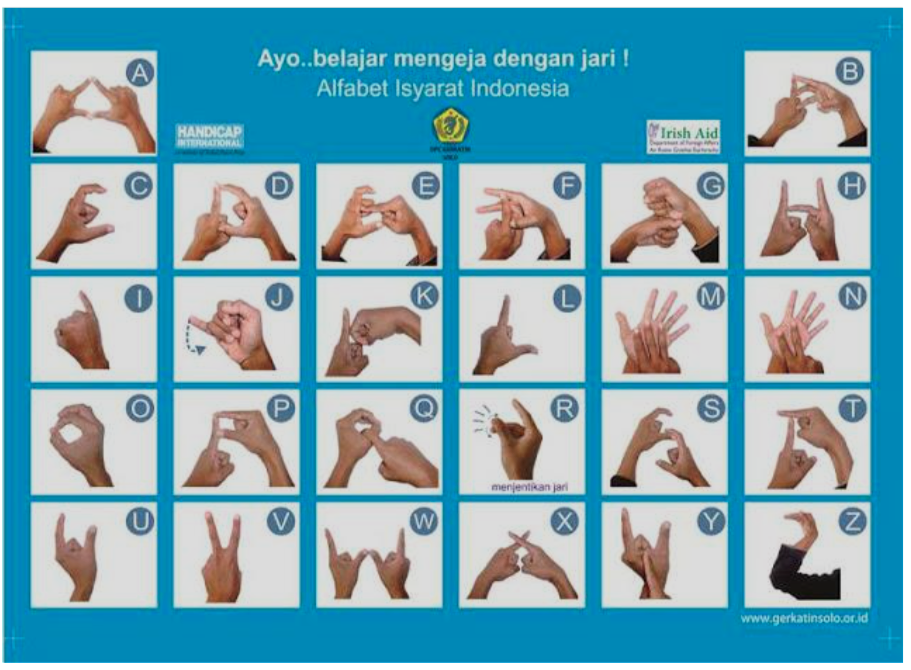
\includegraphics[width=\textwidth]{BAB-2/figures/alfabetbisindo.png}	
%	    \caption{Alfabet Bisindo (Almuharram, 2013).}
%	    \label{gambar:alfabet bisindo}
%\end{figure}
%\end{center}
%Gambar \ref{gambar:alfabet bisindo} menyunjukkan sudut pandang umum yang digunakan dalam berkomunikasi menggunakan bahasa isyarat, yaitu tampak depan \citep{xiong2004_dscForSensorNetworks}. Sehingga, data gambar yang digunakan di penelitian ini juga memuat gestur Bisindo dari tampak depan, dengan persamaan~(\ref{func:loss}), dengan hasil penelitian di Bab~\ref{BAB4:hasil}.